% Options for packages loaded elsewhere
\PassOptionsToPackage{unicode}{hyperref}
\PassOptionsToPackage{hyphens}{url}
\PassOptionsToPackage{dvipsnames,svgnames,x11names}{xcolor}
%
\documentclass[
  letterpaper,
  DIV=11,
  numbers=noendperiod]{scrartcl}

\usepackage{amsmath,amssymb}
\usepackage{iftex}
\ifPDFTeX
  \usepackage[T1]{fontenc}
  \usepackage[utf8]{inputenc}
  \usepackage{textcomp} % provide euro and other symbols
\else % if luatex or xetex
  \usepackage{unicode-math}
  \defaultfontfeatures{Scale=MatchLowercase}
  \defaultfontfeatures[\rmfamily]{Ligatures=TeX,Scale=1}
\fi
\usepackage{lmodern}
\ifPDFTeX\else  
    % xetex/luatex font selection
\fi
% Use upquote if available, for straight quotes in verbatim environments
\IfFileExists{upquote.sty}{\usepackage{upquote}}{}
\IfFileExists{microtype.sty}{% use microtype if available
  \usepackage[]{microtype}
  \UseMicrotypeSet[protrusion]{basicmath} % disable protrusion for tt fonts
}{}
\makeatletter
\@ifundefined{KOMAClassName}{% if non-KOMA class
  \IfFileExists{parskip.sty}{%
    \usepackage{parskip}
  }{% else
    \setlength{\parindent}{0pt}
    \setlength{\parskip}{6pt plus 2pt minus 1pt}}
}{% if KOMA class
  \KOMAoptions{parskip=half}}
\makeatother
\usepackage{xcolor}
\setlength{\emergencystretch}{3em} % prevent overfull lines
\setcounter{secnumdepth}{-\maxdimen} % remove section numbering
% Make \paragraph and \subparagraph free-standing
\makeatletter
\ifx\paragraph\undefined\else
  \let\oldparagraph\paragraph
  \renewcommand{\paragraph}{
    \@ifstar
      \xxxParagraphStar
      \xxxParagraphNoStar
  }
  \newcommand{\xxxParagraphStar}[1]{\oldparagraph*{#1}\mbox{}}
  \newcommand{\xxxParagraphNoStar}[1]{\oldparagraph{#1}\mbox{}}
\fi
\ifx\subparagraph\undefined\else
  \let\oldsubparagraph\subparagraph
  \renewcommand{\subparagraph}{
    \@ifstar
      \xxxSubParagraphStar
      \xxxSubParagraphNoStar
  }
  \newcommand{\xxxSubParagraphStar}[1]{\oldsubparagraph*{#1}\mbox{}}
  \newcommand{\xxxSubParagraphNoStar}[1]{\oldsubparagraph{#1}\mbox{}}
\fi
\makeatother

\usepackage{color}
\usepackage{fancyvrb}
\newcommand{\VerbBar}{|}
\newcommand{\VERB}{\Verb[commandchars=\\\{\}]}
\DefineVerbatimEnvironment{Highlighting}{Verbatim}{commandchars=\\\{\}}
% Add ',fontsize=\small' for more characters per line
\usepackage{framed}
\definecolor{shadecolor}{RGB}{241,243,245}
\newenvironment{Shaded}{\begin{snugshade}}{\end{snugshade}}
\newcommand{\AlertTok}[1]{\textcolor[rgb]{0.68,0.00,0.00}{#1}}
\newcommand{\AnnotationTok}[1]{\textcolor[rgb]{0.37,0.37,0.37}{#1}}
\newcommand{\AttributeTok}[1]{\textcolor[rgb]{0.40,0.45,0.13}{#1}}
\newcommand{\BaseNTok}[1]{\textcolor[rgb]{0.68,0.00,0.00}{#1}}
\newcommand{\BuiltInTok}[1]{\textcolor[rgb]{0.00,0.23,0.31}{#1}}
\newcommand{\CharTok}[1]{\textcolor[rgb]{0.13,0.47,0.30}{#1}}
\newcommand{\CommentTok}[1]{\textcolor[rgb]{0.37,0.37,0.37}{#1}}
\newcommand{\CommentVarTok}[1]{\textcolor[rgb]{0.37,0.37,0.37}{\textit{#1}}}
\newcommand{\ConstantTok}[1]{\textcolor[rgb]{0.56,0.35,0.01}{#1}}
\newcommand{\ControlFlowTok}[1]{\textcolor[rgb]{0.00,0.23,0.31}{\textbf{#1}}}
\newcommand{\DataTypeTok}[1]{\textcolor[rgb]{0.68,0.00,0.00}{#1}}
\newcommand{\DecValTok}[1]{\textcolor[rgb]{0.68,0.00,0.00}{#1}}
\newcommand{\DocumentationTok}[1]{\textcolor[rgb]{0.37,0.37,0.37}{\textit{#1}}}
\newcommand{\ErrorTok}[1]{\textcolor[rgb]{0.68,0.00,0.00}{#1}}
\newcommand{\ExtensionTok}[1]{\textcolor[rgb]{0.00,0.23,0.31}{#1}}
\newcommand{\FloatTok}[1]{\textcolor[rgb]{0.68,0.00,0.00}{#1}}
\newcommand{\FunctionTok}[1]{\textcolor[rgb]{0.28,0.35,0.67}{#1}}
\newcommand{\ImportTok}[1]{\textcolor[rgb]{0.00,0.46,0.62}{#1}}
\newcommand{\InformationTok}[1]{\textcolor[rgb]{0.37,0.37,0.37}{#1}}
\newcommand{\KeywordTok}[1]{\textcolor[rgb]{0.00,0.23,0.31}{\textbf{#1}}}
\newcommand{\NormalTok}[1]{\textcolor[rgb]{0.00,0.23,0.31}{#1}}
\newcommand{\OperatorTok}[1]{\textcolor[rgb]{0.37,0.37,0.37}{#1}}
\newcommand{\OtherTok}[1]{\textcolor[rgb]{0.00,0.23,0.31}{#1}}
\newcommand{\PreprocessorTok}[1]{\textcolor[rgb]{0.68,0.00,0.00}{#1}}
\newcommand{\RegionMarkerTok}[1]{\textcolor[rgb]{0.00,0.23,0.31}{#1}}
\newcommand{\SpecialCharTok}[1]{\textcolor[rgb]{0.37,0.37,0.37}{#1}}
\newcommand{\SpecialStringTok}[1]{\textcolor[rgb]{0.13,0.47,0.30}{#1}}
\newcommand{\StringTok}[1]{\textcolor[rgb]{0.13,0.47,0.30}{#1}}
\newcommand{\VariableTok}[1]{\textcolor[rgb]{0.07,0.07,0.07}{#1}}
\newcommand{\VerbatimStringTok}[1]{\textcolor[rgb]{0.13,0.47,0.30}{#1}}
\newcommand{\WarningTok}[1]{\textcolor[rgb]{0.37,0.37,0.37}{\textit{#1}}}

\providecommand{\tightlist}{%
  \setlength{\itemsep}{0pt}\setlength{\parskip}{0pt}}\usepackage{longtable,booktabs,array}
\usepackage{calc} % for calculating minipage widths
% Correct order of tables after \paragraph or \subparagraph
\usepackage{etoolbox}
\makeatletter
\patchcmd\longtable{\par}{\if@noskipsec\mbox{}\fi\par}{}{}
\makeatother
% Allow footnotes in longtable head/foot
\IfFileExists{footnotehyper.sty}{\usepackage{footnotehyper}}{\usepackage{footnote}}
\makesavenoteenv{longtable}
\usepackage{graphicx}
\makeatletter
\def\maxwidth{\ifdim\Gin@nat@width>\linewidth\linewidth\else\Gin@nat@width\fi}
\def\maxheight{\ifdim\Gin@nat@height>\textheight\textheight\else\Gin@nat@height\fi}
\makeatother
% Scale images if necessary, so that they will not overflow the page
% margins by default, and it is still possible to overwrite the defaults
% using explicit options in \includegraphics[width, height, ...]{}
\setkeys{Gin}{width=\maxwidth,height=\maxheight,keepaspectratio}
% Set default figure placement to htbp
\makeatletter
\def\fps@figure{htbp}
\makeatother

\usepackage{fvextra}
\DefineVerbatimEnvironment{Highlighting}{Verbatim}{breaklines,commandchars=\\\{\}}
\KOMAoption{captions}{tableheading}
\makeatletter
\@ifpackageloaded{caption}{}{\usepackage{caption}}
\AtBeginDocument{%
\ifdefined\contentsname
  \renewcommand*\contentsname{Table of contents}
\else
  \newcommand\contentsname{Table of contents}
\fi
\ifdefined\listfigurename
  \renewcommand*\listfigurename{List of Figures}
\else
  \newcommand\listfigurename{List of Figures}
\fi
\ifdefined\listtablename
  \renewcommand*\listtablename{List of Tables}
\else
  \newcommand\listtablename{List of Tables}
\fi
\ifdefined\figurename
  \renewcommand*\figurename{Figure}
\else
  \newcommand\figurename{Figure}
\fi
\ifdefined\tablename
  \renewcommand*\tablename{Table}
\else
  \newcommand\tablename{Table}
\fi
}
\@ifpackageloaded{float}{}{\usepackage{float}}
\floatstyle{ruled}
\@ifundefined{c@chapter}{\newfloat{codelisting}{h}{lop}}{\newfloat{codelisting}{h}{lop}[chapter]}
\floatname{codelisting}{Listing}
\newcommand*\listoflistings{\listof{codelisting}{List of Listings}}
\makeatother
\makeatletter
\makeatother
\makeatletter
\@ifpackageloaded{caption}{}{\usepackage{caption}}
\@ifpackageloaded{subcaption}{}{\usepackage{subcaption}}
\makeatother

\ifLuaTeX
  \usepackage{selnolig}  % disable illegal ligatures
\fi
\usepackage{bookmark}

\IfFileExists{xurl.sty}{\usepackage{xurl}}{} % add URL line breaks if available
\urlstyle{same} % disable monospaced font for URLs
\hypersetup{
  pdftitle={Problem Set 6 - Waze Shiny Dashboard},
  pdfauthor={Peter Ganong, Maggie Shi, and Andre Oviedo},
  colorlinks=true,
  linkcolor={blue},
  filecolor={Maroon},
  citecolor={Blue},
  urlcolor={Blue},
  pdfcreator={LaTeX via pandoc}}


\title{Problem Set 6 - Waze Shiny Dashboard}
\author{Peter Ganong, Maggie Shi, and Andre Oviedo}
\date{2024-11-23}

\begin{document}
\maketitle

\RecustomVerbatimEnvironment{verbatim}{Verbatim}{
  showspaces = false,
  showtabs = false,
  breaksymbolleft={},
  breaklines
}


\begin{enumerate}
\def\labelenumi{\arabic{enumi}.}
\tightlist
\item
  \textbf{ps6:} Due Sat 23rd at 5:00PM Central. Worth 100 points (80
  points from questions, 10 points for correct submission and 10 points
  for code style) + 10 extra credit.
\end{enumerate}

We use (\texttt{*}) to indicate a problem that we think might be time
consuming.

\section*{Steps to submit (10 points on
PS6)}\label{steps-to-submit-10-points-on-ps6}
\addcontentsline{toc}{section}{Steps to submit (10 points on PS6)}

\begin{enumerate}
\def\labelenumi{\arabic{enumi}.}
\item
  ``This submission is my work alone and complies with the 30538
  integrity policy.'' Add your initials to indicate your agreement:
  \textbf{KC}
\item
  ``I have uploaded the names of anyone I worked with on the problem set
  \textbf{\href{https://docs.google.com/forms/d/185usrCREQaUbvAXpWhChkjghdGgmAZXA3lPWpXLLsts/edit}{here}}''
  \textbf{KC} (2 point)
\item
  Late coins used this pset: \textbf{0} Late coins left after
  submission: \textbf{3}
\item
  Before starting the problem set, make sure to read and agree to the
  terms of data usage for the Waze data
  \href{https://canvas.uchicago.edu/courses/59054/quizzes/130617}{here}.
\item
  Knit your \texttt{ps6.qmd} as a pdf document and name it
  \texttt{ps6.pdf}.
\item
  Push your \texttt{ps6.qmd}, \texttt{ps6.pdf},
  \texttt{requirements.txt}, and all created folders (we will create
  three Shiny apps so you will have at least three additional folders)
  to your Github repo (5 points). It is fine to use Github Desktop.
\item
  Submit \texttt{ps6.pdf} and also link your Github repo via Gradescope
  (5 points)
\item
  Tag your submission in Gradescope. For the Code Style part (10 points)
  please tag the whole correspondingsection for the code style rubric.
\end{enumerate}

\emph{Notes: see the
\href{https://quarto.org/docs/authoring/figures.html}{Quarto
documentation (link)} for directions on inserting images into your
knitted document.}

\emph{IMPORTANT: For the App portion of the PS, in case you can not
arrive to the expected functional dashboard we will need to take a look
at your \texttt{app.py} file. You can use the following code chunk
template to ``import'' and print the content of that file. Please, don't
forget to also tag the corresponding code chunk as part of your
submission!}

\begin{Shaded}
\begin{Highlighting}[]
\KeywordTok{def}\NormalTok{ print\_file\_contents(file\_path):}
    \CommentTok{"""Print contents of a file."""}
    \ControlFlowTok{try}\NormalTok{:}
        \ControlFlowTok{with} \BuiltInTok{open}\NormalTok{(file\_path, }\StringTok{\textquotesingle{}r\textquotesingle{}}\NormalTok{) }\ImportTok{as}\NormalTok{ f:}
\NormalTok{            content }\OperatorTok{=}\NormalTok{ f.read()}
            \BuiltInTok{print}\NormalTok{(}\StringTok{"\textasciigrave{}\textasciigrave{}\textasciigrave{}python"}\NormalTok{)}
            \BuiltInTok{print}\NormalTok{(content)}
            \BuiltInTok{print}\NormalTok{(}\StringTok{"\textasciigrave{}\textasciigrave{}\textasciigrave{}"}\NormalTok{)}
    \ControlFlowTok{except} \PreprocessorTok{FileNotFoundError}\NormalTok{:}
        \BuiltInTok{print}\NormalTok{(}\StringTok{"\textasciigrave{}\textasciigrave{}\textasciigrave{}python"}\NormalTok{)}
        \BuiltInTok{print}\NormalTok{(}\SpecialStringTok{f"Error: File \textquotesingle{}}\SpecialCharTok{\{}\NormalTok{file\_path}\SpecialCharTok{\}}\SpecialStringTok{\textquotesingle{} not found"}\NormalTok{)}
        \BuiltInTok{print}\NormalTok{(}\StringTok{"\textasciigrave{}\textasciigrave{}\textasciigrave{}"}\NormalTok{)}
    \ControlFlowTok{except} \PreprocessorTok{Exception} \ImportTok{as}\NormalTok{ e:}
        \BuiltInTok{print}\NormalTok{(}\StringTok{"\textasciigrave{}\textasciigrave{}\textasciigrave{}python"}\NormalTok{) }
        \BuiltInTok{print}\NormalTok{(}\SpecialStringTok{f"Error reading file: }\SpecialCharTok{\{}\NormalTok{e}\SpecialCharTok{\}}\SpecialStringTok{"}\NormalTok{)}
        \BuiltInTok{print}\NormalTok{(}\StringTok{"\textasciigrave{}\textasciigrave{}\textasciigrave{}"}\NormalTok{)}

\NormalTok{print\_file\_contents(}\StringTok{"./top\_alerts\_map\_byhour/app.py"}\NormalTok{) }\CommentTok{\# Change accordingly}
\end{Highlighting}
\end{Shaded}

\section*{Background}\label{background}
\addcontentsline{toc}{section}{Background}

\subsection*{Data Download and Exploration (20
points)}\label{data-download-and-exploration-20-points}
\addcontentsline{toc}{subsection}{Data Download and Exploration (20
points)}

\begin{enumerate}
\def\labelenumi{\arabic{enumi}.}
\tightlist
\item
\end{enumerate}

\begin{Shaded}
\begin{Highlighting}[]
\CommentTok{\# Read the sample data}
\NormalTok{df\_sample }\OperatorTok{=}\NormalTok{ pd.read\_csv(}\StringTok{"/Users/kohanchen/Documents/Fall 2024/student30538/problem\_sets/ps6/waze\_data/waze\_data\_sample.csv"}\NormalTok{)}

\CommentTok{\# Get column names and types, excluding specified columns}
\NormalTok{cols\_to\_skip }\OperatorTok{=}\NormalTok{ [}\StringTok{\textquotesingle{}ts\textquotesingle{}}\NormalTok{, }\StringTok{\textquotesingle{}geo\textquotesingle{}}\NormalTok{, }\StringTok{\textquotesingle{}geoWKT\textquotesingle{}}\NormalTok{]}
\NormalTok{col\_info }\OperatorTok{=}\NormalTok{ [(col, }\BuiltInTok{str}\NormalTok{(df\_sample[col].dtype)) }\ControlFlowTok{for}\NormalTok{ col }\KeywordTok{in}\NormalTok{ df\_sample.columns }\ControlFlowTok{if}\NormalTok{ col }\KeywordTok{not} \KeywordTok{in}\NormalTok{ cols\_to\_skip]}

\BuiltInTok{print}\NormalTok{(}\StringTok{"Column names and their Altair data types:"}\NormalTok{)}
\ControlFlowTok{for}\NormalTok{ col, dtype }\KeywordTok{in}\NormalTok{ col\_info:}
    \CommentTok{\# Map pandas dtypes to Altair types}
    \ControlFlowTok{if}\NormalTok{ dtype.startswith(}\StringTok{\textquotesingle{}int\textquotesingle{}}\NormalTok{) }\KeywordTok{or}\NormalTok{ dtype.startswith(}\StringTok{\textquotesingle{}float\textquotesingle{}}\NormalTok{):}
\NormalTok{        alt\_type }\OperatorTok{=} \StringTok{"Quantitative"}
    \ControlFlowTok{elif}\NormalTok{ dtype }\OperatorTok{==} \StringTok{\textquotesingle{}object\textquotesingle{}} \KeywordTok{or}\NormalTok{ dtype }\OperatorTok{==} \StringTok{\textquotesingle{}category\textquotesingle{}}\NormalTok{:}
\NormalTok{        alt\_type }\OperatorTok{=} \StringTok{"Nominal"}
    \ControlFlowTok{elif}\NormalTok{ dtype.startswith(}\StringTok{\textquotesingle{}datetime\textquotesingle{}}\NormalTok{):}
\NormalTok{        alt\_type }\OperatorTok{=} \StringTok{"Temporal"}
    \ControlFlowTok{else}\NormalTok{:}
\NormalTok{        alt\_type }\OperatorTok{=} \StringTok{"Unknown"}
        
    \BuiltInTok{print}\NormalTok{(}\SpecialStringTok{f"}\SpecialCharTok{\{}\NormalTok{col}\SpecialCharTok{\}}\SpecialStringTok{: }\SpecialCharTok{\{}\NormalTok{alt\_type}\SpecialCharTok{\}}\SpecialStringTok{"}\NormalTok{)}
\end{Highlighting}
\end{Shaded}

\begin{verbatim}
Column names and their Altair data types:
Unnamed: 0: Quantitative
city: Nominal
confidence: Quantitative
nThumbsUp: Quantitative
street: Nominal
uuid: Nominal
country: Nominal
type: Nominal
subtype: Nominal
roadType: Quantitative
reliability: Quantitative
magvar: Quantitative
reportRating: Quantitative
\end{verbatim}

\begin{enumerate}
\def\labelenumi{\arabic{enumi}.}
\setcounter{enumi}{1}
\tightlist
\item
\end{enumerate}

\begin{Shaded}
\begin{Highlighting}[]
\NormalTok{df\_full }\OperatorTok{=}\NormalTok{ pd.read\_csv(}\StringTok{"/Users/kohanchen/Documents/Fall 2024/student30538/problem\_sets/ps6/waze\_data/waze\_data.csv"}\NormalTok{)}

\NormalTok{null\_counts }\OperatorTok{=}\NormalTok{ pd.DataFrame(\{}
    \StringTok{\textquotesingle{}Variable\textquotesingle{}}\NormalTok{: df\_full.columns,}
    \StringTok{\textquotesingle{}Missing\textquotesingle{}}\NormalTok{: df\_full.isnull().}\BuiltInTok{sum}\NormalTok{(),}
    \StringTok{\textquotesingle{}Not Missing\textquotesingle{}}\NormalTok{: df\_full.notnull().}\BuiltInTok{sum}\NormalTok{()}
\NormalTok{\}).melt(id\_vars}\OperatorTok{=}\NormalTok{[}\StringTok{\textquotesingle{}Variable\textquotesingle{}}\NormalTok{], var\_name}\OperatorTok{=}\StringTok{\textquotesingle{}Status\textquotesingle{}}\NormalTok{, value\_name}\OperatorTok{=}\StringTok{\textquotesingle{}Count\textquotesingle{}}\NormalTok{)}

\CommentTok{\# Create stacked bar chart}
\NormalTok{chart }\OperatorTok{=}\NormalTok{ alt.Chart(null\_counts).mark\_bar().encode(}
\NormalTok{    x}\OperatorTok{=}\NormalTok{alt.X(}\StringTok{\textquotesingle{}Variable:N\textquotesingle{}}\NormalTok{, title}\OperatorTok{=}\StringTok{\textquotesingle{}Variables\textquotesingle{}}\NormalTok{),}
\NormalTok{    y}\OperatorTok{=}\NormalTok{alt.Y(}\StringTok{\textquotesingle{}Count:Q\textquotesingle{}}\NormalTok{, }
\NormalTok{            title}\OperatorTok{=}\StringTok{\textquotesingle{}Number of Observations\textquotesingle{}}\NormalTok{,}
\NormalTok{            stack}\OperatorTok{=}\StringTok{\textquotesingle{}normalize\textquotesingle{}}\NormalTok{),  }\CommentTok{\# stack parameter goes inside Y encoding}
\NormalTok{    color}\OperatorTok{=}\NormalTok{alt.Color(}\StringTok{\textquotesingle{}Status:N\textquotesingle{}}\NormalTok{, scale}\OperatorTok{=}\NormalTok{alt.Scale(scheme}\OperatorTok{=}\StringTok{\textquotesingle{}set2\textquotesingle{}}\NormalTok{)),}
\NormalTok{    tooltip}\OperatorTok{=}\NormalTok{[}
\NormalTok{        alt.Tooltip(}\StringTok{\textquotesingle{}Variable:N\textquotesingle{}}\NormalTok{),}
\NormalTok{        alt.Tooltip(}\StringTok{\textquotesingle{}Status:N\textquotesingle{}}\NormalTok{),}
\NormalTok{        alt.Tooltip(}\StringTok{\textquotesingle{}Count:Q\textquotesingle{}}\NormalTok{, }\BuiltInTok{format}\OperatorTok{=}\StringTok{\textquotesingle{},\textquotesingle{}}\NormalTok{),}
\NormalTok{        alt.Tooltip(}\StringTok{\textquotesingle{}Count:Q\textquotesingle{}}\NormalTok{, aggregate}\OperatorTok{=}\StringTok{\textquotesingle{}sum\textquotesingle{}}\NormalTok{, title}\OperatorTok{=}\StringTok{\textquotesingle{}Total Rows\textquotesingle{}}\NormalTok{, }\BuiltInTok{format}\OperatorTok{=}\StringTok{\textquotesingle{},\textquotesingle{}}\NormalTok{)}
\NormalTok{    ]}
\NormalTok{).properties(}
\NormalTok{    title}\OperatorTok{=}\StringTok{\textquotesingle{}Distribution of Missing vs Non{-}Missing Values by Variable\textquotesingle{}}
\NormalTok{)}
\end{Highlighting}
\end{Shaded}

nThumbsUp, Street, and subtypes have missing values. And nThumbsUp has
the highest share of missing values. 3.

\begin{Shaded}
\begin{Highlighting}[]
\BuiltInTok{print}\NormalTok{(}\StringTok{"Unique values in \textquotesingle{}type\textquotesingle{}:"}\NormalTok{)}
\BuiltInTok{print}\NormalTok{(df\_full[}\StringTok{\textquotesingle{}type\textquotesingle{}}\NormalTok{].unique())}

\BuiltInTok{print}\NormalTok{(}\StringTok{"All unique values in \textquotesingle{}subtype\textquotesingle{}:"}\NormalTok{)}
\CommentTok{\# Filter out NaN values before sorting}
\NormalTok{unique\_subtypes }\OperatorTok{=}\NormalTok{ df\_full[}\StringTok{\textquotesingle{}subtype\textquotesingle{}}\NormalTok{].dropna().unique()}
\BuiltInTok{print}\NormalTok{(}\BuiltInTok{sorted}\NormalTok{(unique\_subtypes))}

\CommentTok{\# Create crosswalk DataFrames}
\NormalTok{type\_crosswalk }\OperatorTok{=}\NormalTok{ pd.DataFrame(\{}
    \StringTok{\textquotesingle{}original\textquotesingle{}}\NormalTok{: [}\StringTok{\textquotesingle{}ROAD\_CLOSED\textquotesingle{}}\NormalTok{, }\StringTok{\textquotesingle{}JAM\textquotesingle{}}\NormalTok{, }\StringTok{\textquotesingle{}ACCIDENT\textquotesingle{}}\NormalTok{, }\StringTok{\textquotesingle{}HAZARD\textquotesingle{}}\NormalTok{],}
    \StringTok{\textquotesingle{}clean\_name\textquotesingle{}}\NormalTok{: [}\StringTok{\textquotesingle{}Road Closure\textquotesingle{}}\NormalTok{, }\StringTok{\textquotesingle{}Traffic Jam\textquotesingle{}}\NormalTok{, }\StringTok{\textquotesingle{}Accident\textquotesingle{}}\NormalTok{, }\StringTok{\textquotesingle{}Hazard\textquotesingle{}}\NormalTok{] \})}

\NormalTok{subtype\_crosswalk }\OperatorTok{=}\NormalTok{ pd.DataFrame(\{}
    \StringTok{\textquotesingle{}original\textquotesingle{}}\NormalTok{: [}
        \CommentTok{\# Accidents}
        \StringTok{\textquotesingle{}ACCIDENT\_MAJOR\textquotesingle{}}\NormalTok{,}
        \StringTok{\textquotesingle{}ACCIDENT\_MINOR\textquotesingle{}}\NormalTok{,}
        
        \CommentTok{\# Jams}
        \StringTok{\textquotesingle{}JAM\_HEAVY\_TRAFFIC\textquotesingle{}}\NormalTok{,}
        \StringTok{\textquotesingle{}JAM\_LIGHT\_TRAFFIC\textquotesingle{}}\NormalTok{,}
        \StringTok{\textquotesingle{}JAM\_MODERATE\_TRAFFIC\textquotesingle{}}\NormalTok{,}
        \StringTok{\textquotesingle{}JAM\_STAND\_STILL\_TRAFFIC\textquotesingle{}}\NormalTok{,}
        
        \CommentTok{\# Road Closures}
        \StringTok{\textquotesingle{}ROAD\_CLOSED\_CONSTRUCTION\textquotesingle{}}\NormalTok{,}
        \StringTok{\textquotesingle{}ROAD\_CLOSED\_EVENT\textquotesingle{}}\NormalTok{,}
        \StringTok{\textquotesingle{}ROAD\_CLOSED\_HAZARD\textquotesingle{}}\NormalTok{,}
        
        \CommentTok{\# Road Hazards}
        \StringTok{\textquotesingle{}HAZARD\_ON\_ROAD\textquotesingle{}}\NormalTok{,}
        \StringTok{\textquotesingle{}HAZARD\_ON\_ROAD\_CAR\_STOPPED\textquotesingle{}}\NormalTok{,}
        \StringTok{\textquotesingle{}HAZARD\_ON\_ROAD\_CONSTRUCTION\textquotesingle{}}\NormalTok{,}
        \StringTok{\textquotesingle{}HAZARD\_ON\_ROAD\_EMERGENCY\_VEHICLE\textquotesingle{}}\NormalTok{,}
        \StringTok{\textquotesingle{}HAZARD\_ON\_ROAD\_ICE\textquotesingle{}}\NormalTok{,}
        \StringTok{\textquotesingle{}HAZARD\_ON\_ROAD\_LANE\_CLOSED\textquotesingle{}}\NormalTok{,}
        \StringTok{\textquotesingle{}HAZARD\_ON\_ROAD\_OBJECT\textquotesingle{}}\NormalTok{,}
        \StringTok{\textquotesingle{}HAZARD\_ON\_ROAD\_POT\_HOLE\textquotesingle{}}\NormalTok{,}
        \StringTok{\textquotesingle{}HAZARD\_ON\_ROAD\_ROAD\_KILL\textquotesingle{}}\NormalTok{,}
        \StringTok{\textquotesingle{}HAZARD\_ON\_ROAD\_TRAFFIC\_LIGHT\_FAULT\textquotesingle{}}\NormalTok{,}
        
        \CommentTok{\# Shoulder Hazards}
        \StringTok{\textquotesingle{}HAZARD\_ON\_SHOULDER\textquotesingle{}}\NormalTok{,}
        \StringTok{\textquotesingle{}HAZARD\_ON\_SHOULDER\_ANIMALS\textquotesingle{}}\NormalTok{,}
        \StringTok{\textquotesingle{}HAZARD\_ON\_SHOULDER\_CAR\_STOPPED\textquotesingle{}}\NormalTok{,}
        \StringTok{\textquotesingle{}HAZARD\_ON\_SHOULDER\_MISSING\_SIGN\textquotesingle{}}\NormalTok{,}

                \CommentTok{\# Weather Hazards}
        \StringTok{\textquotesingle{}HAZARD\_WEATHER\textquotesingle{}}\NormalTok{,}
        \StringTok{\textquotesingle{}HAZARD\_WEATHER\_FLOOD\textquotesingle{}}\NormalTok{,}
        \StringTok{\textquotesingle{}HAZARD\_WEATHER\_FOG\textquotesingle{}}\NormalTok{,}
        \StringTok{\textquotesingle{}HAZARD\_WEATHER\_HAIL\textquotesingle{}}\NormalTok{,}
        \StringTok{\textquotesingle{}HAZARD\_WEATHER\_HEAVY\_SNOW\textquotesingle{}}
\NormalTok{    ],}
    \StringTok{\textquotesingle{}clean\_name\textquotesingle{}}\NormalTok{: [}
        \CommentTok{\# Accidents}
        \StringTok{\textquotesingle{}Major Accident\textquotesingle{}}\NormalTok{,}
        \StringTok{\textquotesingle{}Minor Accident\textquotesingle{}}\NormalTok{,}
        
        \CommentTok{\# Jams}
        \StringTok{\textquotesingle{}Heavy Traffic\textquotesingle{}}\NormalTok{,}
        \StringTok{\textquotesingle{}Light Traffic\textquotesingle{}}\NormalTok{,}
        \StringTok{\textquotesingle{}Moderate Traffic\textquotesingle{}}\NormalTok{,}
        \StringTok{\textquotesingle{}Standstill Traffic\textquotesingle{}}\NormalTok{,}
        
        \CommentTok{\# Road Closures}
        \StringTok{\textquotesingle{}Construction Closure\textquotesingle{}}\NormalTok{,}
        \StringTok{\textquotesingle{}Event Closure\textquotesingle{}}\NormalTok{,}
        \StringTok{\textquotesingle{}Hazard Closure\textquotesingle{}}\NormalTok{,}
        
        \CommentTok{\# Road Hazards}
        \StringTok{\textquotesingle{}Road Hazard\textquotesingle{}}\NormalTok{,}
        \StringTok{\textquotesingle{}Stopped Vehicle on Road\textquotesingle{}}\NormalTok{,}
        \StringTok{\textquotesingle{}Construction on Road\textquotesingle{}}\NormalTok{,}
        \StringTok{\textquotesingle{}Emergency Vehicle\textquotesingle{}}\NormalTok{,}
        \StringTok{\textquotesingle{}Ice on Road\textquotesingle{}}\NormalTok{,}
        \StringTok{\textquotesingle{}Lane Closure\textquotesingle{}}\NormalTok{,}
        \StringTok{\textquotesingle{}Object on Road\textquotesingle{}}\NormalTok{,}
        \StringTok{\textquotesingle{}Pothole\textquotesingle{}}\NormalTok{,}
        \StringTok{\textquotesingle{}Road Kill\textquotesingle{}}\NormalTok{,}
        \StringTok{\textquotesingle{}Traffic Light Issue\textquotesingle{}}\NormalTok{,}
        
        \CommentTok{\# Shoulder Hazards}
        \StringTok{\textquotesingle{}Shoulder Hazard\textquotesingle{}}\NormalTok{,}
        \StringTok{\textquotesingle{}Animals on Shoulder\textquotesingle{}}\NormalTok{,}
        \StringTok{\textquotesingle{}Stopped Vehicle on Shoulder\textquotesingle{}}\NormalTok{,}
        \StringTok{\textquotesingle{}Missing Sign\textquotesingle{}}\NormalTok{,}
        
        \CommentTok{\# Weather Hazards}
        \StringTok{\textquotesingle{}Weather Hazard\textquotesingle{}}\NormalTok{,}
        \StringTok{\textquotesingle{}Flooding\textquotesingle{}}\NormalTok{,}
        \StringTok{\textquotesingle{}Fog\textquotesingle{}}\NormalTok{,}
        \StringTok{\textquotesingle{}Hail\textquotesingle{}}\NormalTok{,}
        \StringTok{\textquotesingle{}Heavy Snow\textquotesingle{}}
\NormalTok{    ]}
\NormalTok{\})}
\CommentTok{\# Create mapping dictionaries}
\NormalTok{type\_mapping }\OperatorTok{=} \BuiltInTok{dict}\NormalTok{(}\BuiltInTok{zip}\NormalTok{(type\_crosswalk[}\StringTok{\textquotesingle{}original\textquotesingle{}}\NormalTok{], type\_crosswalk[}\StringTok{\textquotesingle{}clean\_name\textquotesingle{}}\NormalTok{]))}
\NormalTok{subtype\_mapping }\OperatorTok{=} \BuiltInTok{dict}\NormalTok{(}\BuiltInTok{zip}\NormalTok{(subtype\_crosswalk[}\StringTok{\textquotesingle{}original\textquotesingle{}}\NormalTok{], subtype\_crosswalk[}\StringTok{\textquotesingle{}clean\_name\textquotesingle{}}\NormalTok{]))}

\CommentTok{\# Apply mappings while preserving NaN values}
\NormalTok{df\_full[}\StringTok{\textquotesingle{}type\_clean\textquotesingle{}}\NormalTok{] }\OperatorTok{=}\NormalTok{ df\_full[}\StringTok{\textquotesingle{}type\textquotesingle{}}\NormalTok{].}\BuiltInTok{map}\NormalTok{(type\_mapping)}
\NormalTok{df\_full[}\StringTok{\textquotesingle{}subtype\_clean\textquotesingle{}}\NormalTok{] }\OperatorTok{=}\NormalTok{ df\_full[}\StringTok{\textquotesingle{}subtype\textquotesingle{}}\NormalTok{].}\BuiltInTok{map}\NormalTok{(subtype\_mapping)}

\CommentTok{\# Verify the results}
\BuiltInTok{print}\NormalTok{(}\StringTok{"Sample of cleaned data (including some rows with non{-}null subtypes):"}\NormalTok{)}
\BuiltInTok{print}\NormalTok{(df\_full[df\_full[}\StringTok{\textquotesingle{}subtype\textquotesingle{}}\NormalTok{].notna()][[}\StringTok{\textquotesingle{}type\textquotesingle{}}\NormalTok{, }\StringTok{\textquotesingle{}type\_clean\textquotesingle{}}\NormalTok{, }\StringTok{\textquotesingle{}subtype\textquotesingle{}}\NormalTok{, }\StringTok{\textquotesingle{}subtype\_clean\textquotesingle{}}\NormalTok{]].head())}
\end{Highlighting}
\end{Shaded}

\begin{verbatim}
Unique values in 'type':
['JAM' 'ACCIDENT' 'ROAD_CLOSED' 'HAZARD']
All unique values in 'subtype':
['ACCIDENT_MAJOR', 'ACCIDENT_MINOR', 'HAZARD_ON_ROAD', 'HAZARD_ON_ROAD_CAR_STOPPED', 'HAZARD_ON_ROAD_CONSTRUCTION', 'HAZARD_ON_ROAD_EMERGENCY_VEHICLE', 'HAZARD_ON_ROAD_ICE', 'HAZARD_ON_ROAD_LANE_CLOSED', 'HAZARD_ON_ROAD_OBJECT', 'HAZARD_ON_ROAD_POT_HOLE', 'HAZARD_ON_ROAD_ROAD_KILL', 'HAZARD_ON_ROAD_TRAFFIC_LIGHT_FAULT', 'HAZARD_ON_SHOULDER', 'HAZARD_ON_SHOULDER_ANIMALS', 'HAZARD_ON_SHOULDER_CAR_STOPPED', 'HAZARD_ON_SHOULDER_MISSING_SIGN', 'HAZARD_WEATHER', 'HAZARD_WEATHER_FLOOD', 'HAZARD_WEATHER_FOG', 'HAZARD_WEATHER_HAIL', 'HAZARD_WEATHER_HEAVY_SNOW', 'JAM_HEAVY_TRAFFIC', 'JAM_LIGHT_TRAFFIC', 'JAM_MODERATE_TRAFFIC', 'JAM_STAND_STILL_TRAFFIC', 'ROAD_CLOSED_CONSTRUCTION', 'ROAD_CLOSED_EVENT', 'ROAD_CLOSED_HAZARD']
Sample of cleaned data (including some rows with non-null subtypes):
         type type_clean         subtype   subtype_clean
122  ACCIDENT   Accident  ACCIDENT_MAJOR  Major Accident
123  ACCIDENT   Accident  ACCIDENT_MAJOR  Major Accident
124  ACCIDENT   Accident  ACCIDENT_MAJOR  Major Accident
125  ACCIDENT   Accident  ACCIDENT_MAJOR  Major Accident
126  ACCIDENT   Accident  ACCIDENT_MAJOR  Major Accident
\end{verbatim}

\begin{Shaded}
\begin{Highlighting}[]
\CommentTok{\# Print original values}
\BuiltInTok{print}\NormalTok{(}\StringTok{"Original unique values:"}\NormalTok{)}
\BuiltInTok{print}\NormalTok{(}\StringTok{"}\CharTok{\textbackslash{}n}\StringTok{Types:"}\NormalTok{)}
\BuiltInTok{print}\NormalTok{(}\BuiltInTok{sorted}\NormalTok{(df\_full[}\StringTok{\textquotesingle{}type\textquotesingle{}}\NormalTok{].unique()))}
\BuiltInTok{print}\NormalTok{(}\StringTok{"}\CharTok{\textbackslash{}n}\StringTok{Subtypes:"}\NormalTok{)}
\BuiltInTok{print}\NormalTok{(}\BuiltInTok{sorted}\NormalTok{(df\_full[}\StringTok{\textquotesingle{}subtype\textquotesingle{}}\NormalTok{].dropna().unique()))}

\CommentTok{\# Print cleaned values}
\BuiltInTok{print}\NormalTok{(}\StringTok{"}\CharTok{\textbackslash{}n}\StringTok{Cleaned unique values:"}\NormalTok{)}
\BuiltInTok{print}\NormalTok{(}\StringTok{"}\CharTok{\textbackslash{}n}\StringTok{Types:"}\NormalTok{)}
\BuiltInTok{print}\NormalTok{(}\BuiltInTok{sorted}\NormalTok{(df\_full[}\StringTok{\textquotesingle{}type\_clean\textquotesingle{}}\NormalTok{].unique()))}
\BuiltInTok{print}\NormalTok{(}\StringTok{"}\CharTok{\textbackslash{}n}\StringTok{Subtypes:"}\NormalTok{)}
\BuiltInTok{print}\NormalTok{(}\BuiltInTok{sorted}\NormalTok{(df\_full[}\StringTok{\textquotesingle{}subtype\_clean\textquotesingle{}}\NormalTok{].dropna().unique()))}
\end{Highlighting}
\end{Shaded}

\begin{verbatim}
Original unique values:

Types:
['ACCIDENT', 'HAZARD', 'JAM', 'ROAD_CLOSED']

Subtypes:
['ACCIDENT_MAJOR', 'ACCIDENT_MINOR', 'HAZARD_ON_ROAD', 'HAZARD_ON_ROAD_CAR_STOPPED', 'HAZARD_ON_ROAD_CONSTRUCTION', 'HAZARD_ON_ROAD_EMERGENCY_VEHICLE', 'HAZARD_ON_ROAD_ICE', 'HAZARD_ON_ROAD_LANE_CLOSED', 'HAZARD_ON_ROAD_OBJECT', 'HAZARD_ON_ROAD_POT_HOLE', 'HAZARD_ON_ROAD_ROAD_KILL', 'HAZARD_ON_ROAD_TRAFFIC_LIGHT_FAULT', 'HAZARD_ON_SHOULDER', 'HAZARD_ON_SHOULDER_ANIMALS', 'HAZARD_ON_SHOULDER_CAR_STOPPED', 'HAZARD_ON_SHOULDER_MISSING_SIGN', 'HAZARD_WEATHER', 'HAZARD_WEATHER_FLOOD', 'HAZARD_WEATHER_FOG', 'HAZARD_WEATHER_HAIL', 'HAZARD_WEATHER_HEAVY_SNOW', 'JAM_HEAVY_TRAFFIC', 'JAM_LIGHT_TRAFFIC', 'JAM_MODERATE_TRAFFIC', 'JAM_STAND_STILL_TRAFFIC', 'ROAD_CLOSED_CONSTRUCTION', 'ROAD_CLOSED_EVENT', 'ROAD_CLOSED_HAZARD']

Cleaned unique values:

Types:
['Accident', 'Hazard', 'Road Closure', 'Traffic Jam']

Subtypes:
['Animals on Shoulder', 'Construction Closure', 'Construction on Road', 'Emergency Vehicle', 'Event Closure', 'Flooding', 'Fog', 'Hail', 'Hazard Closure', 'Heavy Snow', 'Heavy Traffic', 'Ice on Road', 'Lane Closure', 'Light Traffic', 'Major Accident', 'Minor Accident', 'Missing Sign', 'Moderate Traffic', 'Object on Road', 'Pothole', 'Road Hazard', 'Road Kill', 'Shoulder Hazard', 'Standstill Traffic', 'Stopped Vehicle on Road', 'Stopped Vehicle on Shoulder', 'Traffic Light Issue', 'Weather Hazard']
\end{verbatim}

\begin{Shaded}
\begin{Highlighting}[]
\CommentTok{\# Count NAs by type}
\BuiltInTok{print}\NormalTok{(}\StringTok{"}\CharTok{\textbackslash{}n}\StringTok{Count of NA subtypes by oringinal type:"}\NormalTok{)}
\NormalTok{na\_by\_type }\OperatorTok{=}\NormalTok{ df\_full[df\_full[}\StringTok{\textquotesingle{}subtype\textquotesingle{}}\NormalTok{].isna()].groupby(}\StringTok{\textquotesingle{}type\textquotesingle{}}\NormalTok{).size()}
\BuiltInTok{print}\NormalTok{(na\_by\_type)}

\CommentTok{\# Look at subtype patterns to identify potential sub{-}subtypes}
\BuiltInTok{print}\NormalTok{(}\StringTok{"}\CharTok{\textbackslash{}n}\StringTok{Subtype patterns (showing first few for each type):"}\NormalTok{)}
\ControlFlowTok{for}\NormalTok{ type\_val }\KeywordTok{in} \BuiltInTok{sorted}\NormalTok{(df\_full[}\StringTok{\textquotesingle{}type\textquotesingle{}}\NormalTok{].unique()):}
\NormalTok{    subtypes }\OperatorTok{=}\NormalTok{ df\_full[df\_full[}\StringTok{\textquotesingle{}type\textquotesingle{}}\NormalTok{] }\OperatorTok{==}\NormalTok{ type\_val][}\StringTok{\textquotesingle{}subtype\textquotesingle{}}\NormalTok{].dropna().unique()}
    \BuiltInTok{print}\NormalTok{(}\SpecialStringTok{f"}\CharTok{\textbackslash{}n}\SpecialCharTok{\{}\NormalTok{type\_val}\SpecialCharTok{\}}\SpecialStringTok{:"}\NormalTok{)}
    \BuiltInTok{print}\NormalTok{(}\BuiltInTok{sorted}\NormalTok{(subtypes)[:}\DecValTok{5}\NormalTok{])  }
\end{Highlighting}
\end{Shaded}

\begin{verbatim}

Count of NA subtypes by oringinal type:
type
ACCIDENT       24359
HAZARD          3212
JAM            55041
ROAD_CLOSED    13474
dtype: int64

Subtype patterns (showing first few for each type):

ACCIDENT:
['ACCIDENT_MAJOR', 'ACCIDENT_MINOR']

HAZARD:
['HAZARD_ON_ROAD', 'HAZARD_ON_ROAD_CAR_STOPPED', 'HAZARD_ON_ROAD_CONSTRUCTION', 'HAZARD_ON_ROAD_EMERGENCY_VEHICLE', 'HAZARD_ON_ROAD_ICE']

JAM:
['JAM_HEAVY_TRAFFIC', 'JAM_LIGHT_TRAFFIC', 'JAM_MODERATE_TRAFFIC', 'JAM_STAND_STILL_TRAFFIC']

ROAD_CLOSED:
['ROAD_CLOSED_CONSTRUCTION', 'ROAD_CLOSED_EVENT', 'ROAD_CLOSED_HAZARD']
\end{verbatim}

Based on the output, HAZARD clearly shows a three-layer hierarchical
structure.

\section{Waze Incident Types
Hierarchy}\label{waze-incident-types-hierarchy}

\begin{itemize}
\tightlist
\item
  Accident

  \begin{itemize}
  \tightlist
  \item
    Major
  \item
    Minor
  \end{itemize}
\item
  Traffic Jam

  \begin{itemize}
  \tightlist
  \item
    Heavy
  \item
    Light
  \item
    Moderate
  \item
    Standstill
  \end{itemize}
\item
  Road Closure

  \begin{itemize}
  \tightlist
  \item
    Construction
  \item
    Event
  \item
    Hazard
  \end{itemize}
\item
  Hazard

  \begin{itemize}
  \tightlist
  \item
    Road

    \begin{itemize}
    \tightlist
    \item
      General
    \item
      Stopped Vehicle
    \item
      Construction
    \item
      Emergency Vehicle
    \item
      Ice
    \item
      Lane Closure
    \item
      Object
    \item
      Pothole
    \item
      Road Kill
    \item
      Traffic Light Issue
    \end{itemize}
  \item
    Shoulder

    \begin{itemize}
    \tightlist
    \item
      General
    \item
      Stopped Vehicle
    \item
      Animals
    \item
      Missing Sign
    \end{itemize}
  \item
    Weather

    \begin{itemize}
    \tightlist
    \item
      General
    \item
      Flooding
    \item
      Fog
    \item
      Hail
    \item
      Heavy Snow
    \end{itemize}
  \end{itemize}
\end{itemize}

Yes we should keep the NA subtypes.

\begin{Shaded}
\begin{Highlighting}[]
\NormalTok{df\_full[}\StringTok{\textquotesingle{}subtype\_clean\textquotesingle{}}\NormalTok{] }\OperatorTok{=}\NormalTok{ df\_full[}\StringTok{\textquotesingle{}subtype\_clean\textquotesingle{}}\NormalTok{].fillna(}\StringTok{\textquotesingle{}Unclassified\textquotesingle{}}\NormalTok{)}

\BuiltInTok{print}\NormalTok{(}\StringTok{"Distribution of subtypes including Unclassified:"}\NormalTok{)}
\BuiltInTok{print}\NormalTok{(df\_full.groupby([}\StringTok{\textquotesingle{}type\_clean\textquotesingle{}}\NormalTok{, }\StringTok{\textquotesingle{}subtype\_clean\textquotesingle{}}\NormalTok{]).size().reset\_index(name}\OperatorTok{=}\StringTok{\textquotesingle{}count\textquotesingle{}}\NormalTok{))}
\end{Highlighting}
\end{Shaded}

\begin{verbatim}
Distribution of subtypes including Unclassified:
      type_clean                subtype_clean   count
0       Accident               Major Accident    6669
1       Accident               Minor Accident    2509
2       Accident                 Unclassified   24359
3         Hazard          Animals on Shoulder     115
4         Hazard         Construction on Road   32094
5         Hazard            Emergency Vehicle    8360
6         Hazard                     Flooding    2844
7         Hazard                          Fog     697
8         Hazard                         Hail       7
9         Hazard                   Heavy Snow     138
10        Hazard                  Ice on Road     234
11        Hazard                 Lane Closure     541
12        Hazard                 Missing Sign      76
13        Hazard               Object on Road   16050
14        Hazard                      Pothole   28268
15        Hazard                  Road Hazard   34069
16        Hazard                    Road Kill      65
17        Hazard              Shoulder Hazard      40
18        Hazard      Stopped Vehicle on Road    5482
19        Hazard  Stopped Vehicle on Shoulder  176751
20        Hazard          Traffic Light Issue    4874
21        Hazard                 Unclassified    3212
22        Hazard               Weather Hazard    2146
23  Road Closure         Construction Closure     129
24  Road Closure                Event Closure   42393
25  Road Closure               Hazard Closure      13
26  Road Closure                 Unclassified   13474
27   Traffic Jam                Heavy Traffic  170442
28   Traffic Jam                Light Traffic       5
29   Traffic Jam             Moderate Traffic    4617
30   Traffic Jam           Standstill Traffic  142380
31   Traffic Jam                 Unclassified   55041
\end{verbatim}

\begin{enumerate}
\def\labelenumi{\arabic{enumi}.}
\setcounter{enumi}{3}
\tightlist
\item
\item
\end{enumerate}

\begin{Shaded}
\begin{Highlighting}[]
\NormalTok{crosswalk }\OperatorTok{=}\NormalTok{ pd.DataFrame(columns}\OperatorTok{=}\NormalTok{[}
    \StringTok{\textquotesingle{}type\textquotesingle{}}\NormalTok{,             }
    \StringTok{\textquotesingle{}subtype\textquotesingle{}}\NormalTok{,           }
    \StringTok{\textquotesingle{}updated\_type\textquotesingle{}}\NormalTok{,      }
    \StringTok{\textquotesingle{}updated\_subtype\textquotesingle{}}\NormalTok{,   }
    \StringTok{\textquotesingle{}updated\_subsubtype\textquotesingle{}} 
\NormalTok{])}

\BuiltInTok{print}\NormalTok{(}\StringTok{"Crosswalk structure:"}\NormalTok{)}
\BuiltInTok{print}\NormalTok{(crosswalk.columns.tolist())}
\end{Highlighting}
\end{Shaded}

\begin{verbatim}
Crosswalk structure:
['type', 'subtype', 'updated_type', 'updated_subtype', 'updated_subsubtype']
\end{verbatim}

\begin{enumerate}
\def\labelenumi{\arabic{enumi}.}
\setcounter{enumi}{1}
\tightlist
\item
\end{enumerate}

\begin{Shaded}
\begin{Highlighting}[]
\CommentTok{\# Create the crosswalk DataFrame}
\NormalTok{crosswalk }\OperatorTok{=}\NormalTok{ pd.DataFrame([}
    \CommentTok{\# Accident}
\NormalTok{    \{}\StringTok{\textquotesingle{}type\textquotesingle{}}\NormalTok{: }\StringTok{\textquotesingle{}ACCIDENT\textquotesingle{}}\NormalTok{, }\StringTok{\textquotesingle{}subtype\textquotesingle{}}\NormalTok{: }\StringTok{\textquotesingle{}ACCIDENT\_MAJOR\textquotesingle{}}\NormalTok{, }
     \StringTok{\textquotesingle{}updated\_type\textquotesingle{}}\NormalTok{: }\StringTok{\textquotesingle{}Accident\textquotesingle{}}\NormalTok{, }\StringTok{\textquotesingle{}updated\_subtype\textquotesingle{}}\NormalTok{: }\StringTok{\textquotesingle{}Major\textquotesingle{}}\NormalTok{, }\StringTok{\textquotesingle{}updated\_subsubtype\textquotesingle{}}\NormalTok{: }\VariableTok{None}\NormalTok{\},}
\NormalTok{    \{}\StringTok{\textquotesingle{}type\textquotesingle{}}\NormalTok{: }\StringTok{\textquotesingle{}ACCIDENT\textquotesingle{}}\NormalTok{, }\StringTok{\textquotesingle{}subtype\textquotesingle{}}\NormalTok{: }\StringTok{\textquotesingle{}ACCIDENT\_MINOR\textquotesingle{}}\NormalTok{, }
     \StringTok{\textquotesingle{}updated\_type\textquotesingle{}}\NormalTok{: }\StringTok{\textquotesingle{}Accident\textquotesingle{}}\NormalTok{, }\StringTok{\textquotesingle{}updated\_subtype\textquotesingle{}}\NormalTok{: }\StringTok{\textquotesingle{}Minor\textquotesingle{}}\NormalTok{, }\StringTok{\textquotesingle{}updated\_subsubtype\textquotesingle{}}\NormalTok{: }\VariableTok{None}\NormalTok{\},}
    
    \CommentTok{\# Traffic Jam}
\NormalTok{    \{}\StringTok{\textquotesingle{}type\textquotesingle{}}\NormalTok{: }\StringTok{\textquotesingle{}JAM\textquotesingle{}}\NormalTok{, }\StringTok{\textquotesingle{}subtype\textquotesingle{}}\NormalTok{: }\StringTok{\textquotesingle{}JAM\_HEAVY\_TRAFFIC\textquotesingle{}}\NormalTok{, }
     \StringTok{\textquotesingle{}updated\_type\textquotesingle{}}\NormalTok{: }\StringTok{\textquotesingle{}Traffic Jam\textquotesingle{}}\NormalTok{, }\StringTok{\textquotesingle{}updated\_subtype\textquotesingle{}}\NormalTok{: }\StringTok{\textquotesingle{}Heavy\textquotesingle{}}\NormalTok{, }\StringTok{\textquotesingle{}updated\_subsubtype\textquotesingle{}}\NormalTok{: }\VariableTok{None}\NormalTok{\},}
\NormalTok{    \{}\StringTok{\textquotesingle{}type\textquotesingle{}}\NormalTok{: }\StringTok{\textquotesingle{}JAM\textquotesingle{}}\NormalTok{, }\StringTok{\textquotesingle{}subtype\textquotesingle{}}\NormalTok{: }\StringTok{\textquotesingle{}JAM\_LIGHT\_TRAFFIC\textquotesingle{}}\NormalTok{, }
     \StringTok{\textquotesingle{}updated\_type\textquotesingle{}}\NormalTok{: }\StringTok{\textquotesingle{}Traffic Jam\textquotesingle{}}\NormalTok{, }\StringTok{\textquotesingle{}updated\_subtype\textquotesingle{}}\NormalTok{: }\StringTok{\textquotesingle{}Light\textquotesingle{}}\NormalTok{, }\StringTok{\textquotesingle{}updated\_subsubtype\textquotesingle{}}\NormalTok{: }\VariableTok{None}\NormalTok{\},}
\NormalTok{    \{}\StringTok{\textquotesingle{}type\textquotesingle{}}\NormalTok{: }\StringTok{\textquotesingle{}JAM\textquotesingle{}}\NormalTok{, }\StringTok{\textquotesingle{}subtype\textquotesingle{}}\NormalTok{: }\StringTok{\textquotesingle{}JAM\_MODERATE\_TRAFFIC\textquotesingle{}}\NormalTok{, }
     \StringTok{\textquotesingle{}updated\_type\textquotesingle{}}\NormalTok{: }\StringTok{\textquotesingle{}Traffic Jam\textquotesingle{}}\NormalTok{, }\StringTok{\textquotesingle{}updated\_subtype\textquotesingle{}}\NormalTok{: }\StringTok{\textquotesingle{}Moderate\textquotesingle{}}\NormalTok{, }\StringTok{\textquotesingle{}updated\_subsubtype\textquotesingle{}}\NormalTok{: }\VariableTok{None}\NormalTok{\},}
\NormalTok{    \{}\StringTok{\textquotesingle{}type\textquotesingle{}}\NormalTok{: }\StringTok{\textquotesingle{}JAM\textquotesingle{}}\NormalTok{, }\StringTok{\textquotesingle{}subtype\textquotesingle{}}\NormalTok{: }\StringTok{\textquotesingle{}JAM\_STAND\_STILL\_TRAFFIC\textquotesingle{}}\NormalTok{, }
     \StringTok{\textquotesingle{}updated\_type\textquotesingle{}}\NormalTok{: }\StringTok{\textquotesingle{}Traffic Jam\textquotesingle{}}\NormalTok{, }\StringTok{\textquotesingle{}updated\_subtype\textquotesingle{}}\NormalTok{: }\StringTok{\textquotesingle{}Standstill\textquotesingle{}}\NormalTok{, }\StringTok{\textquotesingle{}updated\_subsubtype\textquotesingle{}}\NormalTok{: }\VariableTok{None}\NormalTok{\},}
    
    \CommentTok{\# Road Closure}
\NormalTok{    \{}\StringTok{\textquotesingle{}type\textquotesingle{}}\NormalTok{: }\StringTok{\textquotesingle{}ROAD\_CLOSED\textquotesingle{}}\NormalTok{, }\StringTok{\textquotesingle{}subtype\textquotesingle{}}\NormalTok{: }\StringTok{\textquotesingle{}ROAD\_CLOSED\_CONSTRUCTION\textquotesingle{}}\NormalTok{, }
     \StringTok{\textquotesingle{}updated\_type\textquotesingle{}}\NormalTok{: }\StringTok{\textquotesingle{}Road Closure\textquotesingle{}}\NormalTok{, }\StringTok{\textquotesingle{}updated\_subtype\textquotesingle{}}\NormalTok{: }\StringTok{\textquotesingle{}Construction\textquotesingle{}}\NormalTok{, }\StringTok{\textquotesingle{}updated\_subsubtype\textquotesingle{}}\NormalTok{: }\VariableTok{None}\NormalTok{\},}
\NormalTok{    \{}\StringTok{\textquotesingle{}type\textquotesingle{}}\NormalTok{: }\StringTok{\textquotesingle{}ROAD\_CLOSED\textquotesingle{}}\NormalTok{, }\StringTok{\textquotesingle{}subtype\textquotesingle{}}\NormalTok{: }\StringTok{\textquotesingle{}ROAD\_CLOSED\_EVENT\textquotesingle{}}\NormalTok{, }
     \StringTok{\textquotesingle{}updated\_type\textquotesingle{}}\NormalTok{: }\StringTok{\textquotesingle{}Road Closure\textquotesingle{}}\NormalTok{, }\StringTok{\textquotesingle{}updated\_subtype\textquotesingle{}}\NormalTok{: }\StringTok{\textquotesingle{}Event\textquotesingle{}}\NormalTok{, }\StringTok{\textquotesingle{}updated\_subsubtype\textquotesingle{}}\NormalTok{: }\VariableTok{None}\NormalTok{\},}
\NormalTok{    \{}\StringTok{\textquotesingle{}type\textquotesingle{}}\NormalTok{: }\StringTok{\textquotesingle{}ROAD\_CLOSED\textquotesingle{}}\NormalTok{, }\StringTok{\textquotesingle{}subtype\textquotesingle{}}\NormalTok{: }\StringTok{\textquotesingle{}ROAD\_CLOSED\_HAZARD\textquotesingle{}}\NormalTok{, }
     \StringTok{\textquotesingle{}updated\_type\textquotesingle{}}\NormalTok{: }\StringTok{\textquotesingle{}Road Closure\textquotesingle{}}\NormalTok{, }\StringTok{\textquotesingle{}updated\_subtype\textquotesingle{}}\NormalTok{: }\StringTok{\textquotesingle{}Hazard\textquotesingle{}}\NormalTok{, }\StringTok{\textquotesingle{}updated\_subsubtype\textquotesingle{}}\NormalTok{: }\VariableTok{None}\NormalTok{\},}
    
    \CommentTok{\# Hazard {-} Road}
\NormalTok{    \{}\StringTok{\textquotesingle{}type\textquotesingle{}}\NormalTok{: }\StringTok{\textquotesingle{}HAZARD\textquotesingle{}}\NormalTok{, }\StringTok{\textquotesingle{}subtype\textquotesingle{}}\NormalTok{: }\StringTok{\textquotesingle{}HAZARD\_ON\_ROAD\textquotesingle{}}\NormalTok{, }
     \StringTok{\textquotesingle{}updated\_type\textquotesingle{}}\NormalTok{: }\StringTok{\textquotesingle{}Hazard\textquotesingle{}}\NormalTok{, }\StringTok{\textquotesingle{}updated\_subtype\textquotesingle{}}\NormalTok{: }\StringTok{\textquotesingle{}Road\textquotesingle{}}\NormalTok{, }\StringTok{\textquotesingle{}updated\_subsubtype\textquotesingle{}}\NormalTok{: }\StringTok{\textquotesingle{}General\textquotesingle{}}\NormalTok{\},}
\NormalTok{    \{}\StringTok{\textquotesingle{}type\textquotesingle{}}\NormalTok{: }\StringTok{\textquotesingle{}HAZARD\textquotesingle{}}\NormalTok{, }\StringTok{\textquotesingle{}subtype\textquotesingle{}}\NormalTok{: }\StringTok{\textquotesingle{}HAZARD\_ON\_ROAD\_CAR\_STOPPED\textquotesingle{}}\NormalTok{, }
     \StringTok{\textquotesingle{}updated\_type\textquotesingle{}}\NormalTok{: }\StringTok{\textquotesingle{}Hazard\textquotesingle{}}\NormalTok{, }\StringTok{\textquotesingle{}updated\_subtype\textquotesingle{}}\NormalTok{: }\StringTok{\textquotesingle{}Road\textquotesingle{}}\NormalTok{, }\StringTok{\textquotesingle{}updated\_subsubtype\textquotesingle{}}\NormalTok{: }\StringTok{\textquotesingle{}Stopped Vehicle\textquotesingle{}}\NormalTok{\},}
\NormalTok{    \{}\StringTok{\textquotesingle{}type\textquotesingle{}}\NormalTok{: }\StringTok{\textquotesingle{}HAZARD\textquotesingle{}}\NormalTok{, }\StringTok{\textquotesingle{}subtype\textquotesingle{}}\NormalTok{: }\StringTok{\textquotesingle{}HAZARD\_ON\_ROAD\_CONSTRUCTION\textquotesingle{}}\NormalTok{, }
     \StringTok{\textquotesingle{}updated\_type\textquotesingle{}}\NormalTok{: }\StringTok{\textquotesingle{}Hazard\textquotesingle{}}\NormalTok{, }\StringTok{\textquotesingle{}updated\_subtype\textquotesingle{}}\NormalTok{: }\StringTok{\textquotesingle{}Road\textquotesingle{}}\NormalTok{, }\StringTok{\textquotesingle{}updated\_subsubtype\textquotesingle{}}\NormalTok{: }\StringTok{\textquotesingle{}Construction\textquotesingle{}}\NormalTok{\},}
\NormalTok{    \{}\StringTok{\textquotesingle{}type\textquotesingle{}}\NormalTok{: }\StringTok{\textquotesingle{}HAZARD\textquotesingle{}}\NormalTok{, }\StringTok{\textquotesingle{}subtype\textquotesingle{}}\NormalTok{: }\StringTok{\textquotesingle{}HAZARD\_ON\_ROAD\_EMERGENCY\_VEHICLE\textquotesingle{}}\NormalTok{, }
     \StringTok{\textquotesingle{}updated\_type\textquotesingle{}}\NormalTok{: }\StringTok{\textquotesingle{}Hazard\textquotesingle{}}\NormalTok{, }\StringTok{\textquotesingle{}updated\_subtype\textquotesingle{}}\NormalTok{: }\StringTok{\textquotesingle{}Road\textquotesingle{}}\NormalTok{, }\StringTok{\textquotesingle{}updated\_subsubtype\textquotesingle{}}\NormalTok{: }\StringTok{\textquotesingle{}Emergency Vehicle\textquotesingle{}}\NormalTok{\},}
\NormalTok{    \{}\StringTok{\textquotesingle{}type\textquotesingle{}}\NormalTok{: }\StringTok{\textquotesingle{}HAZARD\textquotesingle{}}\NormalTok{, }\StringTok{\textquotesingle{}subtype\textquotesingle{}}\NormalTok{: }\StringTok{\textquotesingle{}HAZARD\_ON\_ROAD\_ICE\textquotesingle{}}\NormalTok{, }
     \StringTok{\textquotesingle{}updated\_type\textquotesingle{}}\NormalTok{: }\StringTok{\textquotesingle{}Hazard\textquotesingle{}}\NormalTok{, }\StringTok{\textquotesingle{}updated\_subtype\textquotesingle{}}\NormalTok{: }\StringTok{\textquotesingle{}Road\textquotesingle{}}\NormalTok{, }\StringTok{\textquotesingle{}updated\_subsubtype\textquotesingle{}}\NormalTok{: }\StringTok{\textquotesingle{}Ice\textquotesingle{}}\NormalTok{\},}
\NormalTok{    \{}\StringTok{\textquotesingle{}type\textquotesingle{}}\NormalTok{: }\StringTok{\textquotesingle{}HAZARD\textquotesingle{}}\NormalTok{, }\StringTok{\textquotesingle{}subtype\textquotesingle{}}\NormalTok{: }\StringTok{\textquotesingle{}HAZARD\_ON\_ROAD\_LANE\_CLOSED\textquotesingle{}}\NormalTok{, }
     \StringTok{\textquotesingle{}updated\_type\textquotesingle{}}\NormalTok{: }\StringTok{\textquotesingle{}Hazard\textquotesingle{}}\NormalTok{, }\StringTok{\textquotesingle{}updated\_subtype\textquotesingle{}}\NormalTok{: }\StringTok{\textquotesingle{}Road\textquotesingle{}}\NormalTok{, }\StringTok{\textquotesingle{}updated\_subsubtype\textquotesingle{}}\NormalTok{: }\StringTok{\textquotesingle{}Lane Closure\textquotesingle{}}\NormalTok{\},}
\NormalTok{    \{}\StringTok{\textquotesingle{}type\textquotesingle{}}\NormalTok{: }\StringTok{\textquotesingle{}HAZARD\textquotesingle{}}\NormalTok{, }\StringTok{\textquotesingle{}subtype\textquotesingle{}}\NormalTok{: }\StringTok{\textquotesingle{}HAZARD\_ON\_ROAD\_OBJECT\textquotesingle{}}\NormalTok{, }
     \StringTok{\textquotesingle{}updated\_type\textquotesingle{}}\NormalTok{: }\StringTok{\textquotesingle{}Hazard\textquotesingle{}}\NormalTok{, }\StringTok{\textquotesingle{}updated\_subtype\textquotesingle{}}\NormalTok{: }\StringTok{\textquotesingle{}Road\textquotesingle{}}\NormalTok{, }\StringTok{\textquotesingle{}updated\_subsubtype\textquotesingle{}}\NormalTok{: }\StringTok{\textquotesingle{}Object\textquotesingle{}}\NormalTok{\},}
\NormalTok{    \{}\StringTok{\textquotesingle{}type\textquotesingle{}}\NormalTok{: }\StringTok{\textquotesingle{}HAZARD\textquotesingle{}}\NormalTok{, }\StringTok{\textquotesingle{}subtype\textquotesingle{}}\NormalTok{: }\StringTok{\textquotesingle{}HAZARD\_ON\_ROAD\_POT\_HOLE\textquotesingle{}}\NormalTok{, }
     \StringTok{\textquotesingle{}updated\_type\textquotesingle{}}\NormalTok{: }\StringTok{\textquotesingle{}Hazard\textquotesingle{}}\NormalTok{, }\StringTok{\textquotesingle{}updated\_subtype\textquotesingle{}}\NormalTok{: }\StringTok{\textquotesingle{}Road\textquotesingle{}}\NormalTok{, }\StringTok{\textquotesingle{}updated\_subsubtype\textquotesingle{}}\NormalTok{: }\StringTok{\textquotesingle{}Pothole\textquotesingle{}}\NormalTok{\},}
\NormalTok{    \{}\StringTok{\textquotesingle{}type\textquotesingle{}}\NormalTok{: }\StringTok{\textquotesingle{}HAZARD\textquotesingle{}}\NormalTok{, }\StringTok{\textquotesingle{}subtype\textquotesingle{}}\NormalTok{: }\StringTok{\textquotesingle{}HAZARD\_ON\_ROAD\_ROAD\_KILL\textquotesingle{}}\NormalTok{, }
     \StringTok{\textquotesingle{}updated\_type\textquotesingle{}}\NormalTok{: }\StringTok{\textquotesingle{}Hazard\textquotesingle{}}\NormalTok{, }\StringTok{\textquotesingle{}updated\_subtype\textquotesingle{}}\NormalTok{: }\StringTok{\textquotesingle{}Road\textquotesingle{}}\NormalTok{, }\StringTok{\textquotesingle{}updated\_subsubtype\textquotesingle{}}\NormalTok{: }\StringTok{\textquotesingle{}Road Kill\textquotesingle{}}\NormalTok{\},}
\NormalTok{    \{}\StringTok{\textquotesingle{}type\textquotesingle{}}\NormalTok{: }\StringTok{\textquotesingle{}HAZARD\textquotesingle{}}\NormalTok{, }\StringTok{\textquotesingle{}subtype\textquotesingle{}}\NormalTok{: }\StringTok{\textquotesingle{}HAZARD\_ON\_ROAD\_TRAFFIC\_LIGHT\_FAULT\textquotesingle{}}\NormalTok{, }
     \StringTok{\textquotesingle{}updated\_type\textquotesingle{}}\NormalTok{: }\StringTok{\textquotesingle{}Hazard\textquotesingle{}}\NormalTok{, }\StringTok{\textquotesingle{}updated\_subtype\textquotesingle{}}\NormalTok{: }\StringTok{\textquotesingle{}Road\textquotesingle{}}\NormalTok{, }\StringTok{\textquotesingle{}updated\_subsubtype\textquotesingle{}}\NormalTok{: }\StringTok{\textquotesingle{}Traffic Light Issue\textquotesingle{}}\NormalTok{\},}
    
    \CommentTok{\# Hazard {-} Shoulder}
\NormalTok{    \{}\StringTok{\textquotesingle{}type\textquotesingle{}}\NormalTok{: }\StringTok{\textquotesingle{}HAZARD\textquotesingle{}}\NormalTok{, }\StringTok{\textquotesingle{}subtype\textquotesingle{}}\NormalTok{: }\StringTok{\textquotesingle{}HAZARD\_ON\_SHOULDER\textquotesingle{}}\NormalTok{, }
     \StringTok{\textquotesingle{}updated\_type\textquotesingle{}}\NormalTok{: }\StringTok{\textquotesingle{}Hazard\textquotesingle{}}\NormalTok{, }\StringTok{\textquotesingle{}updated\_subtype\textquotesingle{}}\NormalTok{: }\StringTok{\textquotesingle{}Shoulder\textquotesingle{}}\NormalTok{, }\StringTok{\textquotesingle{}updated\_subsubtype\textquotesingle{}}\NormalTok{: }\StringTok{\textquotesingle{}General\textquotesingle{}}\NormalTok{\},}
\NormalTok{    \{}\StringTok{\textquotesingle{}type\textquotesingle{}}\NormalTok{: }\StringTok{\textquotesingle{}HAZARD\textquotesingle{}}\NormalTok{, }\StringTok{\textquotesingle{}subtype\textquotesingle{}}\NormalTok{: }\StringTok{\textquotesingle{}HAZARD\_ON\_SHOULDER\_ANIMALS\textquotesingle{}}\NormalTok{, }
     \StringTok{\textquotesingle{}updated\_type\textquotesingle{}}\NormalTok{: }\StringTok{\textquotesingle{}Hazard\textquotesingle{}}\NormalTok{, }\StringTok{\textquotesingle{}updated\_subtype\textquotesingle{}}\NormalTok{: }\StringTok{\textquotesingle{}Shoulder\textquotesingle{}}\NormalTok{, }\StringTok{\textquotesingle{}updated\_subsubtype\textquotesingle{}}\NormalTok{: }\StringTok{\textquotesingle{}Animals\textquotesingle{}}\NormalTok{\},}
\NormalTok{    \{}\StringTok{\textquotesingle{}type\textquotesingle{}}\NormalTok{: }\StringTok{\textquotesingle{}HAZARD\textquotesingle{}}\NormalTok{, }\StringTok{\textquotesingle{}subtype\textquotesingle{}}\NormalTok{: }\StringTok{\textquotesingle{}HAZARD\_ON\_SHOULDER\_CAR\_STOPPED\textquotesingle{}}\NormalTok{, }
     \StringTok{\textquotesingle{}updated\_type\textquotesingle{}}\NormalTok{: }\StringTok{\textquotesingle{}Hazard\textquotesingle{}}\NormalTok{, }\StringTok{\textquotesingle{}updated\_subtype\textquotesingle{}}\NormalTok{: }\StringTok{\textquotesingle{}Shoulder\textquotesingle{}}\NormalTok{, }\StringTok{\textquotesingle{}updated\_subsubtype\textquotesingle{}}\NormalTok{: }\StringTok{\textquotesingle{}Stopped Vehicle\textquotesingle{}}\NormalTok{\},}
\NormalTok{    \{}\StringTok{\textquotesingle{}type\textquotesingle{}}\NormalTok{: }\StringTok{\textquotesingle{}HAZARD\textquotesingle{}}\NormalTok{, }\StringTok{\textquotesingle{}subtype\textquotesingle{}}\NormalTok{: }\StringTok{\textquotesingle{}HAZARD\_ON\_SHOULDER\_MISSING\_SIGN\textquotesingle{}}\NormalTok{, }
     \StringTok{\textquotesingle{}updated\_type\textquotesingle{}}\NormalTok{: }\StringTok{\textquotesingle{}Hazard\textquotesingle{}}\NormalTok{, }\StringTok{\textquotesingle{}updated\_subtype\textquotesingle{}}\NormalTok{: }\StringTok{\textquotesingle{}Shoulder\textquotesingle{}}\NormalTok{, }\StringTok{\textquotesingle{}updated\_subsubtype\textquotesingle{}}\NormalTok{: }\StringTok{\textquotesingle{}Missing Sign\textquotesingle{}}\NormalTok{\},}
    
    \CommentTok{\# Hazard {-} Weather}
\NormalTok{    \{}\StringTok{\textquotesingle{}type\textquotesingle{}}\NormalTok{: }\StringTok{\textquotesingle{}HAZARD\textquotesingle{}}\NormalTok{, }\StringTok{\textquotesingle{}subtype\textquotesingle{}}\NormalTok{: }\StringTok{\textquotesingle{}HAZARD\_WEATHER\textquotesingle{}}\NormalTok{, }
     \StringTok{\textquotesingle{}updated\_type\textquotesingle{}}\NormalTok{: }\StringTok{\textquotesingle{}Hazard\textquotesingle{}}\NormalTok{, }\StringTok{\textquotesingle{}updated\_subtype\textquotesingle{}}\NormalTok{: }\StringTok{\textquotesingle{}Weather\textquotesingle{}}\NormalTok{, }\StringTok{\textquotesingle{}updated\_subsubtype\textquotesingle{}}\NormalTok{: }\StringTok{\textquotesingle{}General\textquotesingle{}}\NormalTok{\},}
\NormalTok{    \{}\StringTok{\textquotesingle{}type\textquotesingle{}}\NormalTok{: }\StringTok{\textquotesingle{}HAZARD\textquotesingle{}}\NormalTok{, }\StringTok{\textquotesingle{}subtype\textquotesingle{}}\NormalTok{: }\StringTok{\textquotesingle{}HAZARD\_WEATHER\_FLOOD\textquotesingle{}}\NormalTok{, }
     \StringTok{\textquotesingle{}updated\_type\textquotesingle{}}\NormalTok{: }\StringTok{\textquotesingle{}Hazard\textquotesingle{}}\NormalTok{, }\StringTok{\textquotesingle{}updated\_subtype\textquotesingle{}}\NormalTok{: }\StringTok{\textquotesingle{}Weather\textquotesingle{}}\NormalTok{, }\StringTok{\textquotesingle{}updated\_subsubtype\textquotesingle{}}\NormalTok{: }\StringTok{\textquotesingle{}Flooding\textquotesingle{}}\NormalTok{\},}
\NormalTok{    \{}\StringTok{\textquotesingle{}type\textquotesingle{}}\NormalTok{: }\StringTok{\textquotesingle{}HAZARD\textquotesingle{}}\NormalTok{, }\StringTok{\textquotesingle{}subtype\textquotesingle{}}\NormalTok{: }\StringTok{\textquotesingle{}HAZARD\_WEATHER\_FOG\textquotesingle{}}\NormalTok{, }
     \StringTok{\textquotesingle{}updated\_type\textquotesingle{}}\NormalTok{: }\StringTok{\textquotesingle{}Hazard\textquotesingle{}}\NormalTok{, }\StringTok{\textquotesingle{}updated\_subtype\textquotesingle{}}\NormalTok{: }\StringTok{\textquotesingle{}Weather\textquotesingle{}}\NormalTok{, }\StringTok{\textquotesingle{}updated\_subsubtype\textquotesingle{}}\NormalTok{: }\StringTok{\textquotesingle{}Fog\textquotesingle{}}\NormalTok{\},}
\NormalTok{    \{}\StringTok{\textquotesingle{}type\textquotesingle{}}\NormalTok{: }\StringTok{\textquotesingle{}HAZARD\textquotesingle{}}\NormalTok{, }\StringTok{\textquotesingle{}subtype\textquotesingle{}}\NormalTok{: }\StringTok{\textquotesingle{}HAZARD\_WEATHER\_HAIL\textquotesingle{}}\NormalTok{, }
     \StringTok{\textquotesingle{}updated\_type\textquotesingle{}}\NormalTok{: }\StringTok{\textquotesingle{}Hazard\textquotesingle{}}\NormalTok{, }\StringTok{\textquotesingle{}updated\_subtype\textquotesingle{}}\NormalTok{: }\StringTok{\textquotesingle{}Weather\textquotesingle{}}\NormalTok{, }\StringTok{\textquotesingle{}updated\_subsubtype\textquotesingle{}}\NormalTok{: }\StringTok{\textquotesingle{}Hail\textquotesingle{}}\NormalTok{\},}
\NormalTok{    \{}\StringTok{\textquotesingle{}type\textquotesingle{}}\NormalTok{: }\StringTok{\textquotesingle{}HAZARD\textquotesingle{}}\NormalTok{, }\StringTok{\textquotesingle{}subtype\textquotesingle{}}\NormalTok{: }\StringTok{\textquotesingle{}HAZARD\_WEATHER\_HEAVY\_SNOW\textquotesingle{}}\NormalTok{, }
     \StringTok{\textquotesingle{}updated\_type\textquotesingle{}}\NormalTok{: }\StringTok{\textquotesingle{}Hazard\textquotesingle{}}\NormalTok{, }\StringTok{\textquotesingle{}updated\_subtype\textquotesingle{}}\NormalTok{: }\StringTok{\textquotesingle{}Weather\textquotesingle{}}\NormalTok{, }\StringTok{\textquotesingle{}updated\_subsubtype\textquotesingle{}}\NormalTok{: }\StringTok{\textquotesingle{}Heavy Snow\textquotesingle{}}\NormalTok{\}}
\NormalTok{])}

\CommentTok{\# Add row for NA values}
\NormalTok{na\_rows }\OperatorTok{=}\NormalTok{ [}
\NormalTok{    \{}\StringTok{\textquotesingle{}type\textquotesingle{}}\NormalTok{: }\StringTok{\textquotesingle{}ACCIDENT\textquotesingle{}}\NormalTok{, }\StringTok{\textquotesingle{}subtype\textquotesingle{}}\NormalTok{: }\VariableTok{None}\NormalTok{, }
     \StringTok{\textquotesingle{}updated\_type\textquotesingle{}}\NormalTok{: }\StringTok{\textquotesingle{}Accident\textquotesingle{}}\NormalTok{, }\StringTok{\textquotesingle{}updated\_subtype\textquotesingle{}}\NormalTok{: }\StringTok{\textquotesingle{}Unclassified\textquotesingle{}}\NormalTok{, }\StringTok{\textquotesingle{}updated\_subsubtype\textquotesingle{}}\NormalTok{: }\VariableTok{None}\NormalTok{\},}
\NormalTok{    \{}\StringTok{\textquotesingle{}type\textquotesingle{}}\NormalTok{: }\StringTok{\textquotesingle{}JAM\textquotesingle{}}\NormalTok{, }\StringTok{\textquotesingle{}subtype\textquotesingle{}}\NormalTok{: }\VariableTok{None}\NormalTok{, }
     \StringTok{\textquotesingle{}updated\_type\textquotesingle{}}\NormalTok{: }\StringTok{\textquotesingle{}Traffic Jam\textquotesingle{}}\NormalTok{, }\StringTok{\textquotesingle{}updated\_subtype\textquotesingle{}}\NormalTok{: }\StringTok{\textquotesingle{}Unclassified\textquotesingle{}}\NormalTok{, }\StringTok{\textquotesingle{}updated\_subsubtype\textquotesingle{}}\NormalTok{: }\VariableTok{None}\NormalTok{\},}
\NormalTok{    \{}\StringTok{\textquotesingle{}type\textquotesingle{}}\NormalTok{: }\StringTok{\textquotesingle{}ROAD\_CLOSED\textquotesingle{}}\NormalTok{, }\StringTok{\textquotesingle{}subtype\textquotesingle{}}\NormalTok{: }\VariableTok{None}\NormalTok{, }
     \StringTok{\textquotesingle{}updated\_type\textquotesingle{}}\NormalTok{: }\StringTok{\textquotesingle{}Road Closure\textquotesingle{}}\NormalTok{, }\StringTok{\textquotesingle{}updated\_subtype\textquotesingle{}}\NormalTok{: }\StringTok{\textquotesingle{}Unclassified\textquotesingle{}}\NormalTok{, }\StringTok{\textquotesingle{}updated\_subsubtype\textquotesingle{}}\NormalTok{: }\VariableTok{None}\NormalTok{\},}
\NormalTok{    \{}\StringTok{\textquotesingle{}type\textquotesingle{}}\NormalTok{: }\StringTok{\textquotesingle{}HAZARD\textquotesingle{}}\NormalTok{, }\StringTok{\textquotesingle{}subtype\textquotesingle{}}\NormalTok{: }\VariableTok{None}\NormalTok{, }
     \StringTok{\textquotesingle{}updated\_type\textquotesingle{}}\NormalTok{: }\StringTok{\textquotesingle{}Hazard\textquotesingle{}}\NormalTok{, }\StringTok{\textquotesingle{}updated\_subtype\textquotesingle{}}\NormalTok{: }\StringTok{\textquotesingle{}Unclassified\textquotesingle{}}\NormalTok{, }\StringTok{\textquotesingle{}updated\_subsubtype\textquotesingle{}}\NormalTok{: }\VariableTok{None}\NormalTok{\}}
\NormalTok{]}

\NormalTok{crosswalk }\OperatorTok{=}\NormalTok{ pd.concat([crosswalk, pd.DataFrame(na\_rows)], ignore\_index}\OperatorTok{=}\VariableTok{True}\NormalTok{)}

\BuiltInTok{print}\NormalTok{(}\SpecialStringTok{f"}\CharTok{\textbackslash{}n}\SpecialStringTok{Total rows in crosswalk: }\SpecialCharTok{\{}\BuiltInTok{len}\NormalTok{(crosswalk)}\SpecialCharTok{\}}\SpecialStringTok{"}\NormalTok{)  }\CommentTok{\# }

\CommentTok{\# Display the first few rows to verify}
\BuiltInTok{print}\NormalTok{(crosswalk.head(}\DecValTok{10}\NormalTok{))}
\end{Highlighting}
\end{Shaded}

\begin{verbatim}

Total rows in crosswalk: 32
          type                   subtype  updated_type updated_subtype  \
0     ACCIDENT            ACCIDENT_MAJOR      Accident           Major   
1     ACCIDENT            ACCIDENT_MINOR      Accident           Minor   
2          JAM         JAM_HEAVY_TRAFFIC   Traffic Jam           Heavy   
3          JAM         JAM_LIGHT_TRAFFIC   Traffic Jam           Light   
4          JAM      JAM_MODERATE_TRAFFIC   Traffic Jam        Moderate   
5          JAM   JAM_STAND_STILL_TRAFFIC   Traffic Jam      Standstill   
6  ROAD_CLOSED  ROAD_CLOSED_CONSTRUCTION  Road Closure    Construction   
7  ROAD_CLOSED         ROAD_CLOSED_EVENT  Road Closure           Event   
8  ROAD_CLOSED        ROAD_CLOSED_HAZARD  Road Closure          Hazard   
9       HAZARD            HAZARD_ON_ROAD        Hazard            Road   

  updated_subsubtype  
0               None  
1               None  
2               None  
3               None  
4               None  
5               None  
6               None  
7               None  
8               None  
9            General  
\end{verbatim}

\begin{enumerate}
\def\labelenumi{\arabic{enumi}.}
\setcounter{enumi}{2}
\tightlist
\item
\end{enumerate}

\begin{Shaded}
\begin{Highlighting}[]
\NormalTok{df\_merged }\OperatorTok{=}\NormalTok{ df\_full.merge(crosswalk, on}\OperatorTok{=}\NormalTok{[}\StringTok{\textquotesingle{}type\textquotesingle{}}\NormalTok{, }\StringTok{\textquotesingle{}subtype\textquotesingle{}}\NormalTok{], how}\OperatorTok{=}\StringTok{\textquotesingle{}left\textquotesingle{}}\NormalTok{)}

\CommentTok{\# Count Accident {-} Unclassified rows}
\NormalTok{accident\_unclassified }\OperatorTok{=}\NormalTok{ df\_merged[}
\NormalTok{    (df\_merged[}\StringTok{\textquotesingle{}updated\_type\textquotesingle{}}\NormalTok{] }\OperatorTok{==} \StringTok{\textquotesingle{}Accident\textquotesingle{}}\NormalTok{) }\OperatorTok{\&} 
\NormalTok{    (df\_merged[}\StringTok{\textquotesingle{}updated\_subtype\textquotesingle{}}\NormalTok{] }\OperatorTok{==} \StringTok{\textquotesingle{}Unclassified\textquotesingle{}}\NormalTok{)}
\NormalTok{].shape[}\DecValTok{0}\NormalTok{]}

\BuiltInTok{print}\NormalTok{(}\StringTok{"Number of Accident {-} Unclassified rows:"}\NormalTok{, accident\_unclassified)}
\end{Highlighting}
\end{Shaded}

\begin{verbatim}
Number of Accident - Unclassified rows: 24359
\end{verbatim}

\begin{enumerate}
\def\labelenumi{\arabic{enumi}.}
\setcounter{enumi}{3}
\tightlist
\item
\end{enumerate}

\begin{Shaded}
\begin{Highlighting}[]
\ImportTok{from}\NormalTok{ pathlib }\ImportTok{import}\NormalTok{ Path}
\CommentTok{\# Get unique combinations from original merged data}
\NormalTok{merged\_combos }\OperatorTok{=}\NormalTok{ df\_merged[[}\StringTok{\textquotesingle{}type\textquotesingle{}}\NormalTok{, }\StringTok{\textquotesingle{}subtype\textquotesingle{}}\NormalTok{, }
                          \StringTok{\textquotesingle{}updated\_type\textquotesingle{}}\NormalTok{, }\StringTok{\textquotesingle{}updated\_subtype\textquotesingle{}}\NormalTok{, }
                          \StringTok{\textquotesingle{}updated\_subsubtype\textquotesingle{}}\NormalTok{]].drop\_duplicates()}

\CommentTok{\# Get unique combinations from crosswalk}
\NormalTok{crosswalk\_combos }\OperatorTok{=}\NormalTok{ crosswalk[[}\StringTok{\textquotesingle{}type\textquotesingle{}}\NormalTok{, }\StringTok{\textquotesingle{}subtype\textquotesingle{}}\NormalTok{, }
                             \StringTok{\textquotesingle{}updated\_type\textquotesingle{}}\NormalTok{, }\StringTok{\textquotesingle{}updated\_subtype\textquotesingle{}}\NormalTok{, }
                             \StringTok{\textquotesingle{}updated\_subsubtype\textquotesingle{}}\NormalTok{]].drop\_duplicates()}

\CommentTok{\# Compare the number of unique combinations}
\BuiltInTok{print}\NormalTok{(}\StringTok{"}\CharTok{\textbackslash{}n}\StringTok{Number of unique combinations:"}\NormalTok{)}
\BuiltInTok{print}\NormalTok{(}\SpecialStringTok{f"Merged dataset: }\SpecialCharTok{\{}\BuiltInTok{len}\NormalTok{(merged\_combos)}\SpecialCharTok{\}}\SpecialStringTok{"}\NormalTok{)}
\BuiltInTok{print}\NormalTok{(}\SpecialStringTok{f"Crosswalk: }\SpecialCharTok{\{}\BuiltInTok{len}\NormalTok{(crosswalk\_combos)}\SpecialCharTok{\}}\SpecialStringTok{"}\NormalTok{)}

\CommentTok{\# Check if any combinations in merged data are not in crosswalk}
\NormalTok{missing\_combos }\OperatorTok{=}\NormalTok{ merged\_combos.merge(}
\NormalTok{    crosswalk\_combos, }
\NormalTok{    on}\OperatorTok{=}\NormalTok{[}\StringTok{\textquotesingle{}type\textquotesingle{}}\NormalTok{, }\StringTok{\textquotesingle{}subtype\textquotesingle{}}\NormalTok{, }\StringTok{\textquotesingle{}updated\_type\textquotesingle{}}\NormalTok{, }\StringTok{\textquotesingle{}updated\_subtype\textquotesingle{}}\NormalTok{, }\StringTok{\textquotesingle{}updated\_subsubtype\textquotesingle{}}\NormalTok{],}
\NormalTok{    how}\OperatorTok{=}\StringTok{\textquotesingle{}outer\textquotesingle{}}\NormalTok{,}
\NormalTok{    indicator}\OperatorTok{=}\VariableTok{True}
\NormalTok{)}

\ControlFlowTok{if} \BuiltInTok{len}\NormalTok{(missing\_combos[missing\_combos[}\StringTok{\textquotesingle{}\_merge\textquotesingle{}}\NormalTok{] }\OperatorTok{!=} \StringTok{\textquotesingle{}both\textquotesingle{}}\NormalTok{]) }\OperatorTok{\textgreater{}} \DecValTok{0}\NormalTok{:}
    \BuiltInTok{print}\NormalTok{(}\StringTok{"}\CharTok{\textbackslash{}n}\StringTok{Found mismatched combinations:"}\NormalTok{)}
    \BuiltInTok{print}\NormalTok{(missing\_combos[missing\_combos[}\StringTok{\textquotesingle{}\_merge\textquotesingle{}}\NormalTok{] }\OperatorTok{!=} \StringTok{\textquotesingle{}both\textquotesingle{}}\NormalTok{])}
\ControlFlowTok{else}\NormalTok{:}
    \BuiltInTok{print}\NormalTok{(}\StringTok{"}\CharTok{\textbackslash{}n}\StringTok{All combinations match between crosswalk and merged dataset."}\NormalTok{)}

\NormalTok{output\_path }\OperatorTok{=}\NormalTok{ Path(}\StringTok{"./data/processed\_waze\_data.csv"}\NormalTok{)}
\NormalTok{output\_path.parent.mkdir(exist\_ok}\OperatorTok{=}\VariableTok{True}\NormalTok{)  }
\NormalTok{df\_merged.to\_csv(output\_path, index}\OperatorTok{=}\VariableTok{False}\NormalTok{)}
\BuiltInTok{print}\NormalTok{(}\SpecialStringTok{f"Saved processed dataset to }\SpecialCharTok{\{}\NormalTok{output\_path}\SpecialCharTok{\}}\SpecialStringTok{"}\NormalTok{)}
\end{Highlighting}
\end{Shaded}

\begin{verbatim}

Number of unique combinations:
Merged dataset: 32
Crosswalk: 32

All combinations match between crosswalk and merged dataset.
Saved processed dataset to data/processed_waze_data.csv
\end{verbatim}

\section*{App \#1: Top Location by Alert Type Dashboard (30
points)}\label{app-1-top-location-by-alert-type-dashboard-30-points}
\addcontentsline{toc}{section}{App \#1: Top Location by Alert Type
Dashboard (30 points)}

\begin{enumerate}
\def\labelenumi{\arabic{enumi}.}
\tightlist
\item
\end{enumerate}

a.latitude\_bin:41.88, longitude\_bin:-87.65 is the most frequent
location.

\begin{Shaded}
\begin{Highlighting}[]
\ImportTok{import}\NormalTok{ pandas }\ImportTok{as}\NormalTok{ pd}
\ImportTok{import}\NormalTok{ re}
\ImportTok{from}\NormalTok{ pathlib }\ImportTok{import}\NormalTok{ Path}
\ImportTok{import}\NormalTok{ numpy }\ImportTok{as}\NormalTok{ np}
\ImportTok{import}\NormalTok{ altair }\ImportTok{as}\NormalTok{ alt}

\CommentTok{\#a}
\NormalTok{df\_merged }\OperatorTok{=}\NormalTok{ pd.read\_csv(}\StringTok{"/Users/kohanchen/Documents/Fall 2024/student30538/problem\_sets/ps6/data/processed\_waze\_data.csv"}\NormalTok{)}
\BuiltInTok{print}\NormalTok{(}\SpecialStringTok{f"Loaded }\SpecialCharTok{\{}\BuiltInTok{len}\NormalTok{(df\_merged)}\SpecialCharTok{\}}\SpecialStringTok{ rows of data"}\NormalTok{)}

\CommentTok{\# Extract coordinates from WKT format}
\KeywordTok{def}\NormalTok{ extract\_coordinates(geo\_string):}
\NormalTok{    pattern }\OperatorTok{=} \VerbatimStringTok{r\textquotesingle{}POINT\textbackslash{}(([{-}\textbackslash{}d.]+) ([{-}\textbackslash{}d.]+)\textbackslash{})\textquotesingle{}}
\NormalTok{    match }\OperatorTok{=}\NormalTok{ re.search(pattern, }\BuiltInTok{str}\NormalTok{(geo\_string))}
    \ControlFlowTok{if}\NormalTok{ match:}
        \ControlFlowTok{return} \BuiltInTok{float}\NormalTok{(match.group(}\DecValTok{2}\NormalTok{)), }\BuiltInTok{float}\NormalTok{(match.group(}\DecValTok{1}\NormalTok{))}
    \ControlFlowTok{return} \VariableTok{None}\NormalTok{, }\VariableTok{None}

\CommentTok{\# Create latitude and longitude columns}
\NormalTok{df\_merged[[}\StringTok{\textquotesingle{}latitude\textquotesingle{}}\NormalTok{, }\StringTok{\textquotesingle{}longitude\textquotesingle{}}\NormalTok{]] }\OperatorTok{=}\NormalTok{ df\_merged[}\StringTok{\textquotesingle{}geo\textquotesingle{}}\NormalTok{].}\BuiltInTok{apply}\NormalTok{(}
    \KeywordTok{lambda}\NormalTok{ x: pd.Series(extract\_coordinates(x))}
\NormalTok{)}

\CommentTok{\# Fill NaN values in updated\_subsubtype with "None"}
\NormalTok{df\_merged[}\StringTok{\textquotesingle{}updated\_subsubtype\textquotesingle{}}\NormalTok{] }\OperatorTok{=}\NormalTok{ df\_merged[}\StringTok{\textquotesingle{}updated\_subsubtype\textquotesingle{}}\NormalTok{].fillna(}\StringTok{"None"}\NormalTok{)}

\CommentTok{\# Verify coordinate extraction}
\BuiltInTok{print}\NormalTok{(}\StringTok{"}\CharTok{\textbackslash{}n}\StringTok{Verifying coordinate extraction:"}\NormalTok{)}
\BuiltInTok{print}\NormalTok{(df\_merged[[}\StringTok{\textquotesingle{}geo\textquotesingle{}}\NormalTok{, }\StringTok{\textquotesingle{}latitude\textquotesingle{}}\NormalTok{, }\StringTok{\textquotesingle{}longitude\textquotesingle{}}\NormalTok{]].head())}

\CommentTok{\# Verify alert type columns}
\BuiltInTok{print}\NormalTok{(}\StringTok{"}\CharTok{\textbackslash{}n}\StringTok{Verifying alert type columns:"}\NormalTok{)}
\BuiltInTok{print}\NormalTok{(df\_merged[[}\StringTok{\textquotesingle{}updated\_type\textquotesingle{}}\NormalTok{, }\StringTok{\textquotesingle{}updated\_subtype\textquotesingle{}}\NormalTok{, }\StringTok{\textquotesingle{}updated\_subsubtype\textquotesingle{}}\NormalTok{]].head())}

\CommentTok{\# Check for any null values}
\BuiltInTok{print}\NormalTok{(}\StringTok{"}\CharTok{\textbackslash{}n}\StringTok{Checking for null values in key columns:"}\NormalTok{)}
\BuiltInTok{print}\NormalTok{(df\_merged[[}\StringTok{\textquotesingle{}latitude\textquotesingle{}}\NormalTok{, }\StringTok{\textquotesingle{}longitude\textquotesingle{}}\NormalTok{, }\StringTok{\textquotesingle{}updated\_type\textquotesingle{}}\NormalTok{, }\StringTok{\textquotesingle{}updated\_subtype\textquotesingle{}}\NormalTok{, }\StringTok{\textquotesingle{}updated\_subsubtype\textquotesingle{}}\NormalTok{]].isnull().}\BuiltInTok{sum}\NormalTok{())}
\end{Highlighting}
\end{Shaded}

\begin{verbatim}
Loaded 778094 rows of data

Verifying coordinate extraction:
                           geo   latitude  longitude
0  POINT(-87.676685 41.929692)  41.929692 -87.676685
1  POINT(-87.624816 41.753358)  41.753358 -87.624816
2  POINT(-87.614122 41.889821)  41.889821 -87.614122
3  POINT(-87.680139 41.939093)  41.939093 -87.680139
4   POINT(-87.735235 41.91658)  41.916580 -87.735235

Verifying alert type columns:
   updated_type updated_subtype updated_subsubtype
0   Traffic Jam    Unclassified               None
1      Accident    Unclassified               None
2  Road Closure    Unclassified               None
3   Traffic Jam    Unclassified               None
4   Traffic Jam    Unclassified               None

Checking for null values in key columns:
latitude              0
longitude             0
updated_type          0
updated_subtype       0
updated_subsubtype    0
dtype: int64
\end{verbatim}

\begin{enumerate}
\def\labelenumi{\alph{enumi}.}
\setcounter{enumi}{1}
\tightlist
\item
\end{enumerate}

\begin{Shaded}
\begin{Highlighting}[]
\CommentTok{\#b}
\CommentTok{\# Bin coordinates (round to 2 decimal places)}
\NormalTok{df\_merged[}\StringTok{\textquotesingle{}latitude\_bin\textquotesingle{}}\NormalTok{] }\OperatorTok{=}\NormalTok{ np.}\BuiltInTok{round}\NormalTok{(df\_merged[}\StringTok{\textquotesingle{}latitude\textquotesingle{}}\NormalTok{], decimals}\OperatorTok{=}\DecValTok{2}\NormalTok{)}
\NormalTok{df\_merged[}\StringTok{\textquotesingle{}longitude\_bin\textquotesingle{}}\NormalTok{] }\OperatorTok{=}\NormalTok{ np.}\BuiltInTok{round}\NormalTok{(df\_merged[}\StringTok{\textquotesingle{}longitude\textquotesingle{}}\NormalTok{], decimals}\OperatorTok{=}\DecValTok{2}\NormalTok{)}

\CommentTok{\# Group by binned coordinates to find most frequent location}
\NormalTok{location\_counts }\OperatorTok{=}\NormalTok{ df\_merged.groupby([}\StringTok{\textquotesingle{}latitude\_bin\textquotesingle{}}\NormalTok{, }\StringTok{\textquotesingle{}longitude\_bin\textquotesingle{}}\NormalTok{]).size().reset\_index(name}\OperatorTok{=}\StringTok{\textquotesingle{}count\textquotesingle{}}\NormalTok{)}
\NormalTok{most\_frequent }\OperatorTok{=}\NormalTok{ location\_counts.sort\_values(}\StringTok{\textquotesingle{}count\textquotesingle{}}\NormalTok{, ascending}\OperatorTok{=}\VariableTok{False}\NormalTok{).head()}

\BuiltInTok{print}\NormalTok{(}\StringTok{"}\CharTok{\textbackslash{}n}\StringTok{Top 5 most frequent locations (binned):"}\NormalTok{)}
\BuiltInTok{print}\NormalTok{(most\_frequent.to\_string(index}\OperatorTok{=}\VariableTok{False}\NormalTok{))}
\end{Highlighting}
\end{Shaded}

\begin{verbatim}

Top 5 most frequent locations (binned):
 latitude_bin  longitude_bin  count
        41.88         -87.65  21325
        41.89         -87.65  19996
        41.96         -87.75  16309
        41.97         -87.75  14570
        41.90         -87.66  14197
\end{verbatim}

Answer for b.latitude\_bin:41.88, longitude\_bin:-87.65 is the most
frequent location.

\begin{enumerate}
\def\labelenumi{\alph{enumi}.}
\setcounter{enumi}{2}
\tightlist
\item
\end{enumerate}

\begin{Shaded}
\begin{Highlighting}[]
\CommentTok{\#c.}
\KeywordTok{def}\NormalTok{ create\_top\_alerts\_map\_data(df):}
\NormalTok{    agg\_df }\OperatorTok{=}\NormalTok{ df.groupby(}
\NormalTok{        [}\StringTok{\textquotesingle{}latitude\_bin\textquotesingle{}}\NormalTok{, }\StringTok{\textquotesingle{}longitude\_bin\textquotesingle{}}\NormalTok{, }\StringTok{\textquotesingle{}updated\_type\textquotesingle{}}\NormalTok{, }\StringTok{\textquotesingle{}updated\_subtype\textquotesingle{}}\NormalTok{]}
\NormalTok{    ).size().reset\_index(name}\OperatorTok{=}\StringTok{\textquotesingle{}alert\_count\textquotesingle{}}\NormalTok{)}
    
    \CommentTok{\# Save to CSV}
\NormalTok{    output\_path }\OperatorTok{=}\NormalTok{ Path(}\StringTok{"/Users/kohanchen/Documents/Fall 2024/student30538/problem\_sets/ps6/top\_alerts\_map/top\_alerts\_map.csv"}\NormalTok{)}
\NormalTok{    agg\_df.to\_csv(output\_path, index}\OperatorTok{=}\VariableTok{False}\NormalTok{)}
    
    \BuiltInTok{print}\NormalTok{(}\StringTok{"}\CharTok{\textbackslash{}n}\StringTok{Aggregation level: binned latitude{-}longitude + alert type + alert subtype"}\NormalTok{)}
    \BuiltInTok{print}\NormalTok{(}\SpecialStringTok{f"Number of rows in aggregated data: }\SpecialCharTok{\{}\BuiltInTok{len}\NormalTok{(agg\_df)}\SpecialCharTok{\}}\SpecialStringTok{"}\NormalTok{)}
    
    \BuiltInTok{print}\NormalTok{(}\StringTok{"}\CharTok{\textbackslash{}n}\StringTok{Sample of aggregated data:"}\NormalTok{)}
    \BuiltInTok{print}\NormalTok{(agg\_df.head())}
    
    \ControlFlowTok{return}\NormalTok{ agg\_df}

\NormalTok{agg\_df }\OperatorTok{=}\NormalTok{ create\_top\_alerts\_map\_data(df\_merged)}
\end{Highlighting}
\end{Shaded}

\begin{verbatim}

Aggregation level: binned latitude-longitude + alert type + alert subtype
Number of rows in aggregated data: 6675

Sample of aggregated data:
   latitude_bin  longitude_bin  updated_type updated_subtype  alert_count
0         41.64         -87.61        Hazard            Road            3
1         41.65         -87.62        Hazard            Road           16
2         41.65         -87.62  Road Closure    Unclassified            1
3         41.65         -87.62   Traffic Jam    Unclassified            1
4         41.65         -87.61        Hazard            Road           12
\end{verbatim}

Aggregation level: binned latitude-longitude + alert type + alert
subtype Number of rows in aggregated data: 6675

\begin{enumerate}
\def\labelenumi{\arabic{enumi}.}
\setcounter{enumi}{1}
\tightlist
\item
\item
\end{enumerate}

\begin{enumerate}
\def\labelenumi{\alph{enumi}.}
\tightlist
\item
\end{enumerate}

\begin{Shaded}
\begin{Highlighting}[]
\ImportTok{import}\NormalTok{ requests}
\ImportTok{from}\NormalTok{ pathlib }\ImportTok{import}\NormalTok{ Path}

\KeywordTok{def}\NormalTok{ download\_chicago\_boundaries():}
    \CommentTok{\# URL for Chicago Neighborhoods GeoJSON}
\NormalTok{    url }\OperatorTok{=} \StringTok{"https://data.cityofchicago.org/api/geospatial/bbvz{-}uum9?method=export\&format=GeoJSON"}
    
    \ControlFlowTok{try}\NormalTok{:}
        \CommentTok{\# Send GET request}
\NormalTok{        response }\OperatorTok{=}\NormalTok{ requests.get(url)}
\NormalTok{        response.raise\_for\_status()  }
        
        \CommentTok{\# Create directory if it doesn\textquotesingle{}t exist}
\NormalTok{        output\_path }\OperatorTok{=}\NormalTok{ Path(}\StringTok{"/Users/kohanchen/Documents/Fall 2024/student30538/problem\_sets/ps6/top\_alerts\_map/chicago{-}boundaries.geojson"}\NormalTok{)}
\NormalTok{        output\_path.parent.mkdir(exist\_ok}\OperatorTok{=}\VariableTok{True}\NormalTok{)}
        
        \CommentTok{\# Save the file}
        \ControlFlowTok{with} \BuiltInTok{open}\NormalTok{(output\_path, }\StringTok{"w"}\NormalTok{) }\ImportTok{as}\NormalTok{ f:}
\NormalTok{            f.write(response.text)}
            
        \BuiltInTok{print}\NormalTok{(}\SpecialStringTok{f"Successfully downloaded Chicago boundaries to }\SpecialCharTok{\{}\NormalTok{output\_path}\SpecialCharTok{\}}\SpecialStringTok{"}\NormalTok{)}
        
    \ControlFlowTok{except}\NormalTok{ requests.RequestException }\ImportTok{as}\NormalTok{ e:}
        \BuiltInTok{print}\NormalTok{(}\SpecialStringTok{f"Error downloading file: }\SpecialCharTok{\{}\NormalTok{e}\SpecialCharTok{\}}\SpecialStringTok{"}\NormalTok{)}
        \ControlFlowTok{return} \VariableTok{None}

\CommentTok{\# Download the boundaries}
\NormalTok{download\_chicago\_boundaries()}
\end{Highlighting}
\end{Shaded}

\begin{verbatim}
Successfully downloaded Chicago boundaries to /Users/kohanchen/Documents/Fall 2024/student30538/problem_sets/ps6/top_alerts_map/chicago-boundaries.geojson
\end{verbatim}

\begin{enumerate}
\def\labelenumi{\alph{enumi}.}
\setcounter{enumi}{1}
\tightlist
\item
\end{enumerate}

\begin{Shaded}
\begin{Highlighting}[]
\ImportTok{import}\NormalTok{ json}
\ImportTok{import}\NormalTok{ altair }\ImportTok{as}\NormalTok{ alt}

\CommentTok{\# MODIFY ACCORDINGLY}
\NormalTok{file\_path }\OperatorTok{=} \StringTok{"/Users/kohanchen/Documents/Fall 2024/student30538/problem\_sets/ps6/top\_alerts\_map/chicago{-}boundaries.geojson"}
\CommentTok{\#{-}{-}{-}{-}}

\ControlFlowTok{with} \BuiltInTok{open}\NormalTok{(file\_path) }\ImportTok{as}\NormalTok{ f:}
\NormalTok{    chicago\_geojson }\OperatorTok{=}\NormalTok{ json.load(f)}

\NormalTok{geo\_data }\OperatorTok{=}\NormalTok{ alt.Data(values}\OperatorTok{=}\NormalTok{chicago\_geojson[}\StringTok{"features"}\NormalTok{])}
\end{Highlighting}
\end{Shaded}

\begin{enumerate}
\def\labelenumi{\arabic{enumi}.}
\setcounter{enumi}{3}
\tightlist
\item
\item
\end{enumerate}

\begin{enumerate}
\def\labelenumi{\alph{enumi}.}
\tightlist
\item
  Total number of type-subtype combinations: 16
\end{enumerate}

\begin{figure}[H]

{\centering 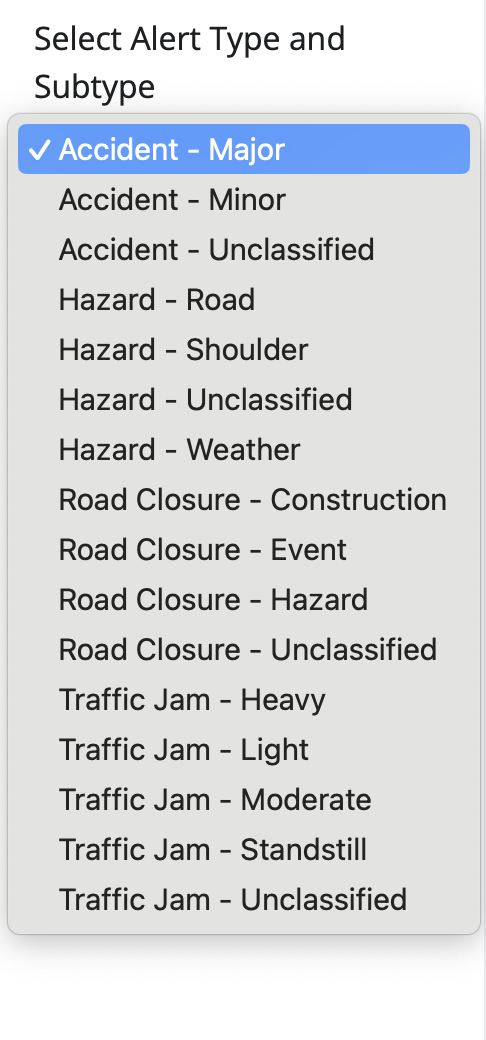
\includegraphics{./ps6/images/Dropdown Menu.png}

}

\caption{Dropdown menu showing type-subtype combinations}

\end{figure}%

\begin{enumerate}
\def\labelenumi{\alph{enumi}.}
\setcounter{enumi}{1}
\tightlist
\item
\end{enumerate}

\begin{figure}[H]

{\centering 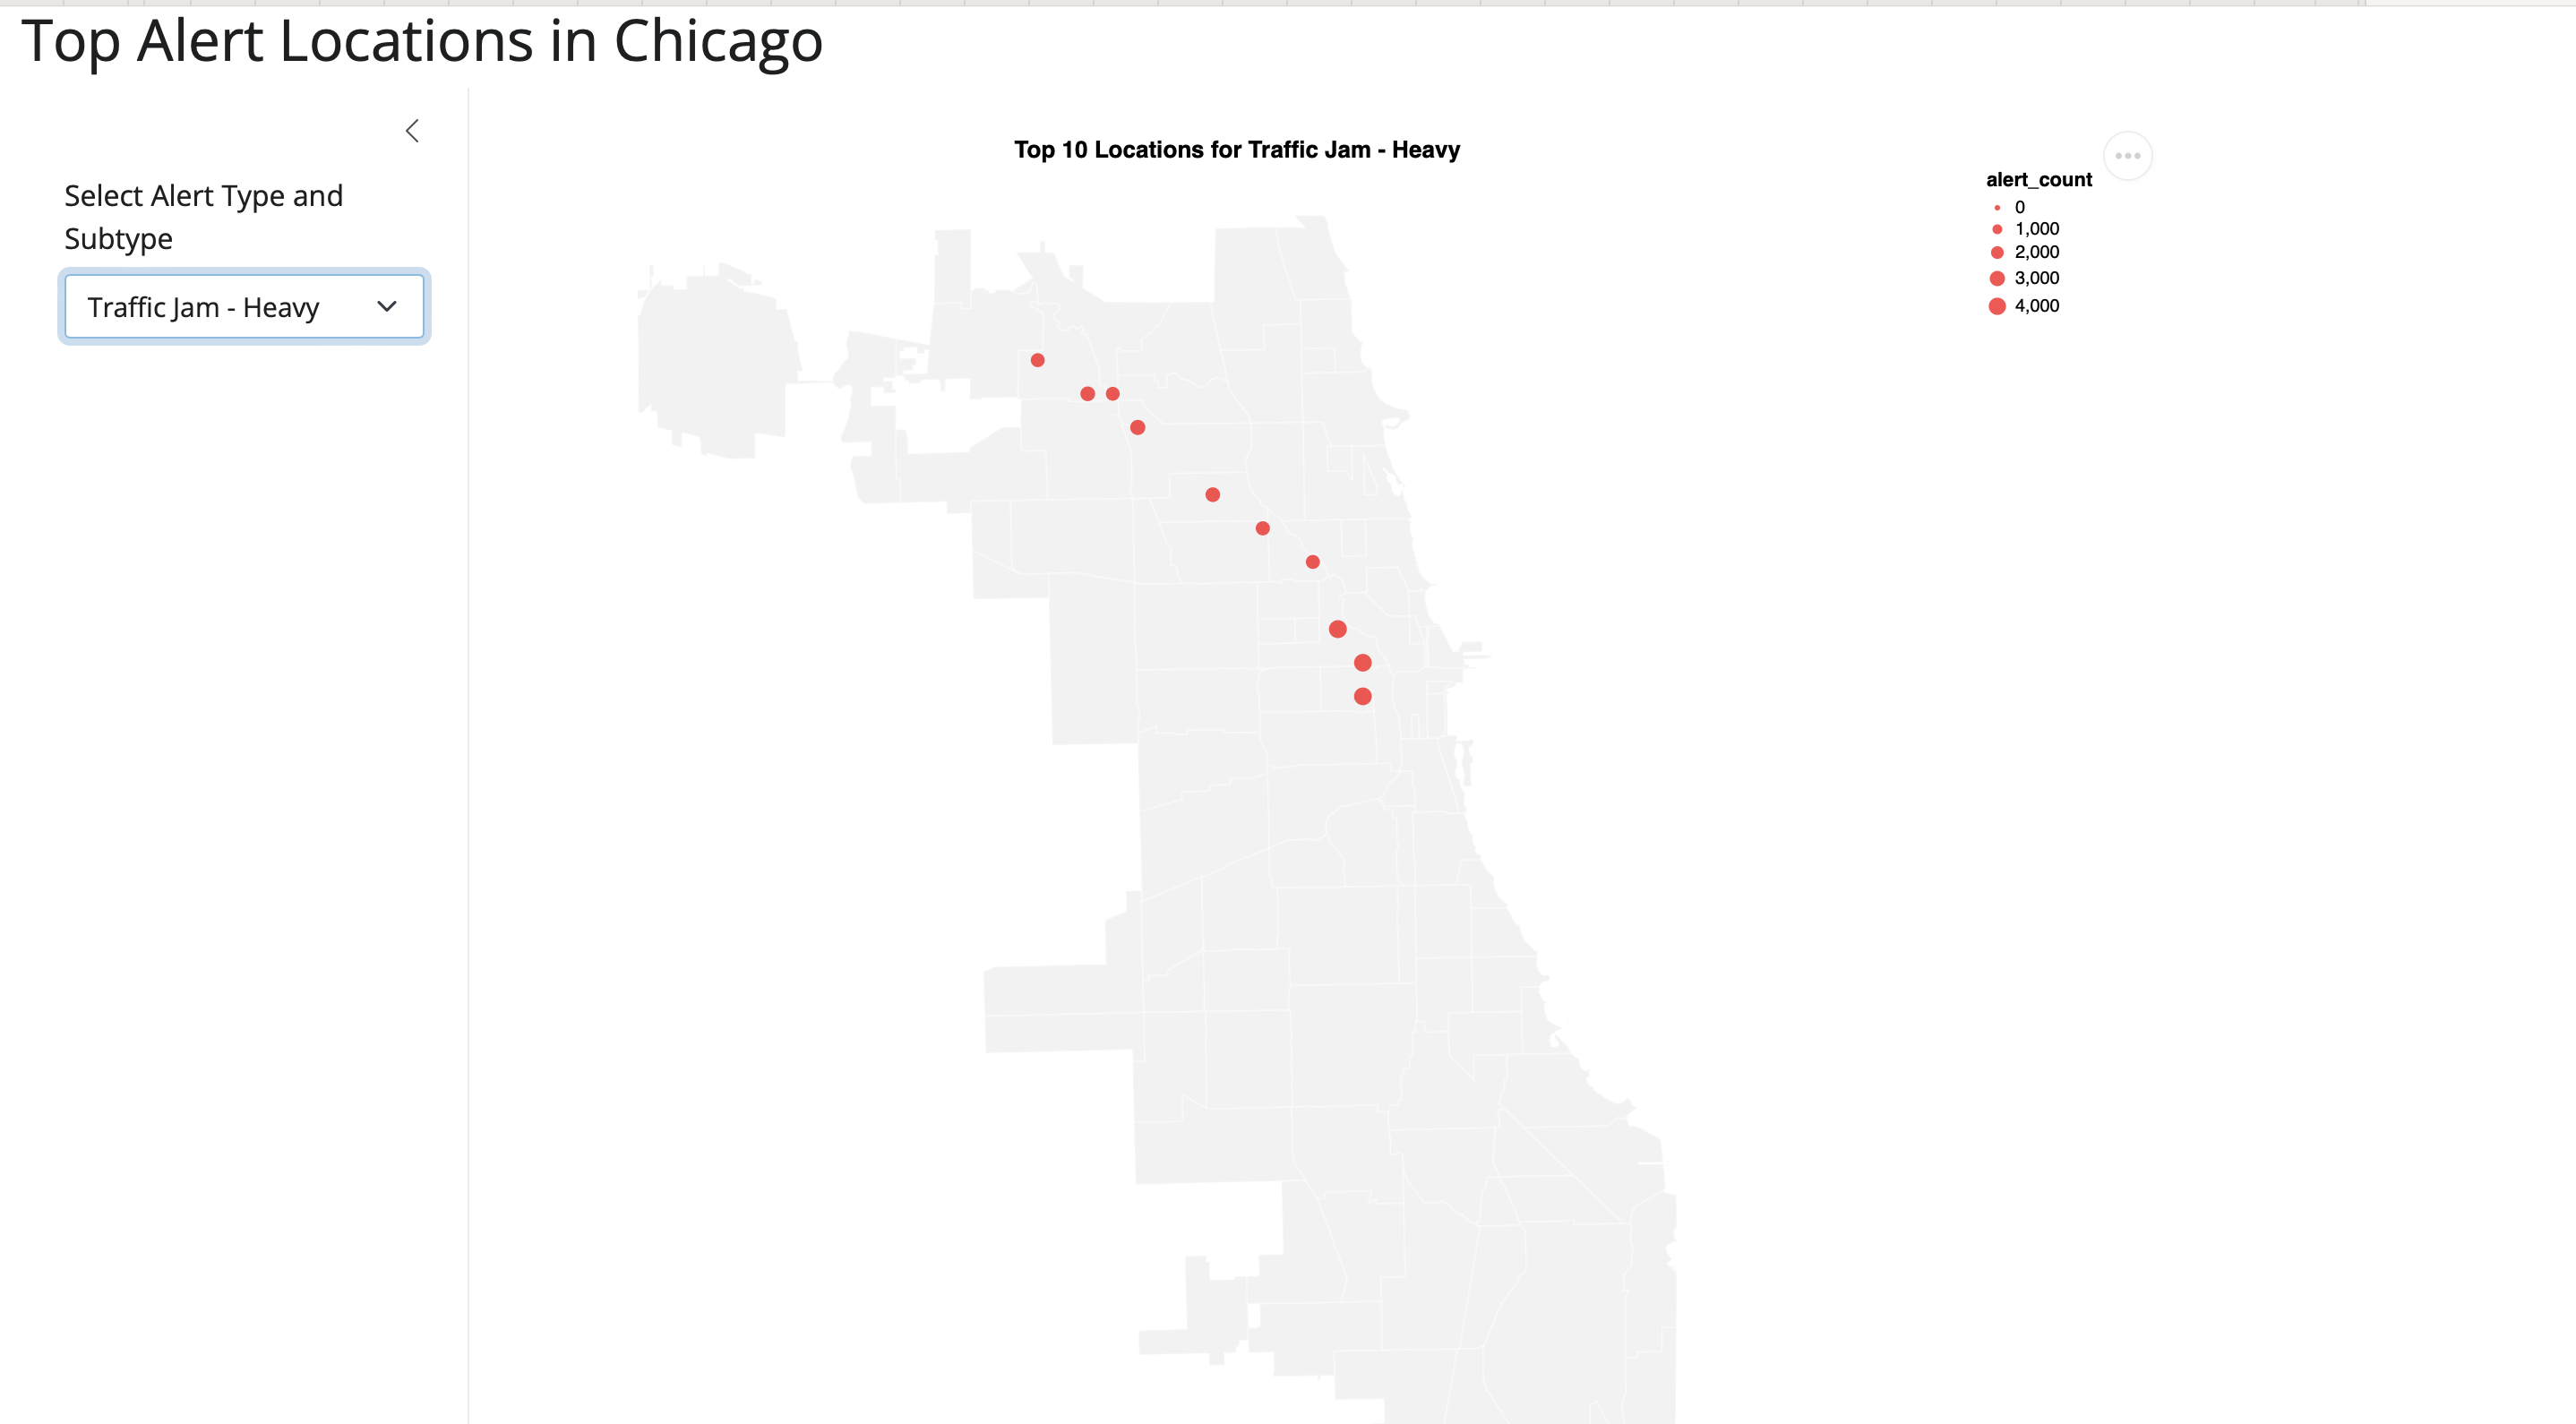
\includegraphics{.ps6/images/1.png}

}

\caption{Map showing top 10 locations for ``Traffic Jam - Heavy''}

\end{figure}%

The map above shows the top 10 locations where heavy traffic jams were
reported, with larger circles indicating more alerts at that location.

\begin{enumerate}
\def\labelenumi{\alph{enumi}.}
\setcounter{enumi}{2}
\tightlist
\item
\end{enumerate}

\begin{figure}[H]

{\centering 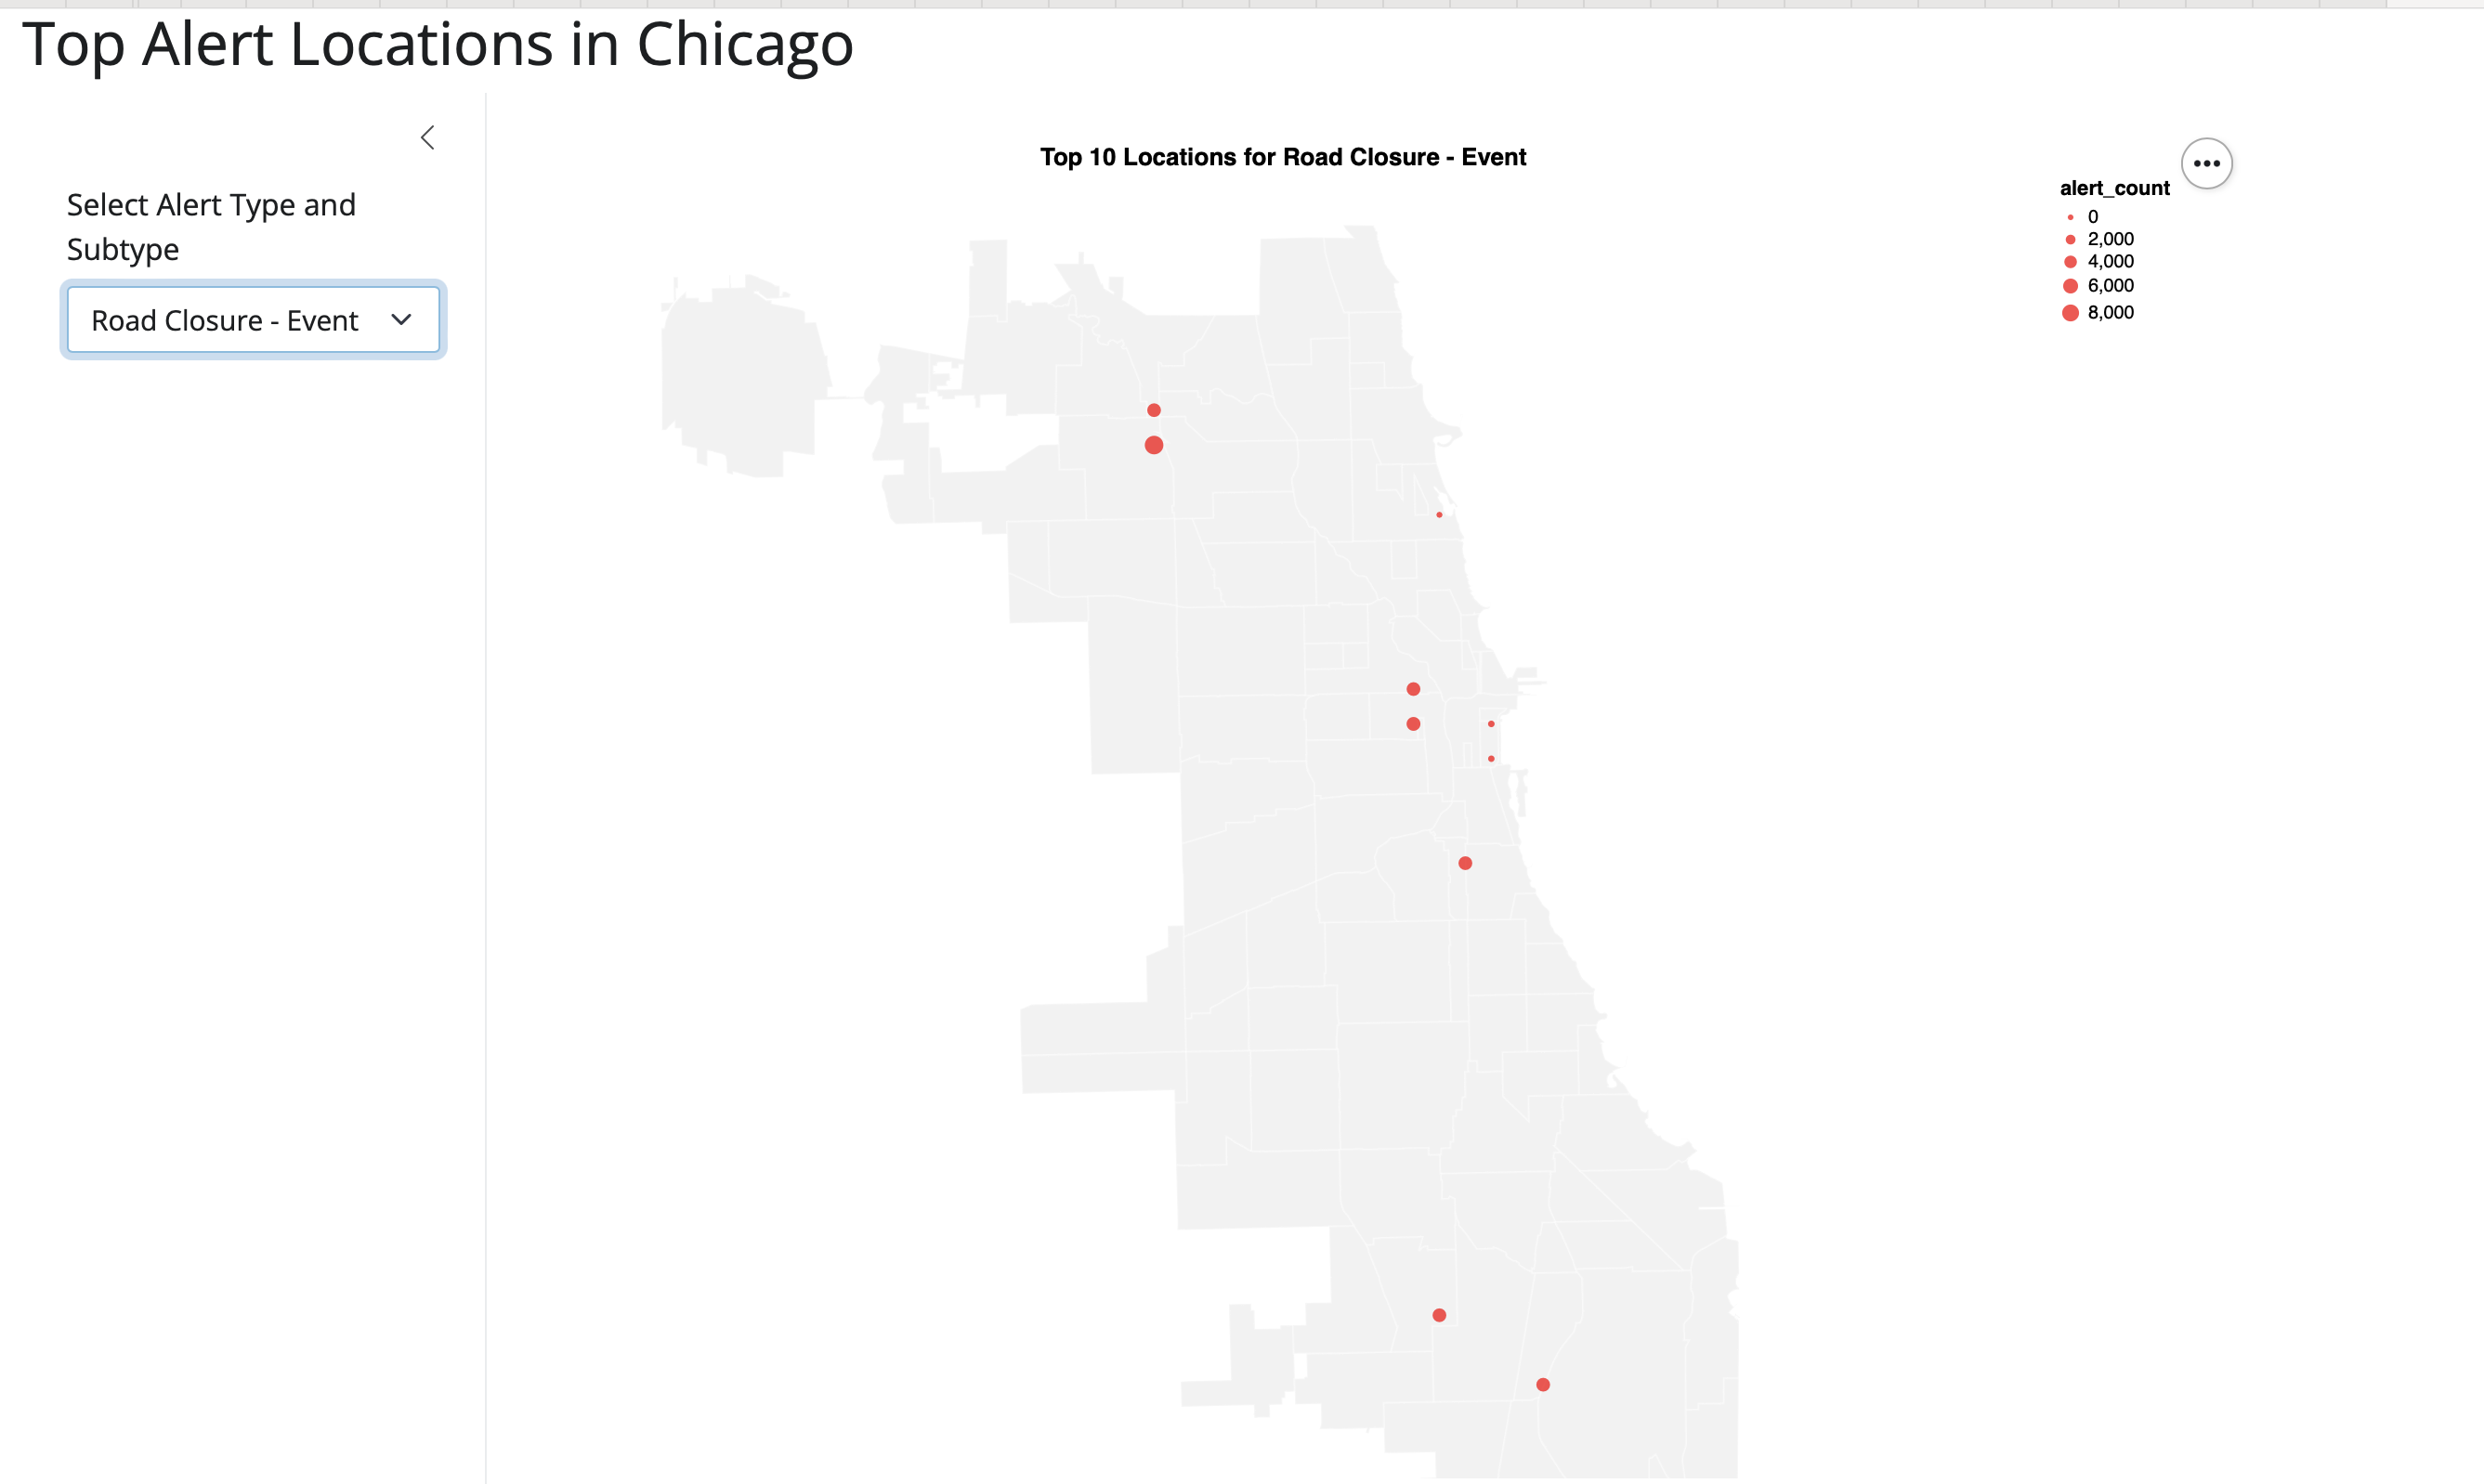
\includegraphics{.ps6/images/2.png}

}

\caption{Map showing most common location for road closure due to event}

\end{figure}%

latitude\_bin:41.96, longitude\_bin:-87.75 is the most common location
for road closure due to event.

\begin{enumerate}
\def\labelenumi{\alph{enumi}.}
\setcounter{enumi}{3}
\tightlist
\item
  What is the most common location for major accidents?
  latitude\_bin:41.9, longitude\_bin:-87.66 is the most common location
  for major accidents.
\end{enumerate}

\begin{figure}[H]

{\centering 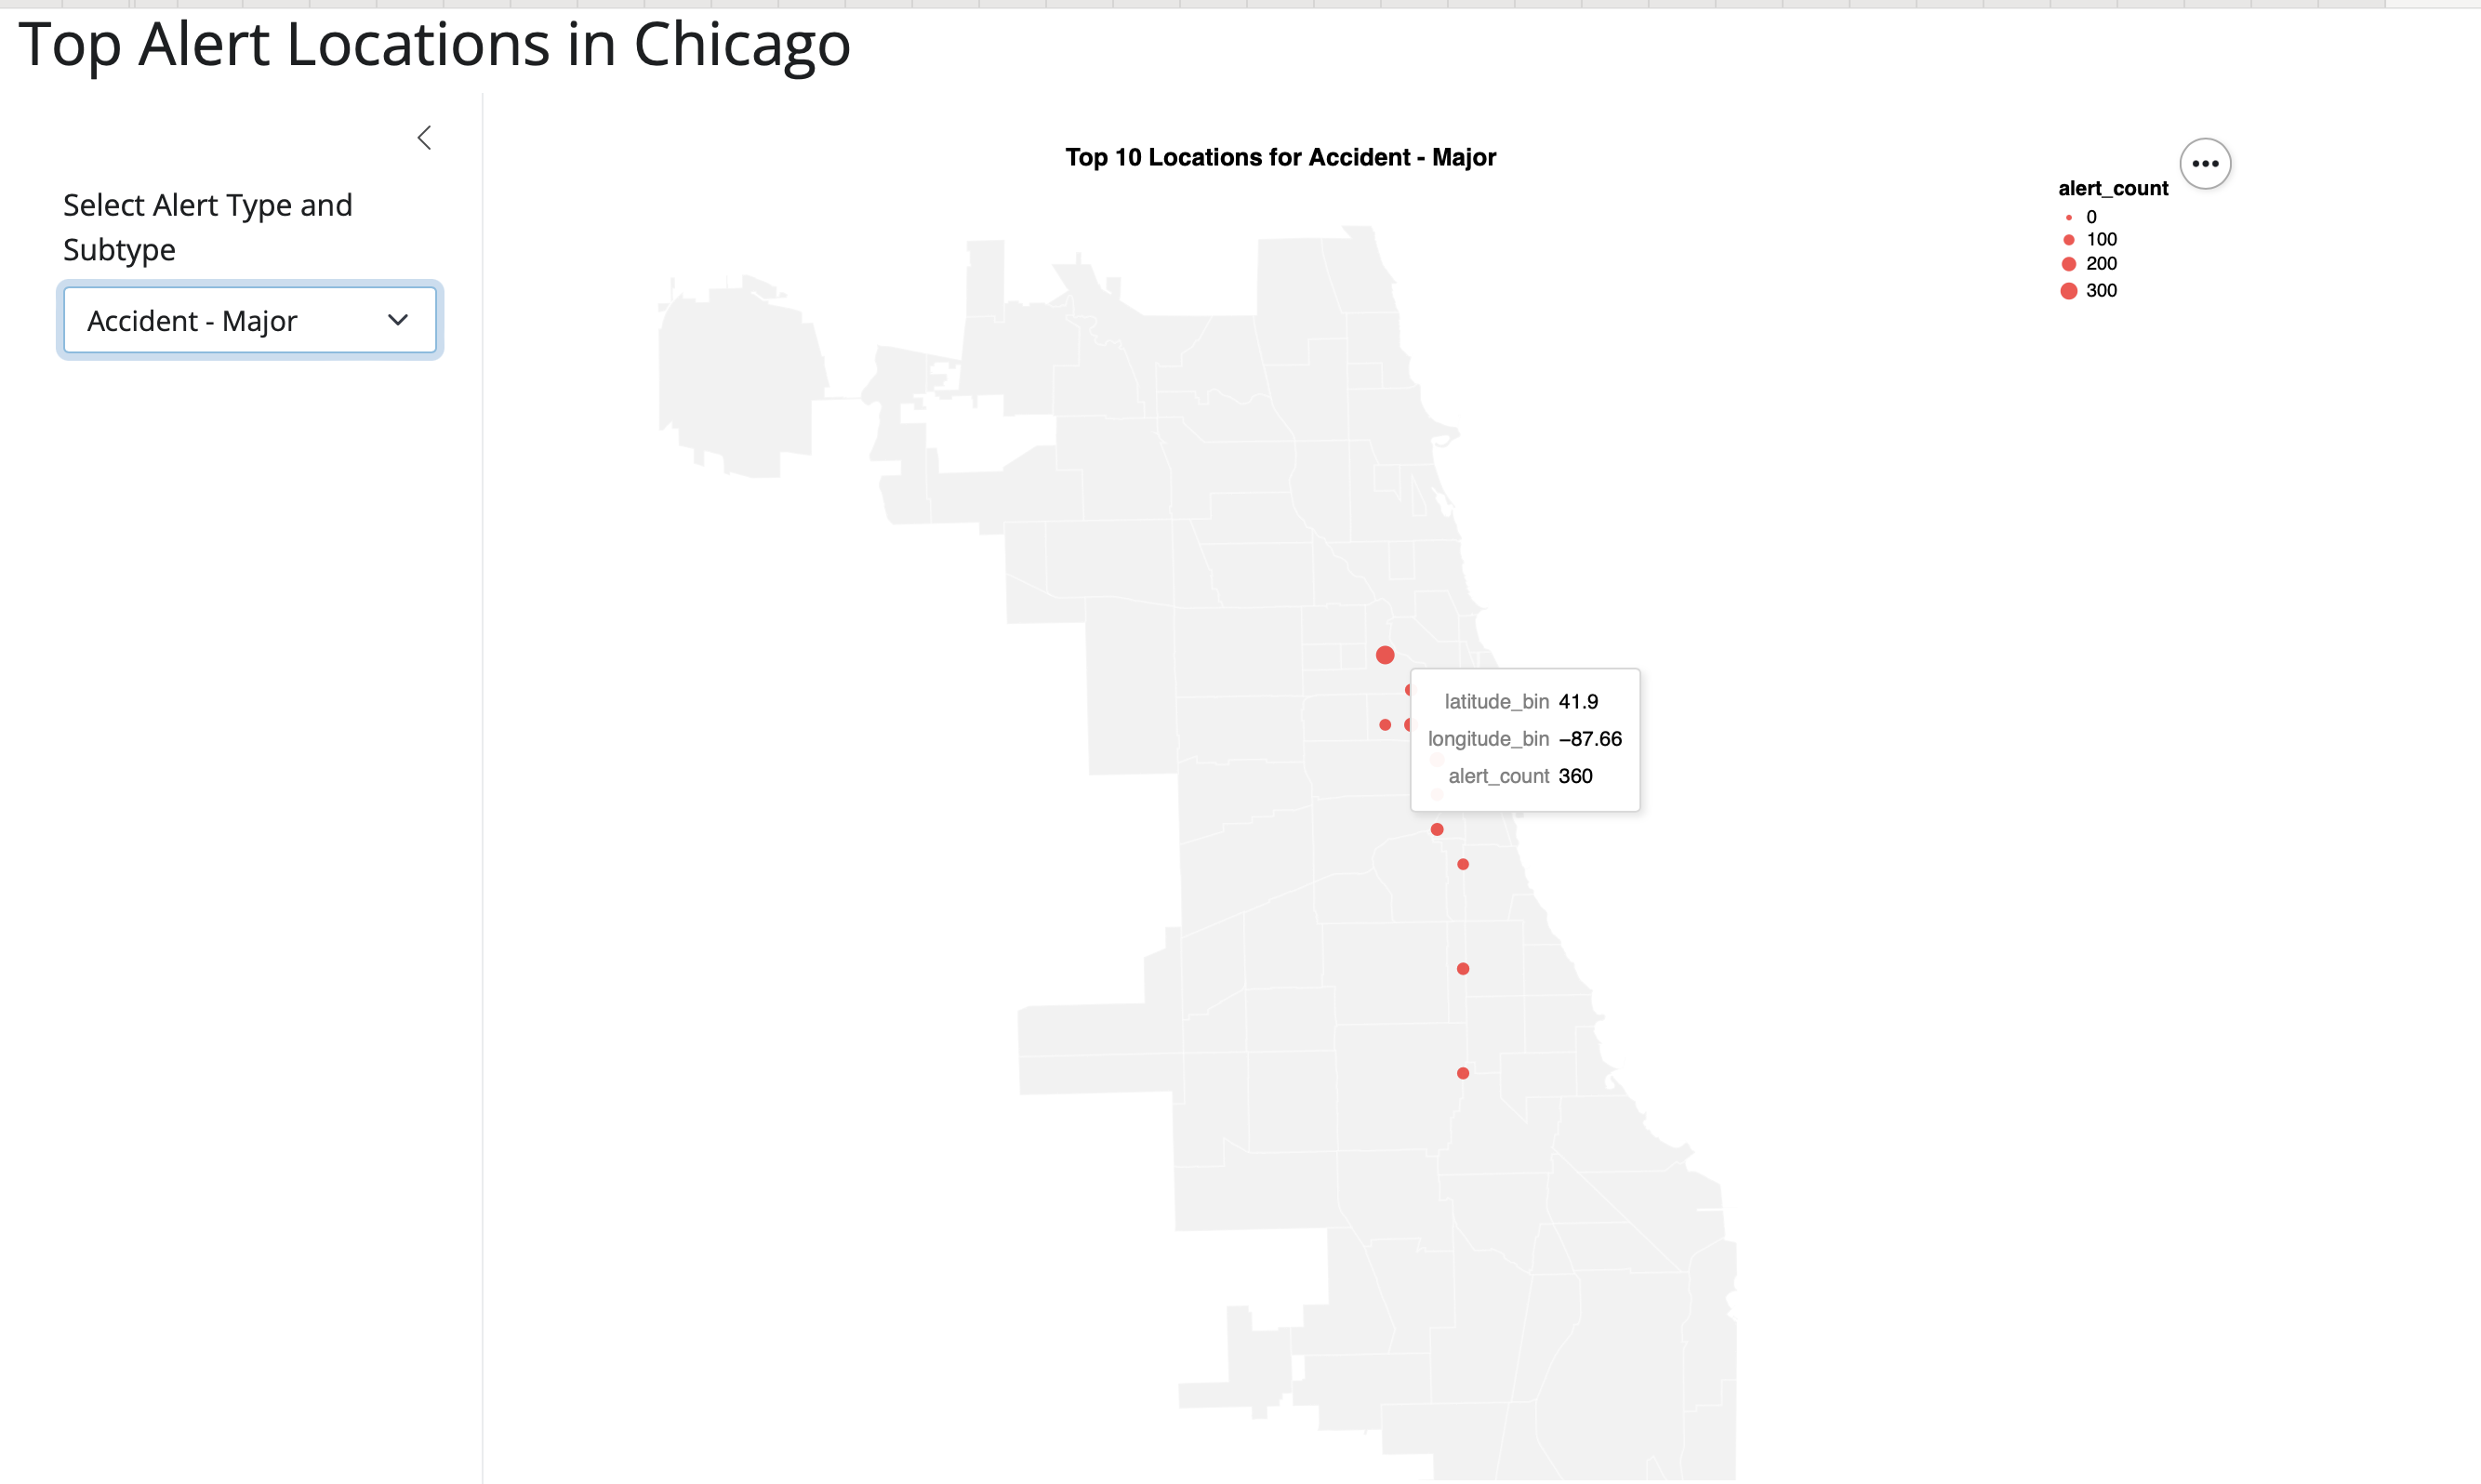
\includegraphics{.ps6/images/3.png}

}

\caption{Map showing most common location for major accidents}

\end{figure}%

\begin{enumerate}
\def\labelenumi{\alph{enumi}.}
\setcounter{enumi}{4}
\tightlist
\item
  I suggest adding a reliability score column to enhance the dashboard.
  Since our dataset includes both \texttt{reliability} and
  \texttt{confidence} metrics, this addition would help users filter
  alerts based on their trustworthiness. For example, when analyzing
  traffic jams, users could focus on high-reliability reports (e.g.,
  those with multiple thumbs-up and high confidence scores), making
  their route planning more dependable. This feature would be
  particularly useful during rush hours when accurate traffic
  information is crucial. The reliability score could be displayed using
  color intensity on the map, making it visually intuitive to identify
  the most reliable alerts.
\end{enumerate}

\section*{App \#2: Top Location by Alert Type and Hour Dashboard (20
points)}\label{app-2-top-location-by-alert-type-and-hour-dashboard-20-points}
\addcontentsline{toc}{section}{App \#2: Top Location by Alert Type and
Hour Dashboard (20 points)}

\begin{enumerate}
\def\labelenumi{\arabic{enumi}.}
\tightlist
\item
\end{enumerate}

\begin{enumerate}
\def\labelenumi{\alph{enumi}.}
\item
  Given the timestamp format in our dataset (e.g., ``2024-02-04 16:40:41
  UTC''), it would not be a good idea to collapse the dataset directly
  by the ts column. The timestamps contain very detailed information
  including year, month, day, hours, minutes, and seconds in UTC format.
  Since our goal is to analyze traffic patterns by hour of the day,
  collapsing by the exact timestamp would create unnecessary
  fragmentation of the data, where similar events occurring at slightly
  different times (like 16:40:41 and 16:41:00) would be treated as
  separate groups. Instead, it would be more meaningful to extract just
  the hour component from these timestamps, allowing us to aggregate
  traffic patterns into 24 hourly slots that better represent daily
  traffic trends.
\item
\end{enumerate}

Saved hourly aggregation data with 62825 rows.

\begin{enumerate}
\def\labelenumi{\alph{enumi}.}
\setcounter{enumi}{2}
\tightlist
\item
\end{enumerate}

\begin{enumerate}
\def\labelenumi{\arabic{enumi}.}
\setcounter{enumi}{1}
\tightlist
\item
\end{enumerate}

\begin{enumerate}
\def\labelenumi{\alph{enumi}.}
\item
  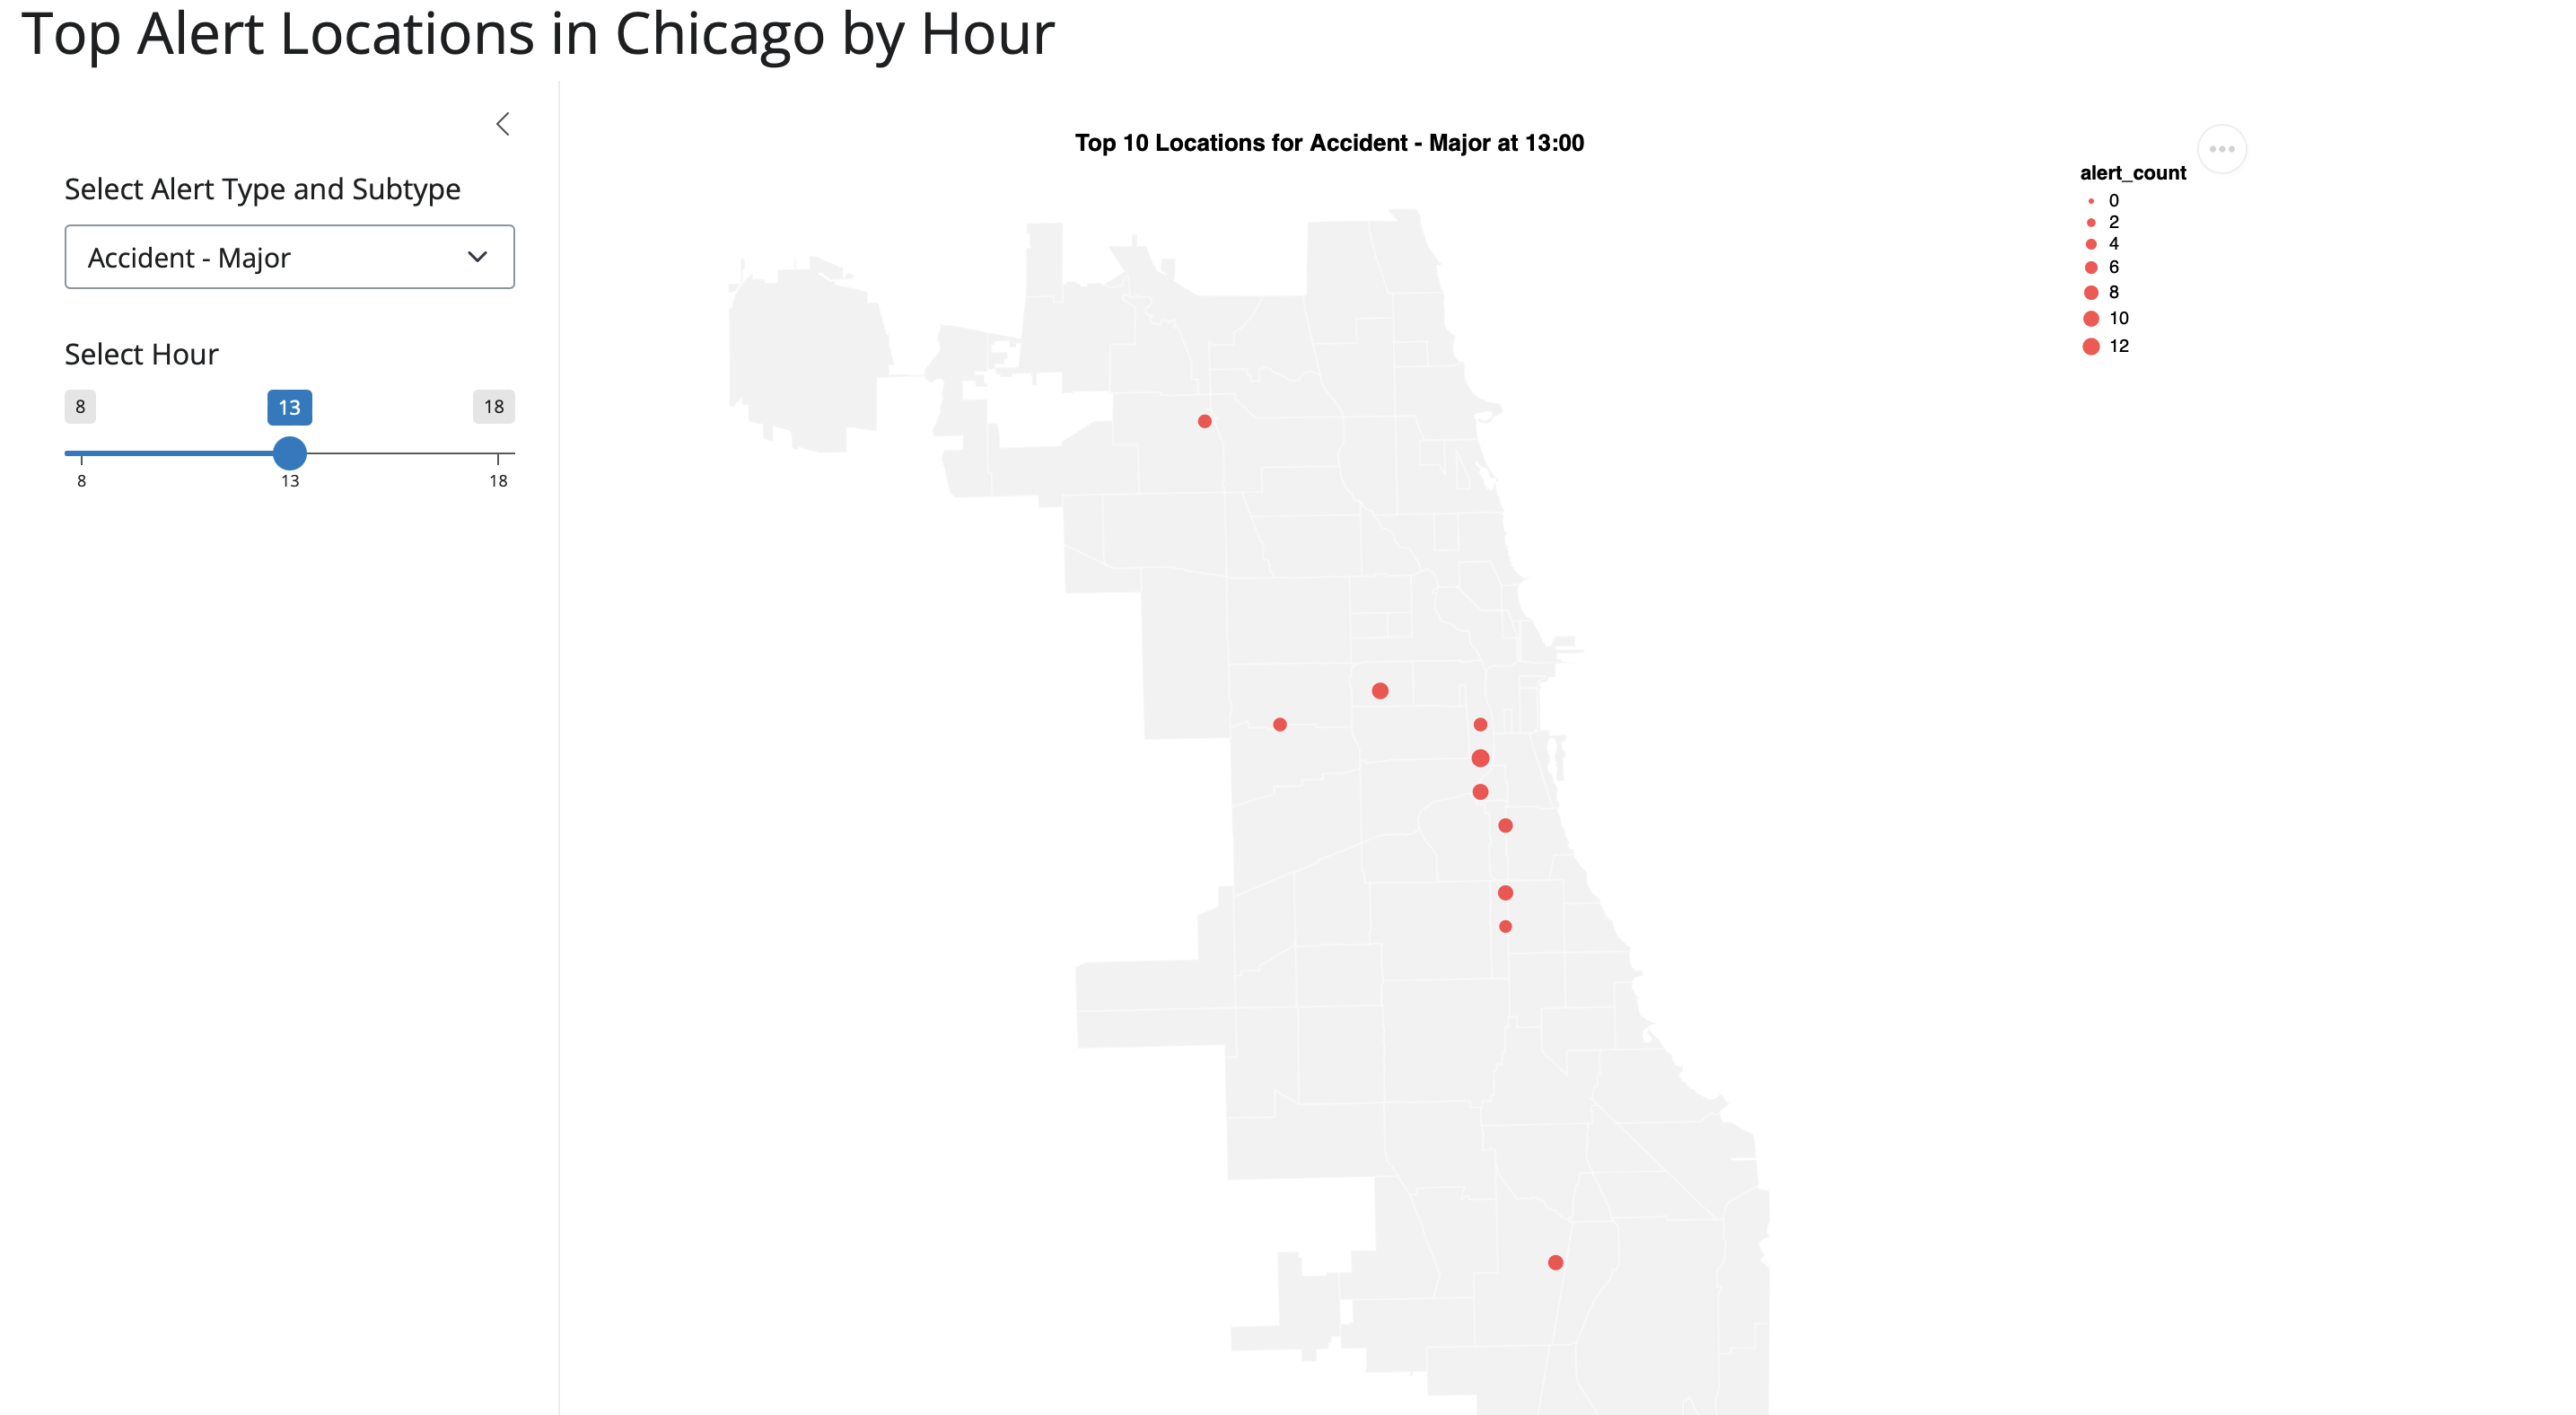
\includegraphics{.ps6/images/4.png}
  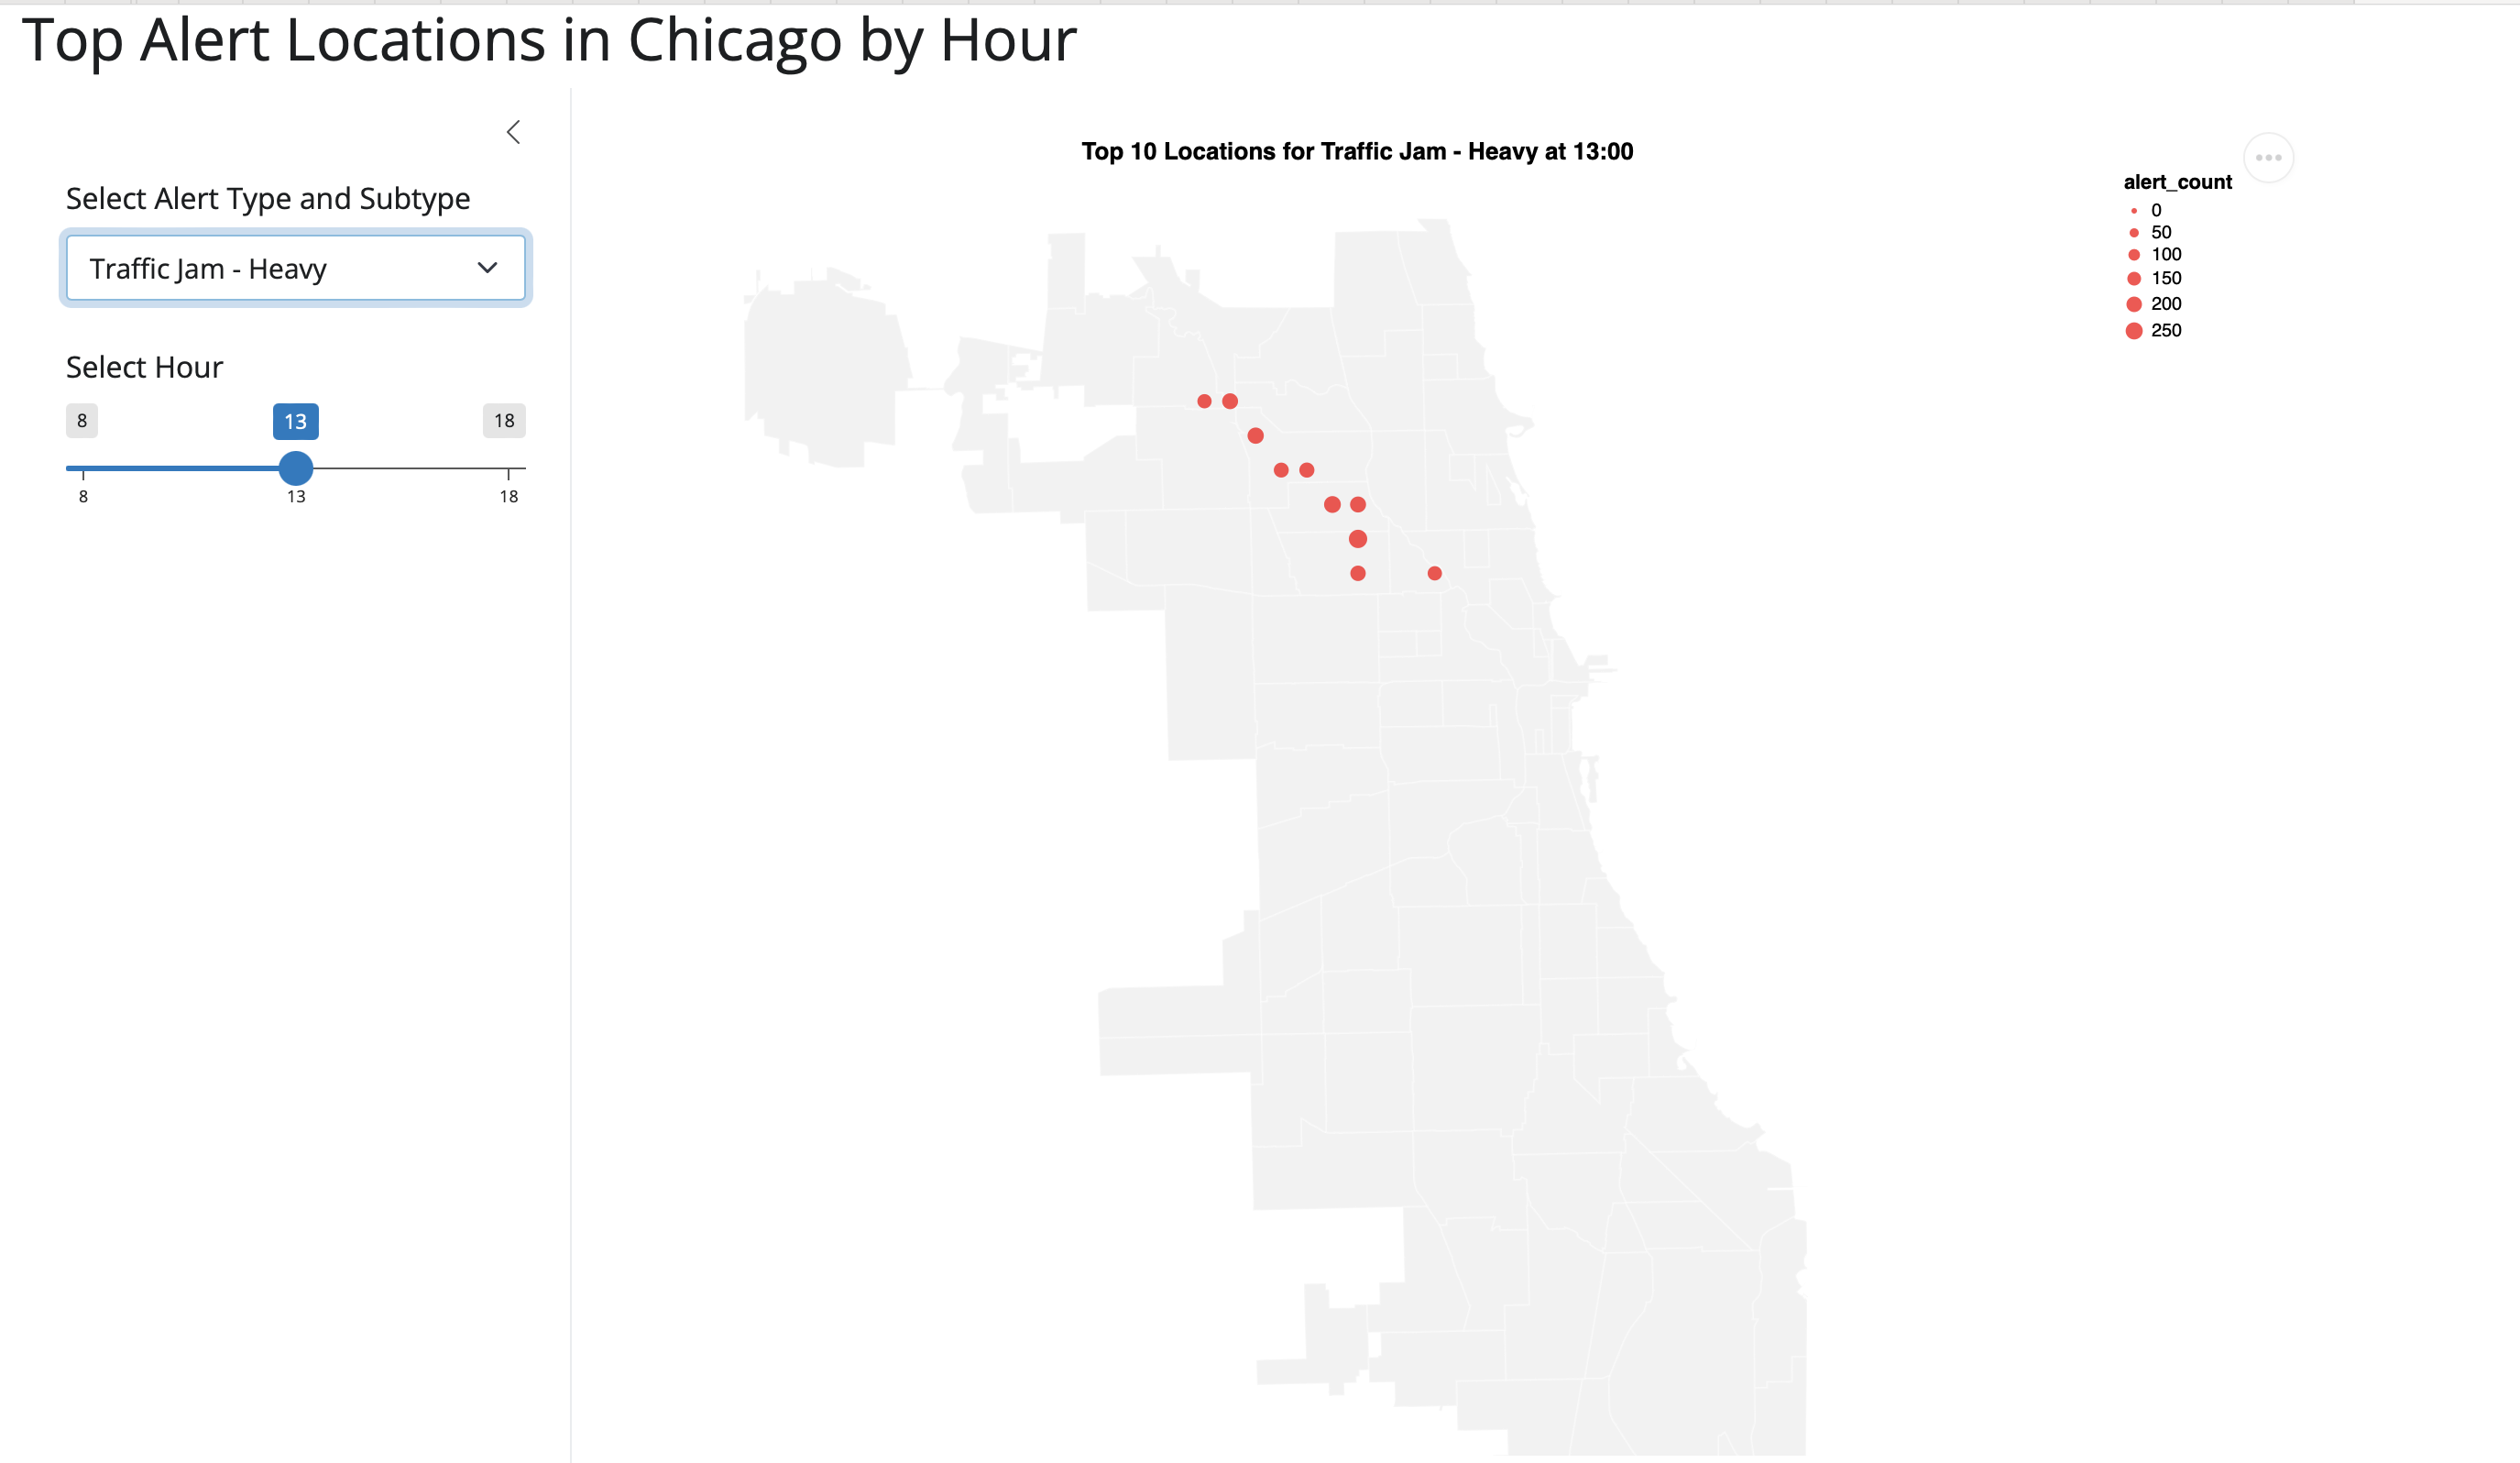
\includegraphics{.ps6/images/5.png}
\item
  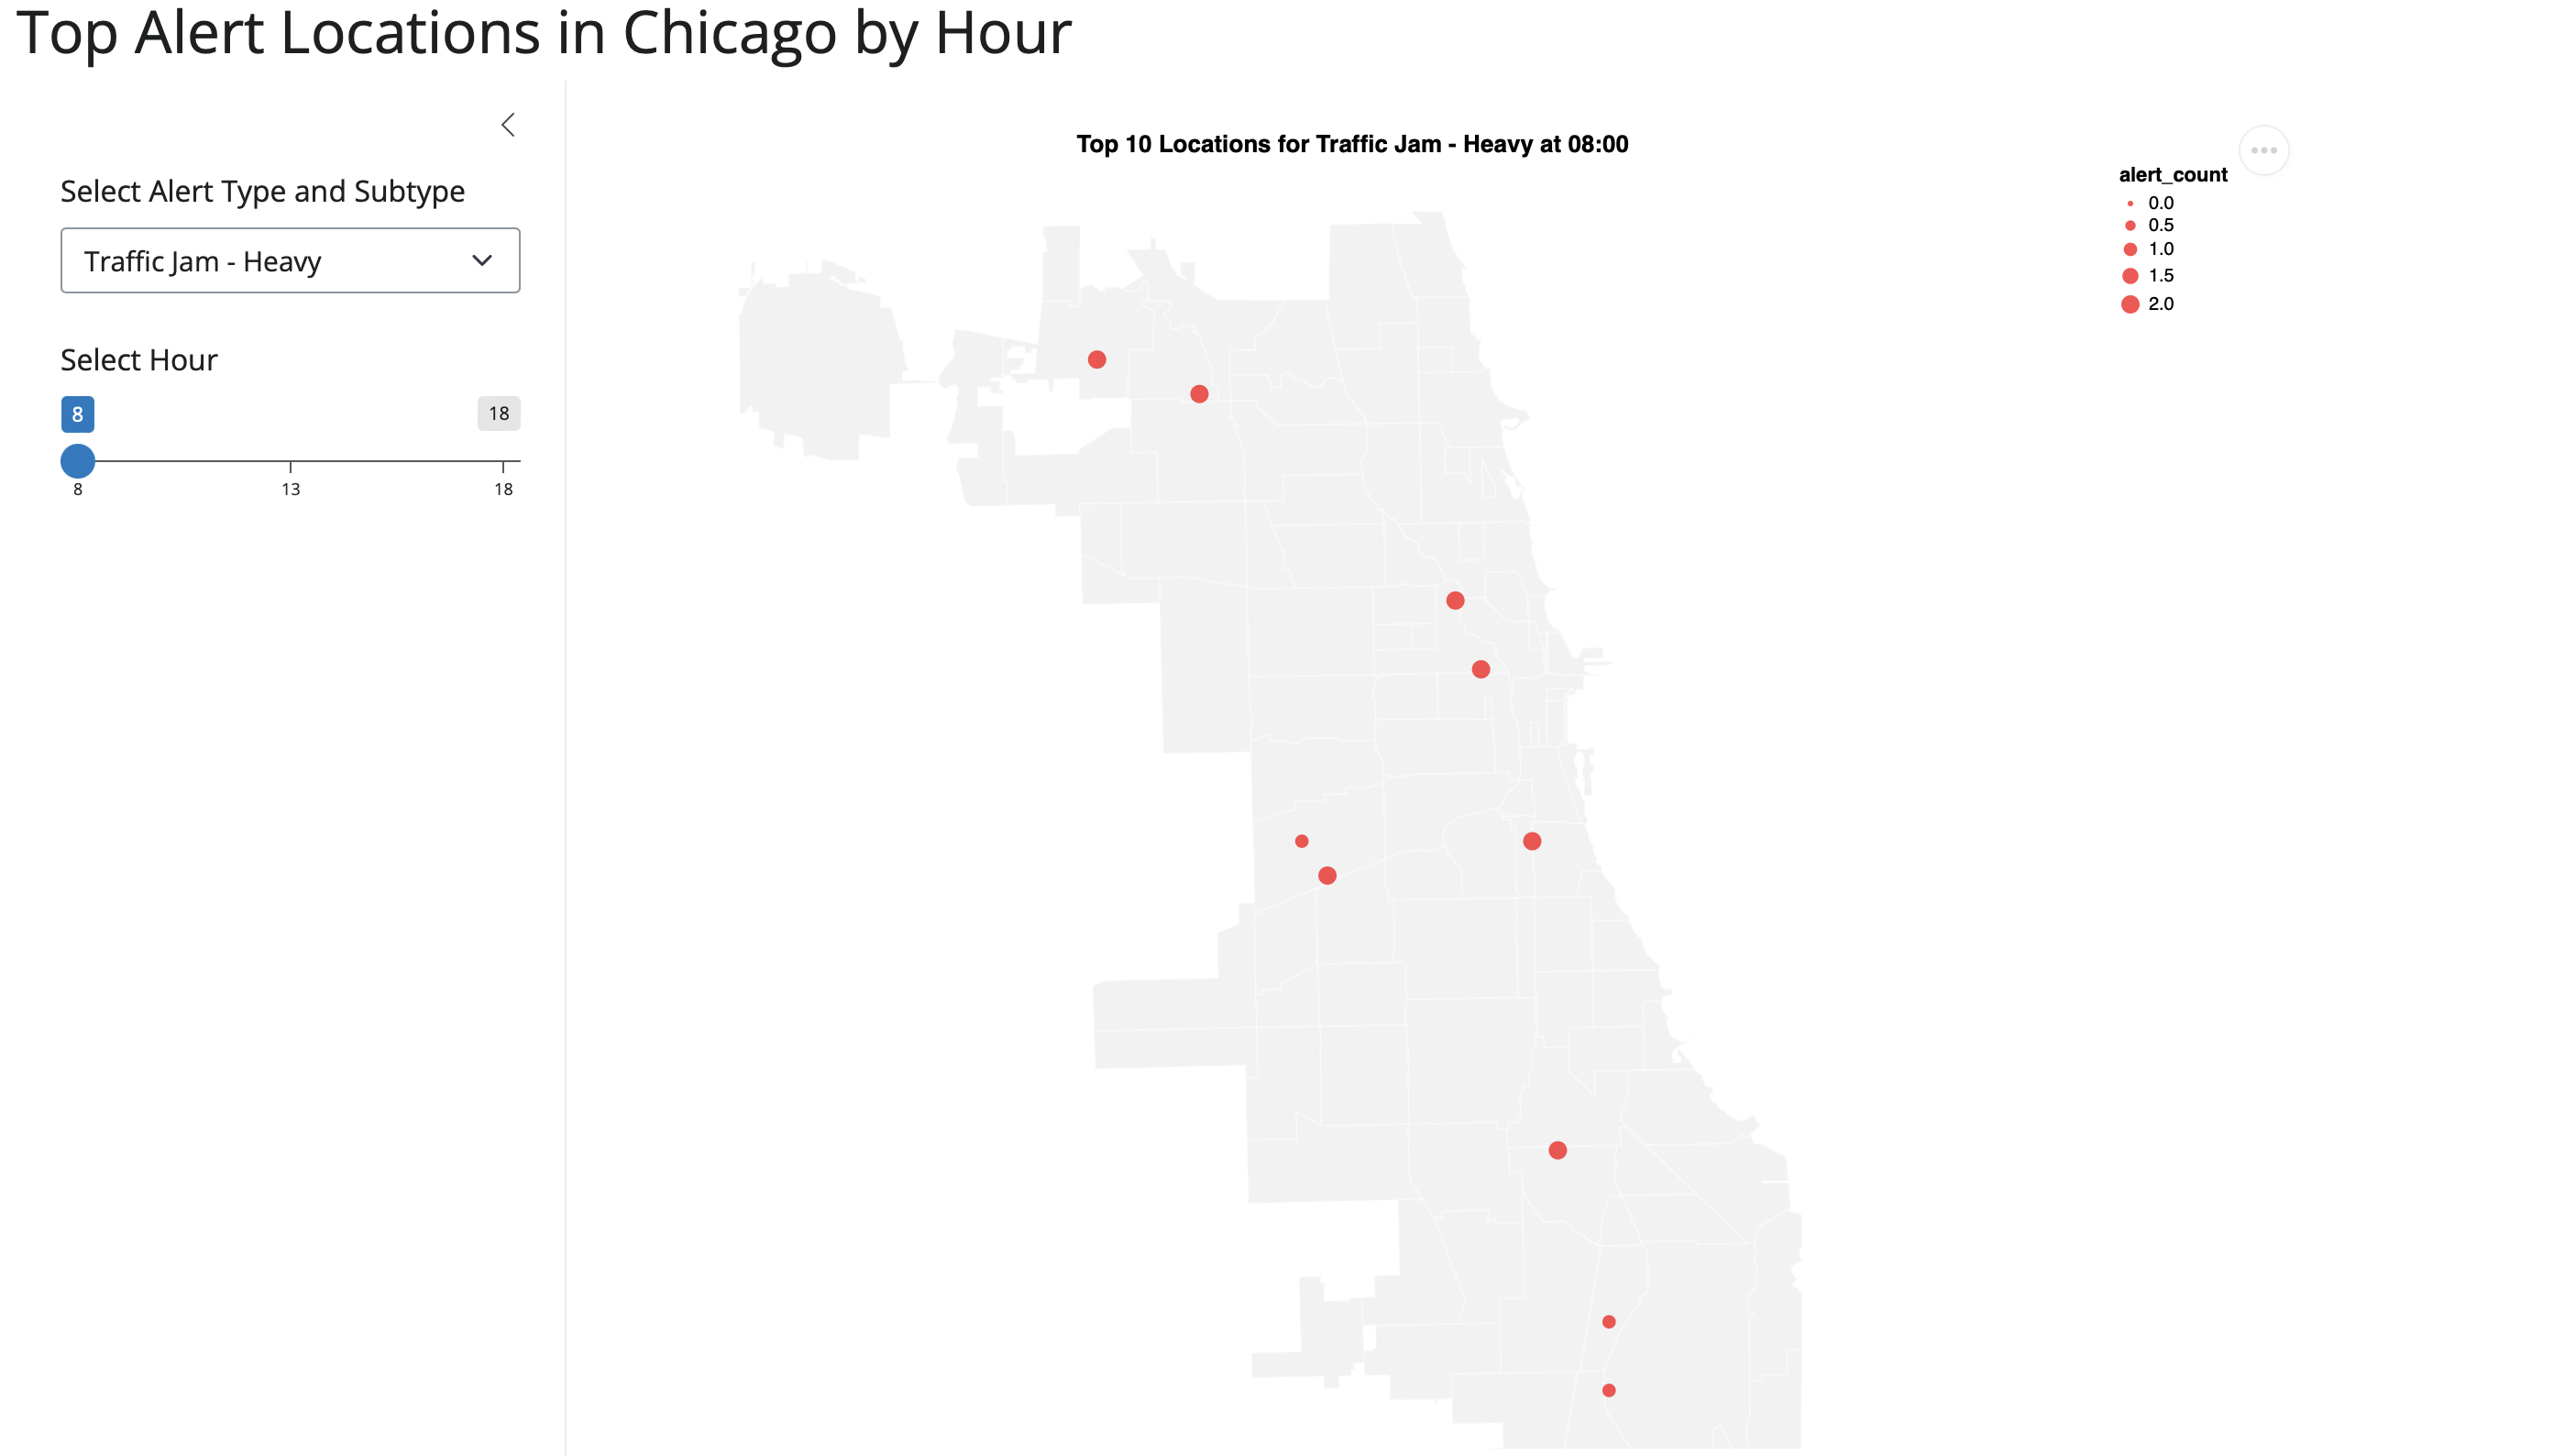
\includegraphics{.ps6/images/8.png}
  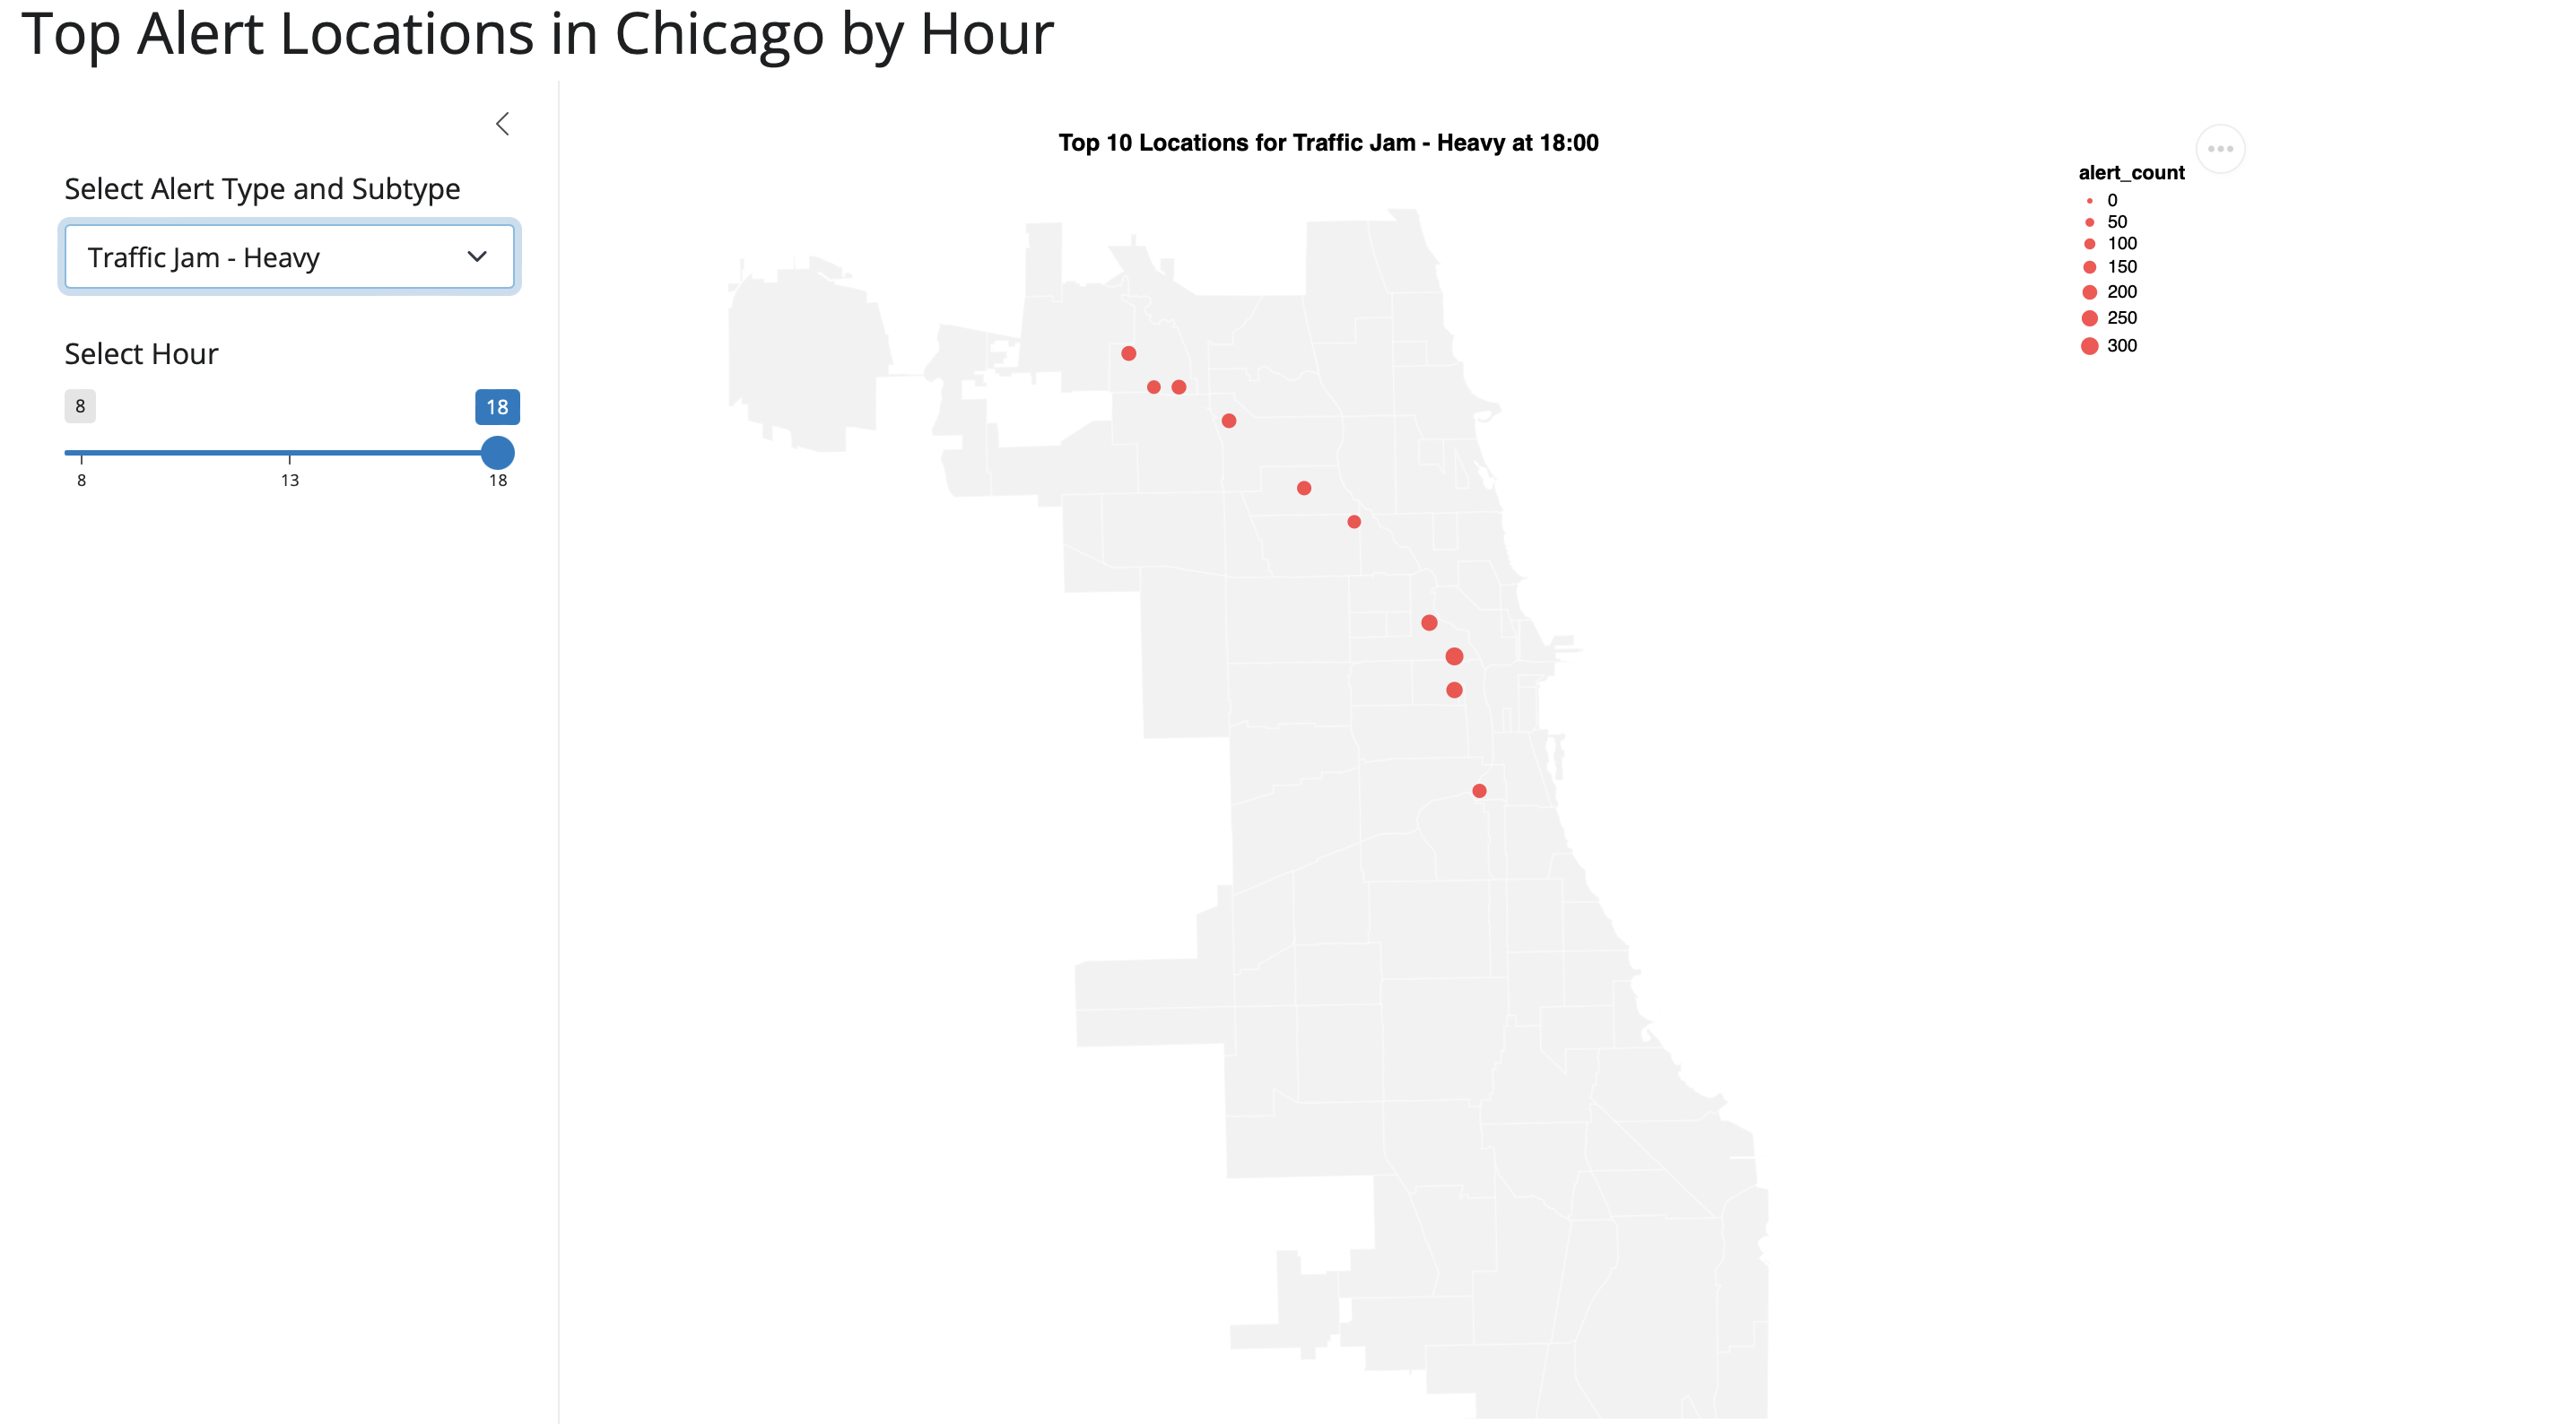
\includegraphics{.ps6/images/9.png}
  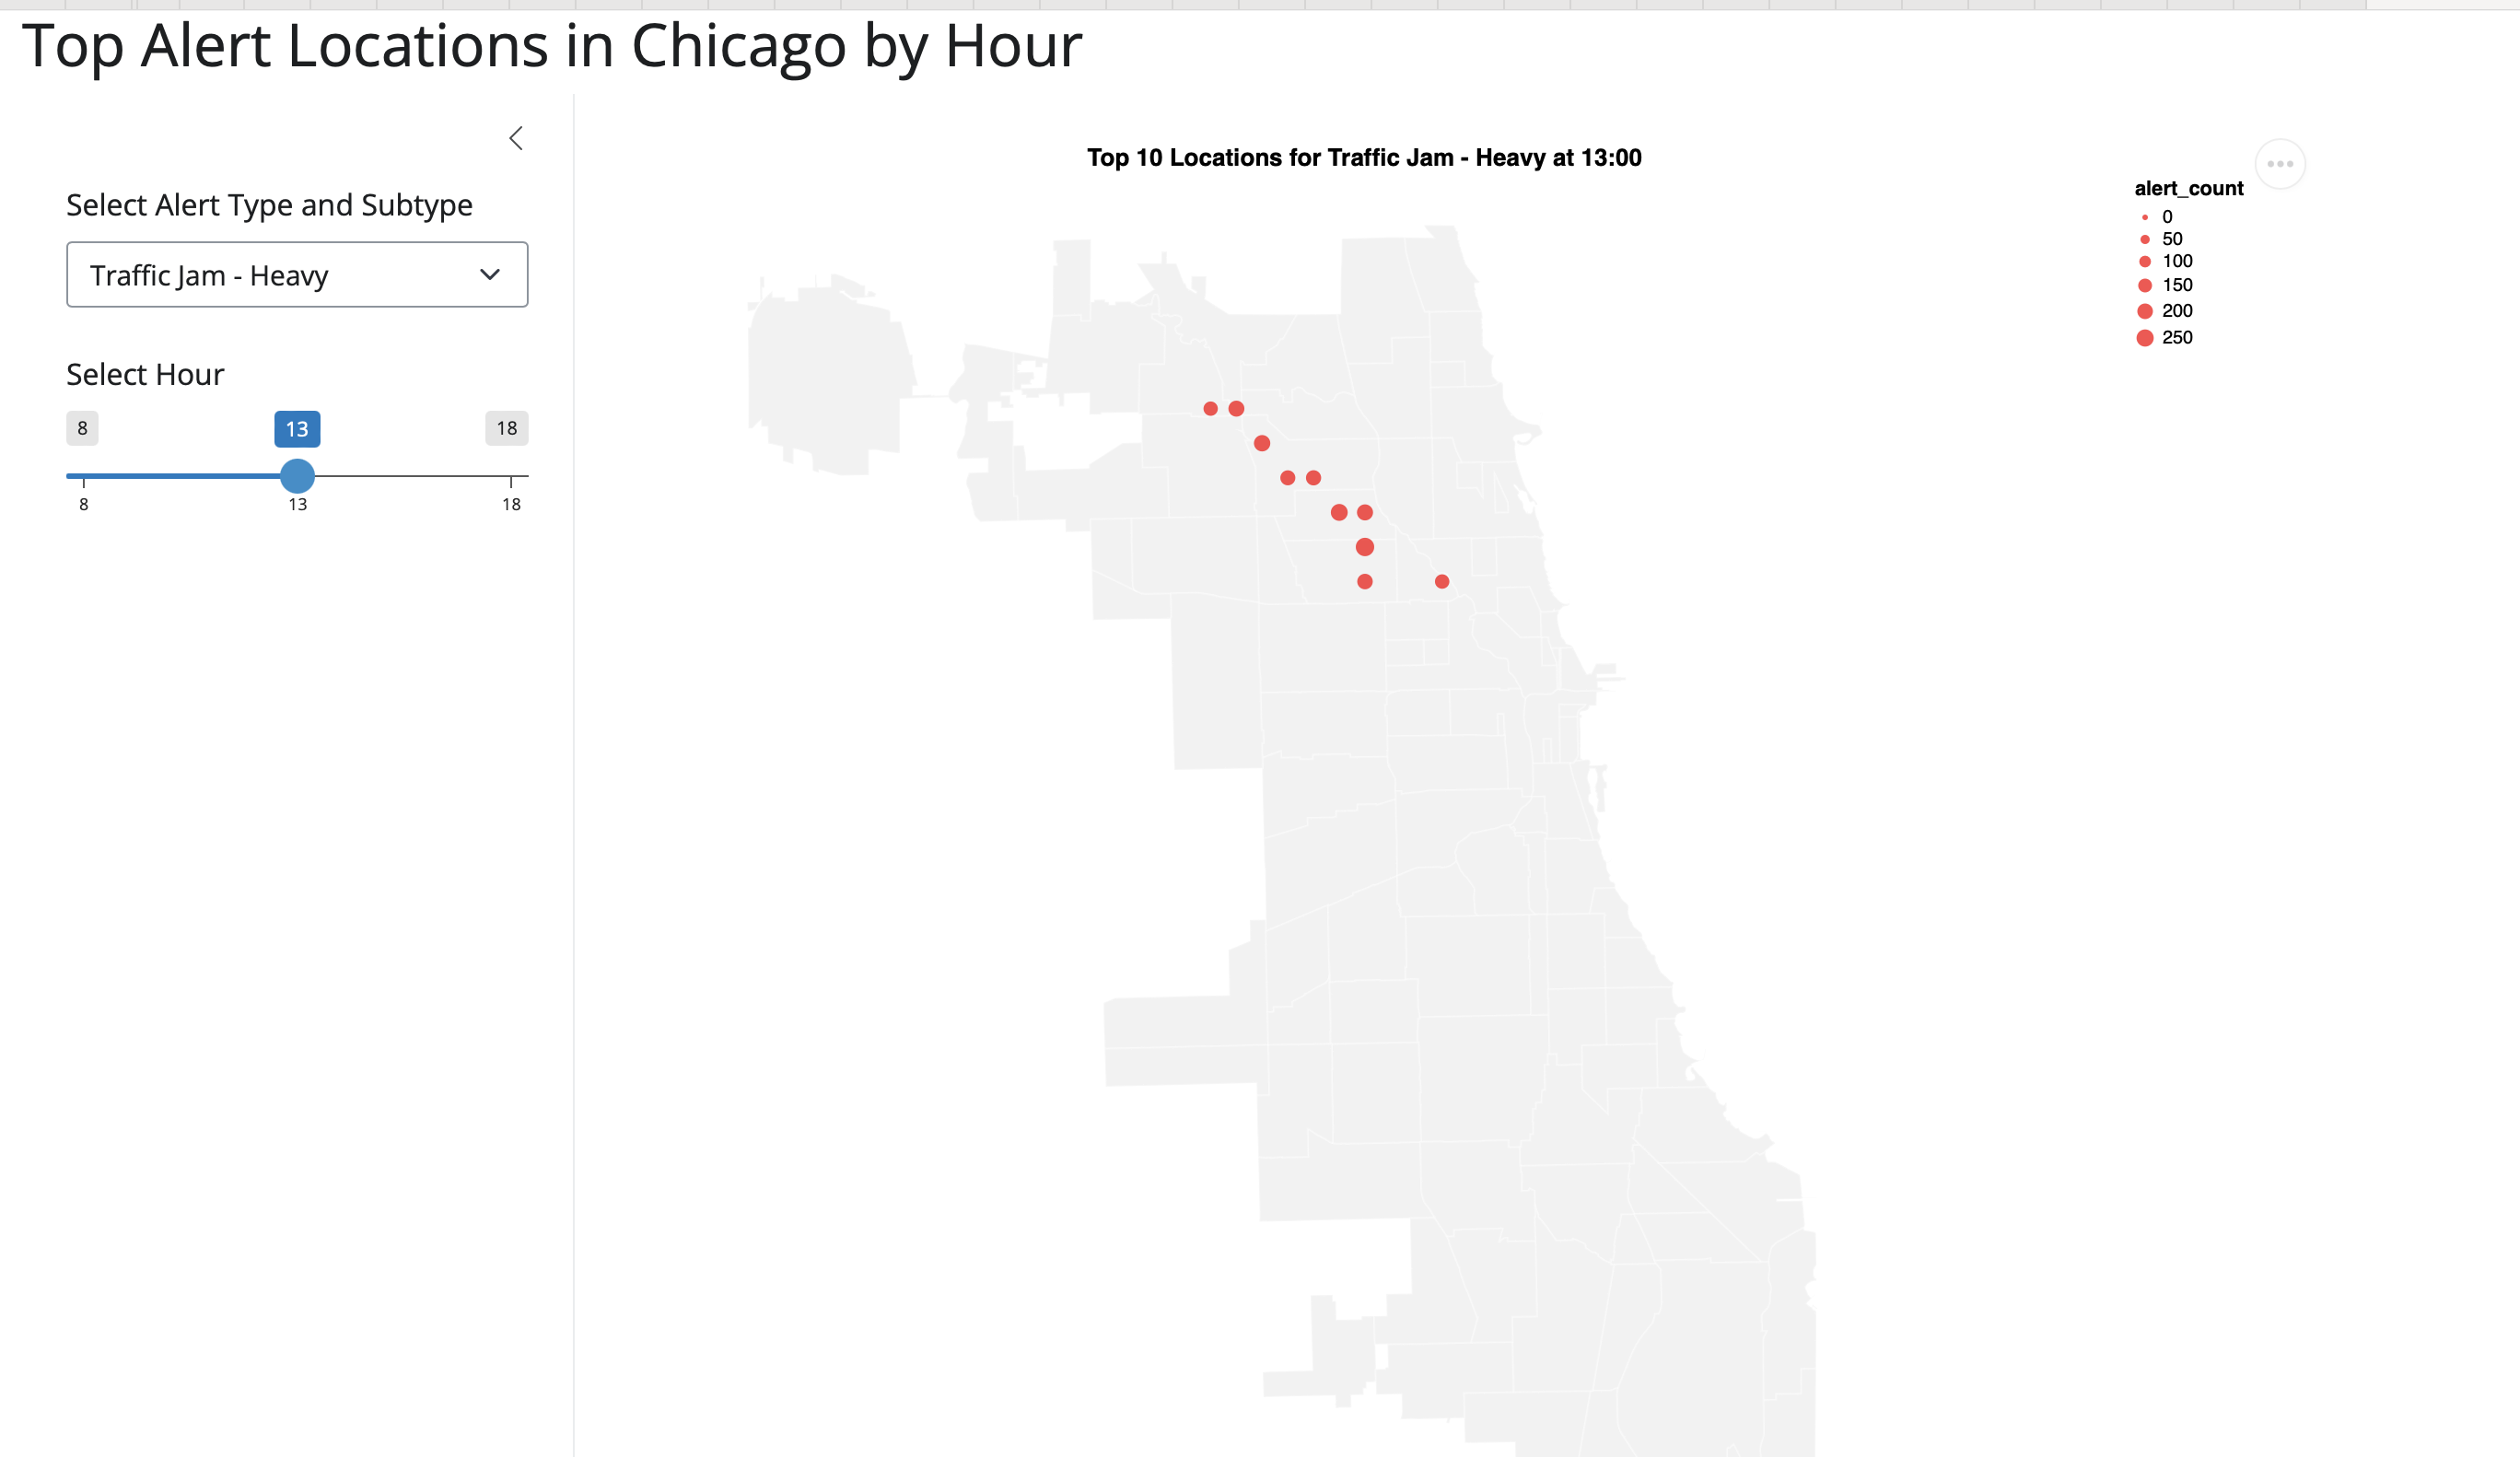
\includegraphics{.ps6/images/10.png}
\item
  The road construction is done more in evening hours from the map.
  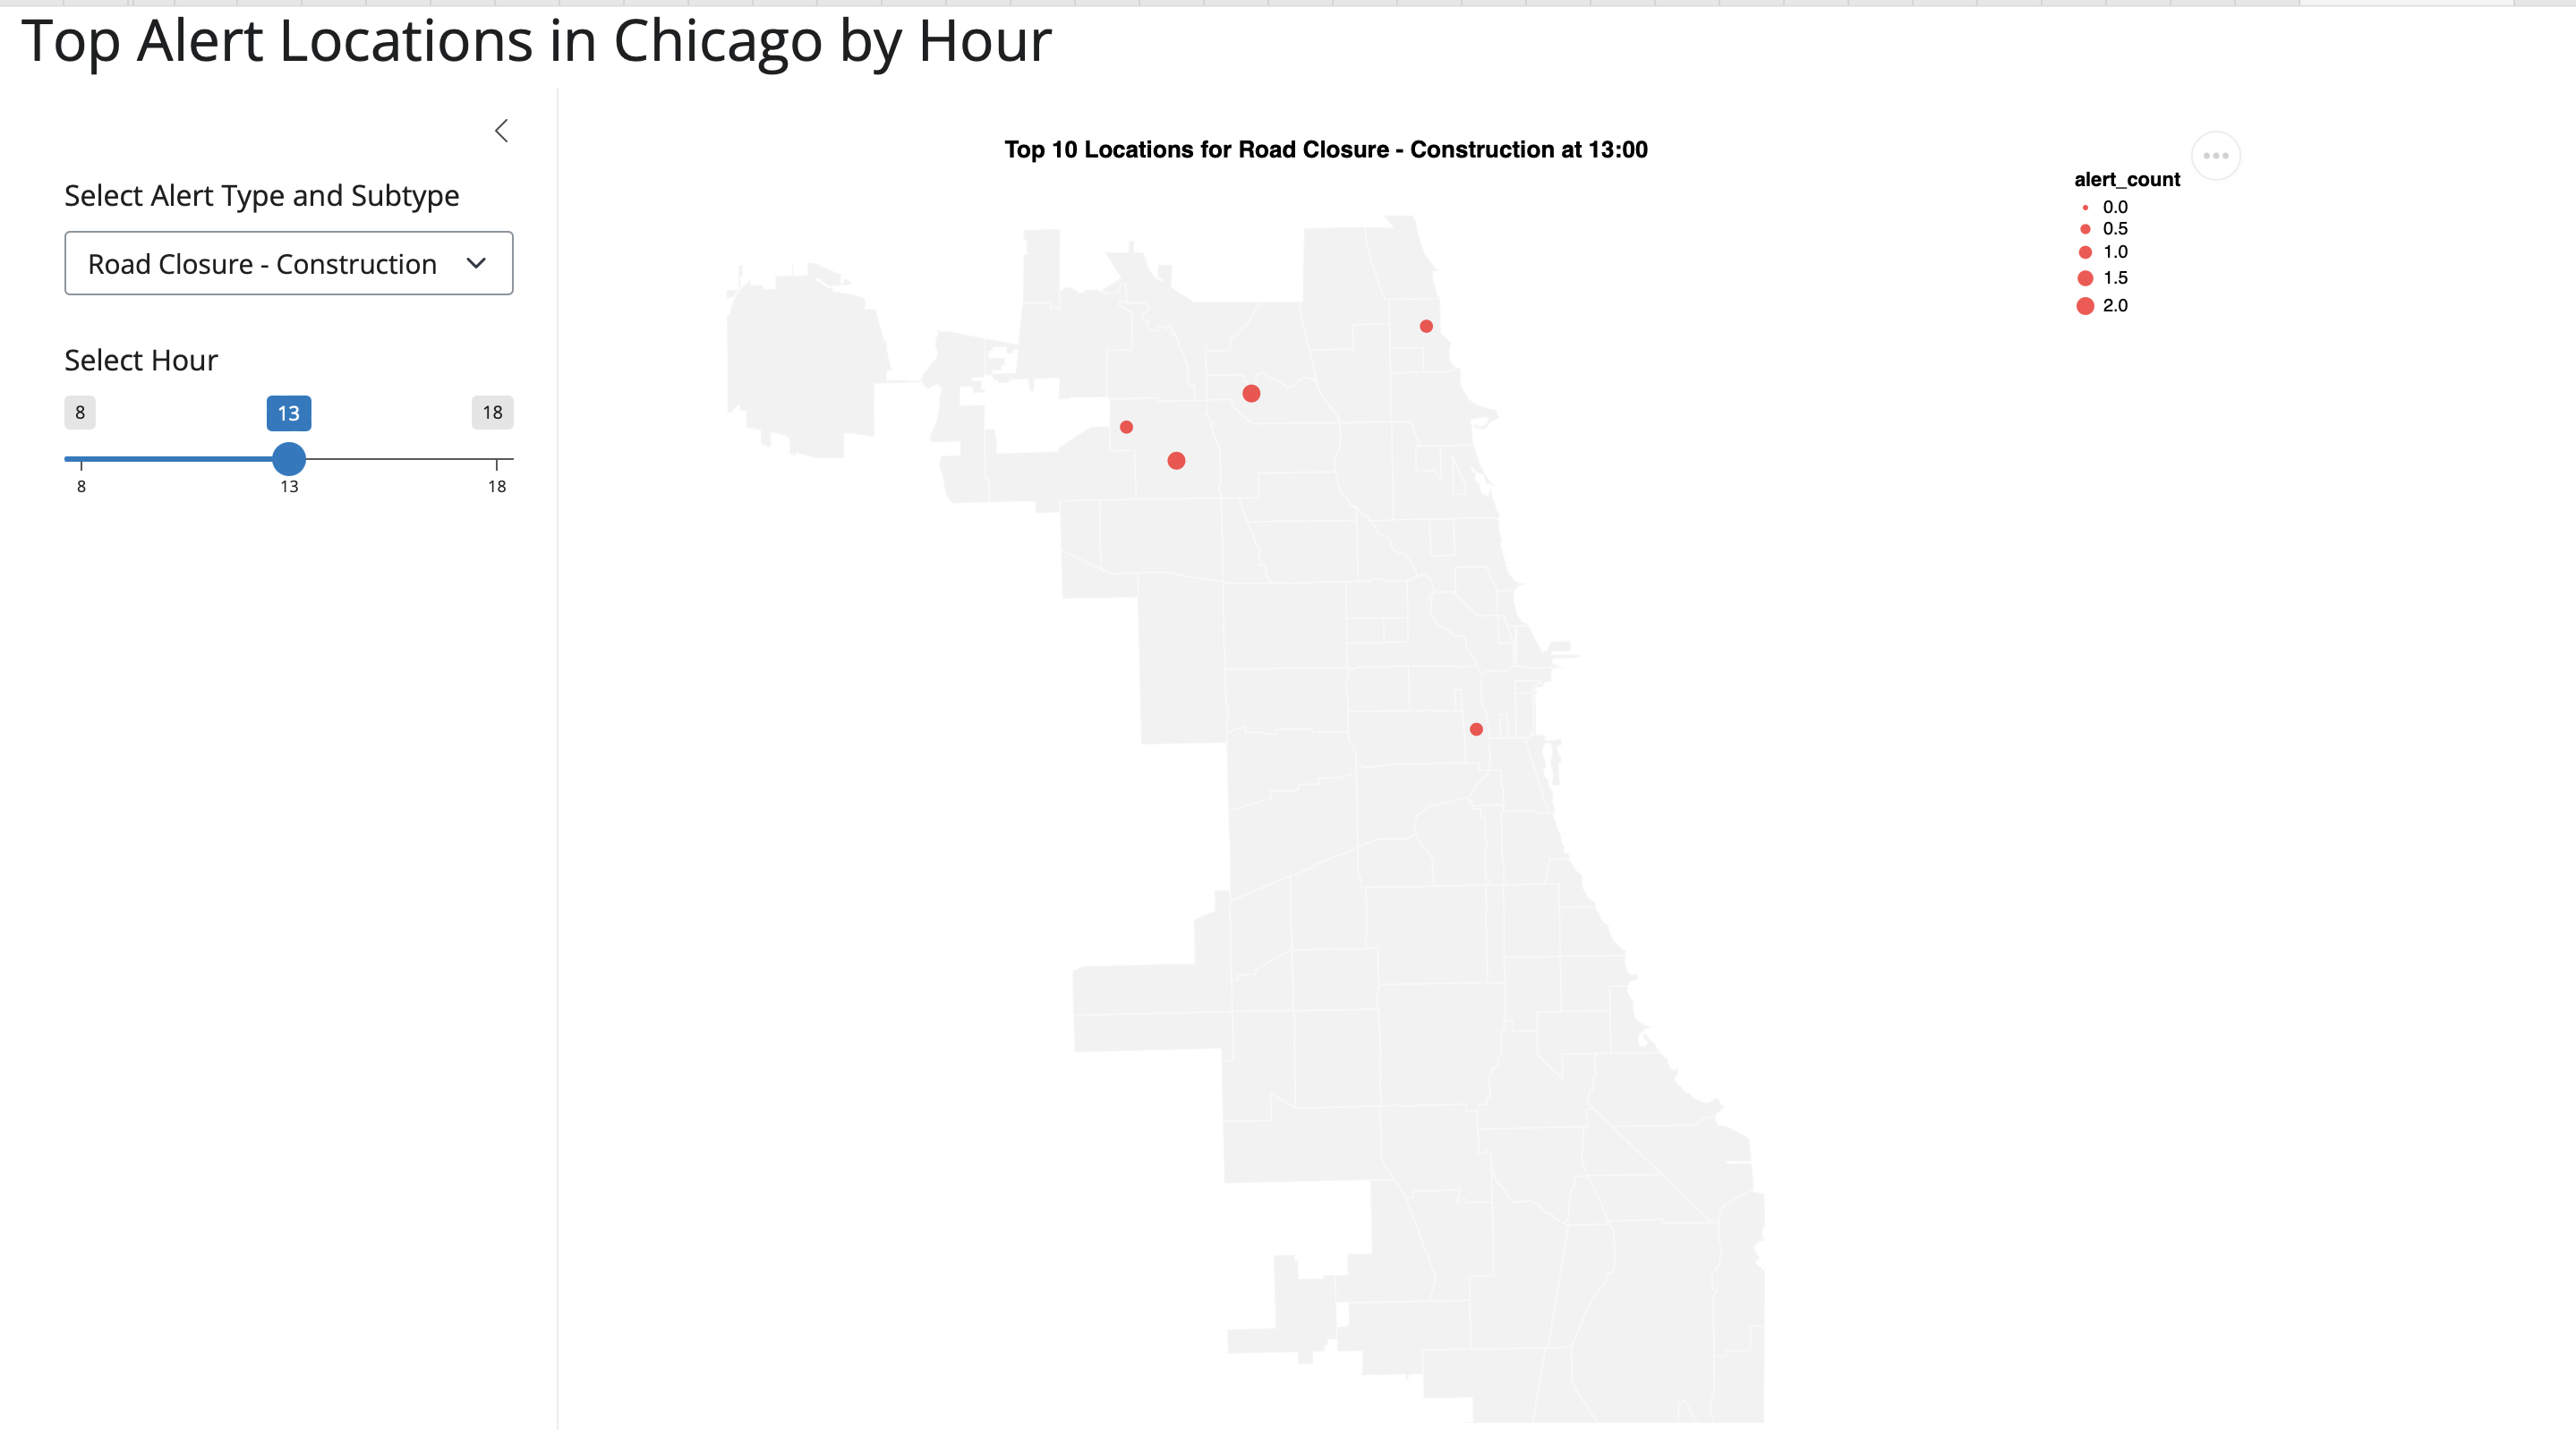
\includegraphics{.ps6/images/6.png}
  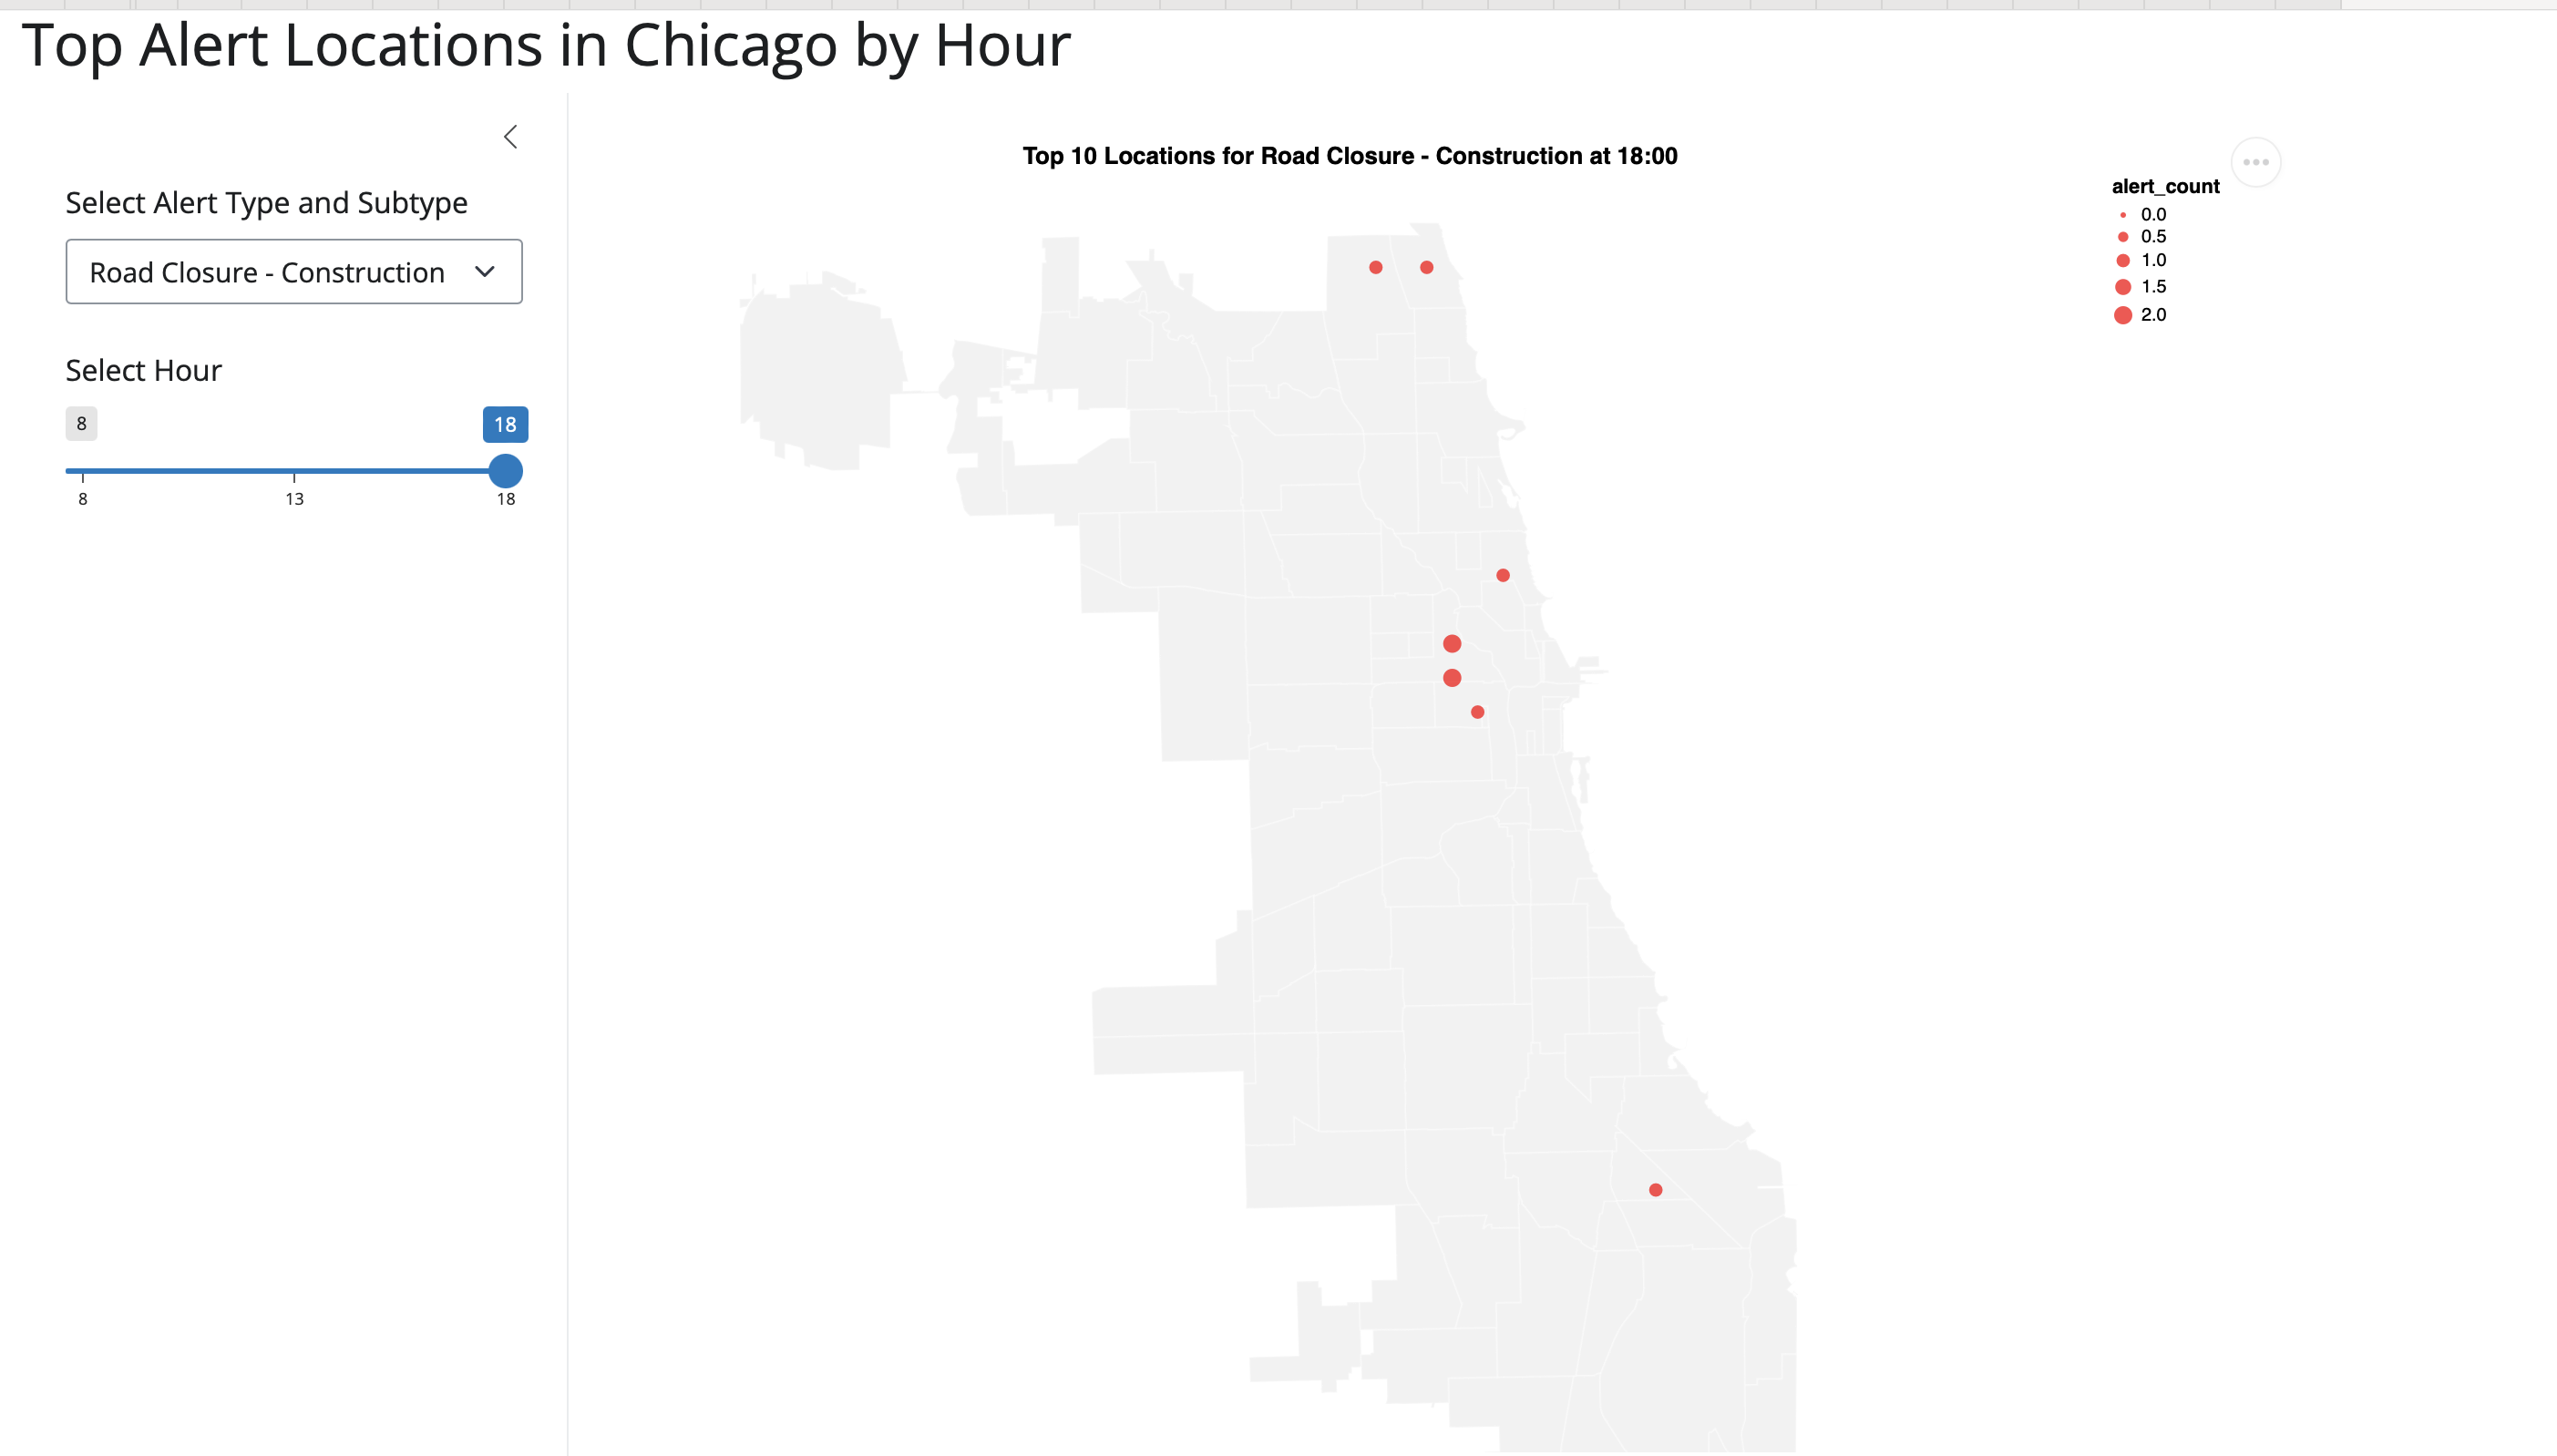
\includegraphics{.ps6/images/7.png}
\end{enumerate}

\section*{App \#3: Top Location by Alert Type and Hour Dashboard (20
points)}\label{app-3-top-location-by-alert-type-and-hour-dashboard-20-points}
\addcontentsline{toc}{section}{App \#3: Top Location by Alert Type and
Hour Dashboard (20 points)}

\begin{enumerate}
\def\labelenumi{\arabic{enumi}.}
\tightlist
\item
\end{enumerate}

\begin{enumerate}
\def\labelenumi{\alph{enumi}.}
\item
  For this app, it might be better to not collapse the dataset by range
  of hours initially. Instead, allow the app to dynamically aggregate
  data based on user-selected hour ranges. This approach provides more
  flexibility and allows users to explore the data in various ways.
\item
\end{enumerate}

\begin{enumerate}
\def\labelenumi{\arabic{enumi}.}
\setcounter{enumi}{1}
\tightlist
\item
\end{enumerate}

\begin{enumerate}
\def\labelenumi{\alph{enumi}.}
\item
  This is the UI before I adjust the size of the circles, which does not
  have the switch button. I put it here for reference.
  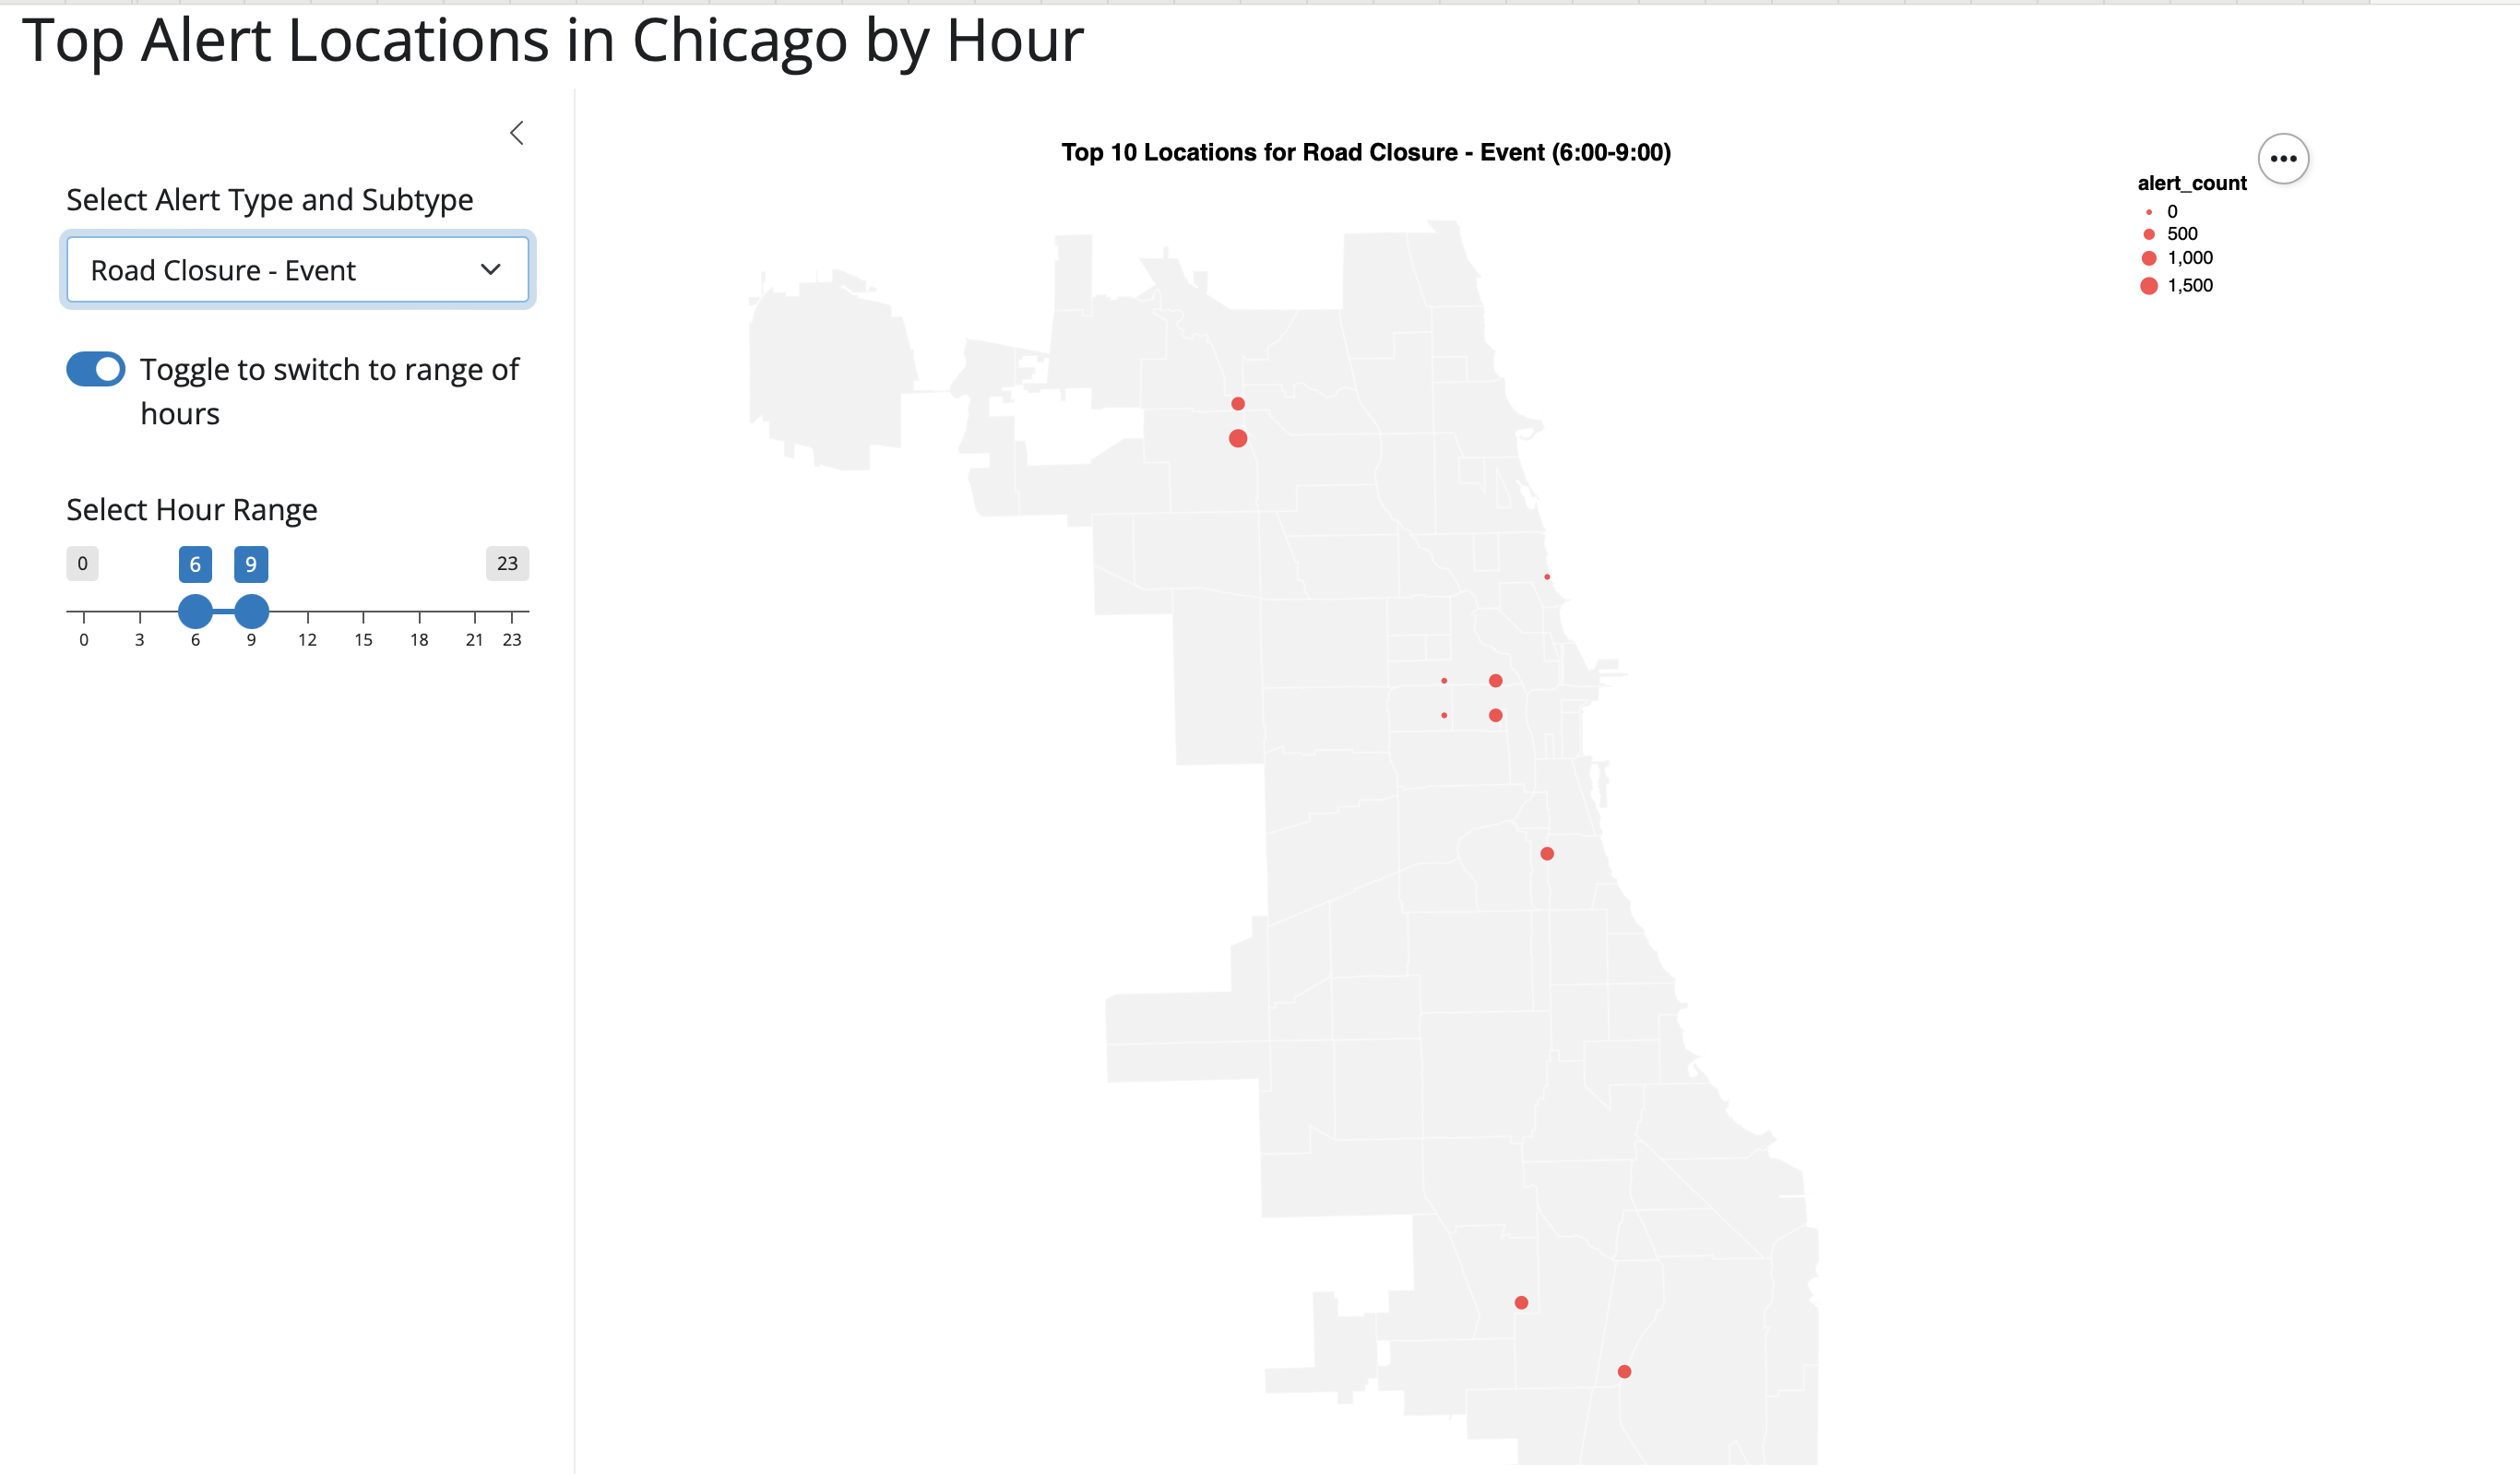
\includegraphics{.ps6/images/11.png} This one is after I adjust the
  size of the circles, which is why it already has the switch button.
\item
  \begin{figure}[H]

  {\centering 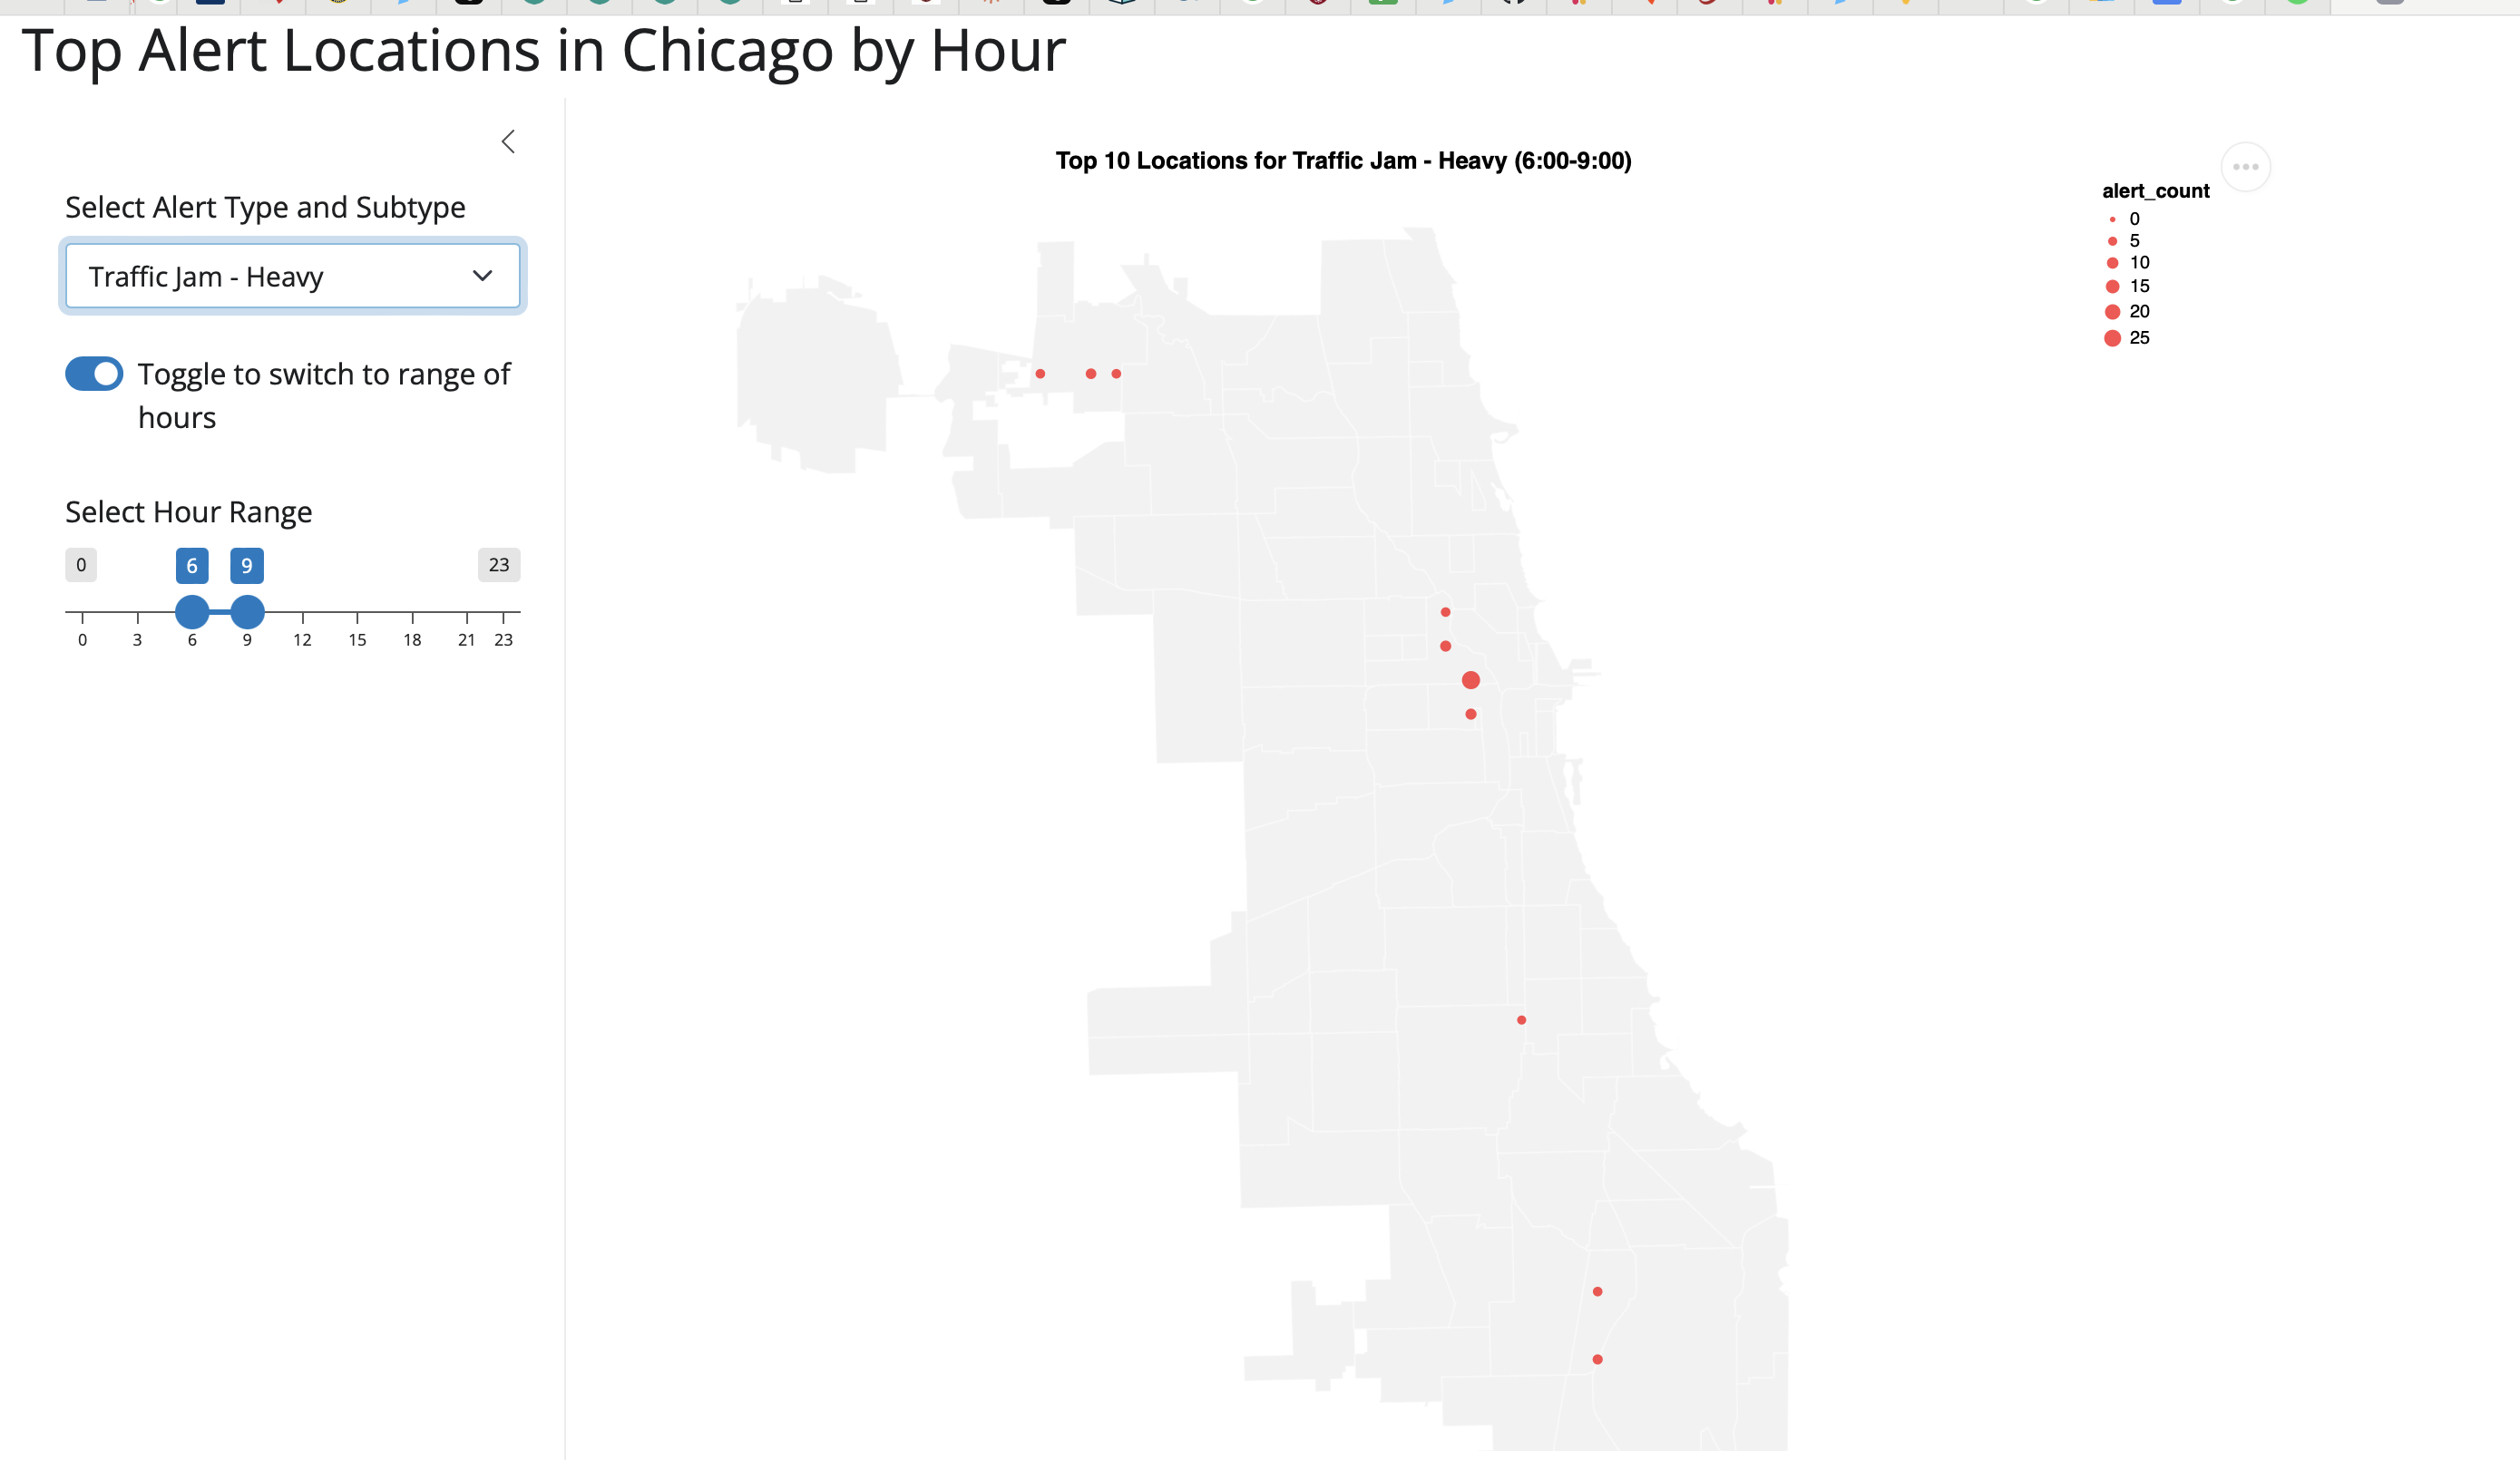
\includegraphics{.ps6/images/12.png}

  }

  \caption{Slider range}

  \end{figure}%
\end{enumerate}

\begin{enumerate}
\def\labelenumi{\arabic{enumi}.}
\setcounter{enumi}{2}
\tightlist
\item
\end{enumerate}

\begin{enumerate}
\def\labelenumi{\alph{enumi}.}
\item
  The possible values are True or 1 when the switch button is on, and
  False or 0 when the switch button is off.
  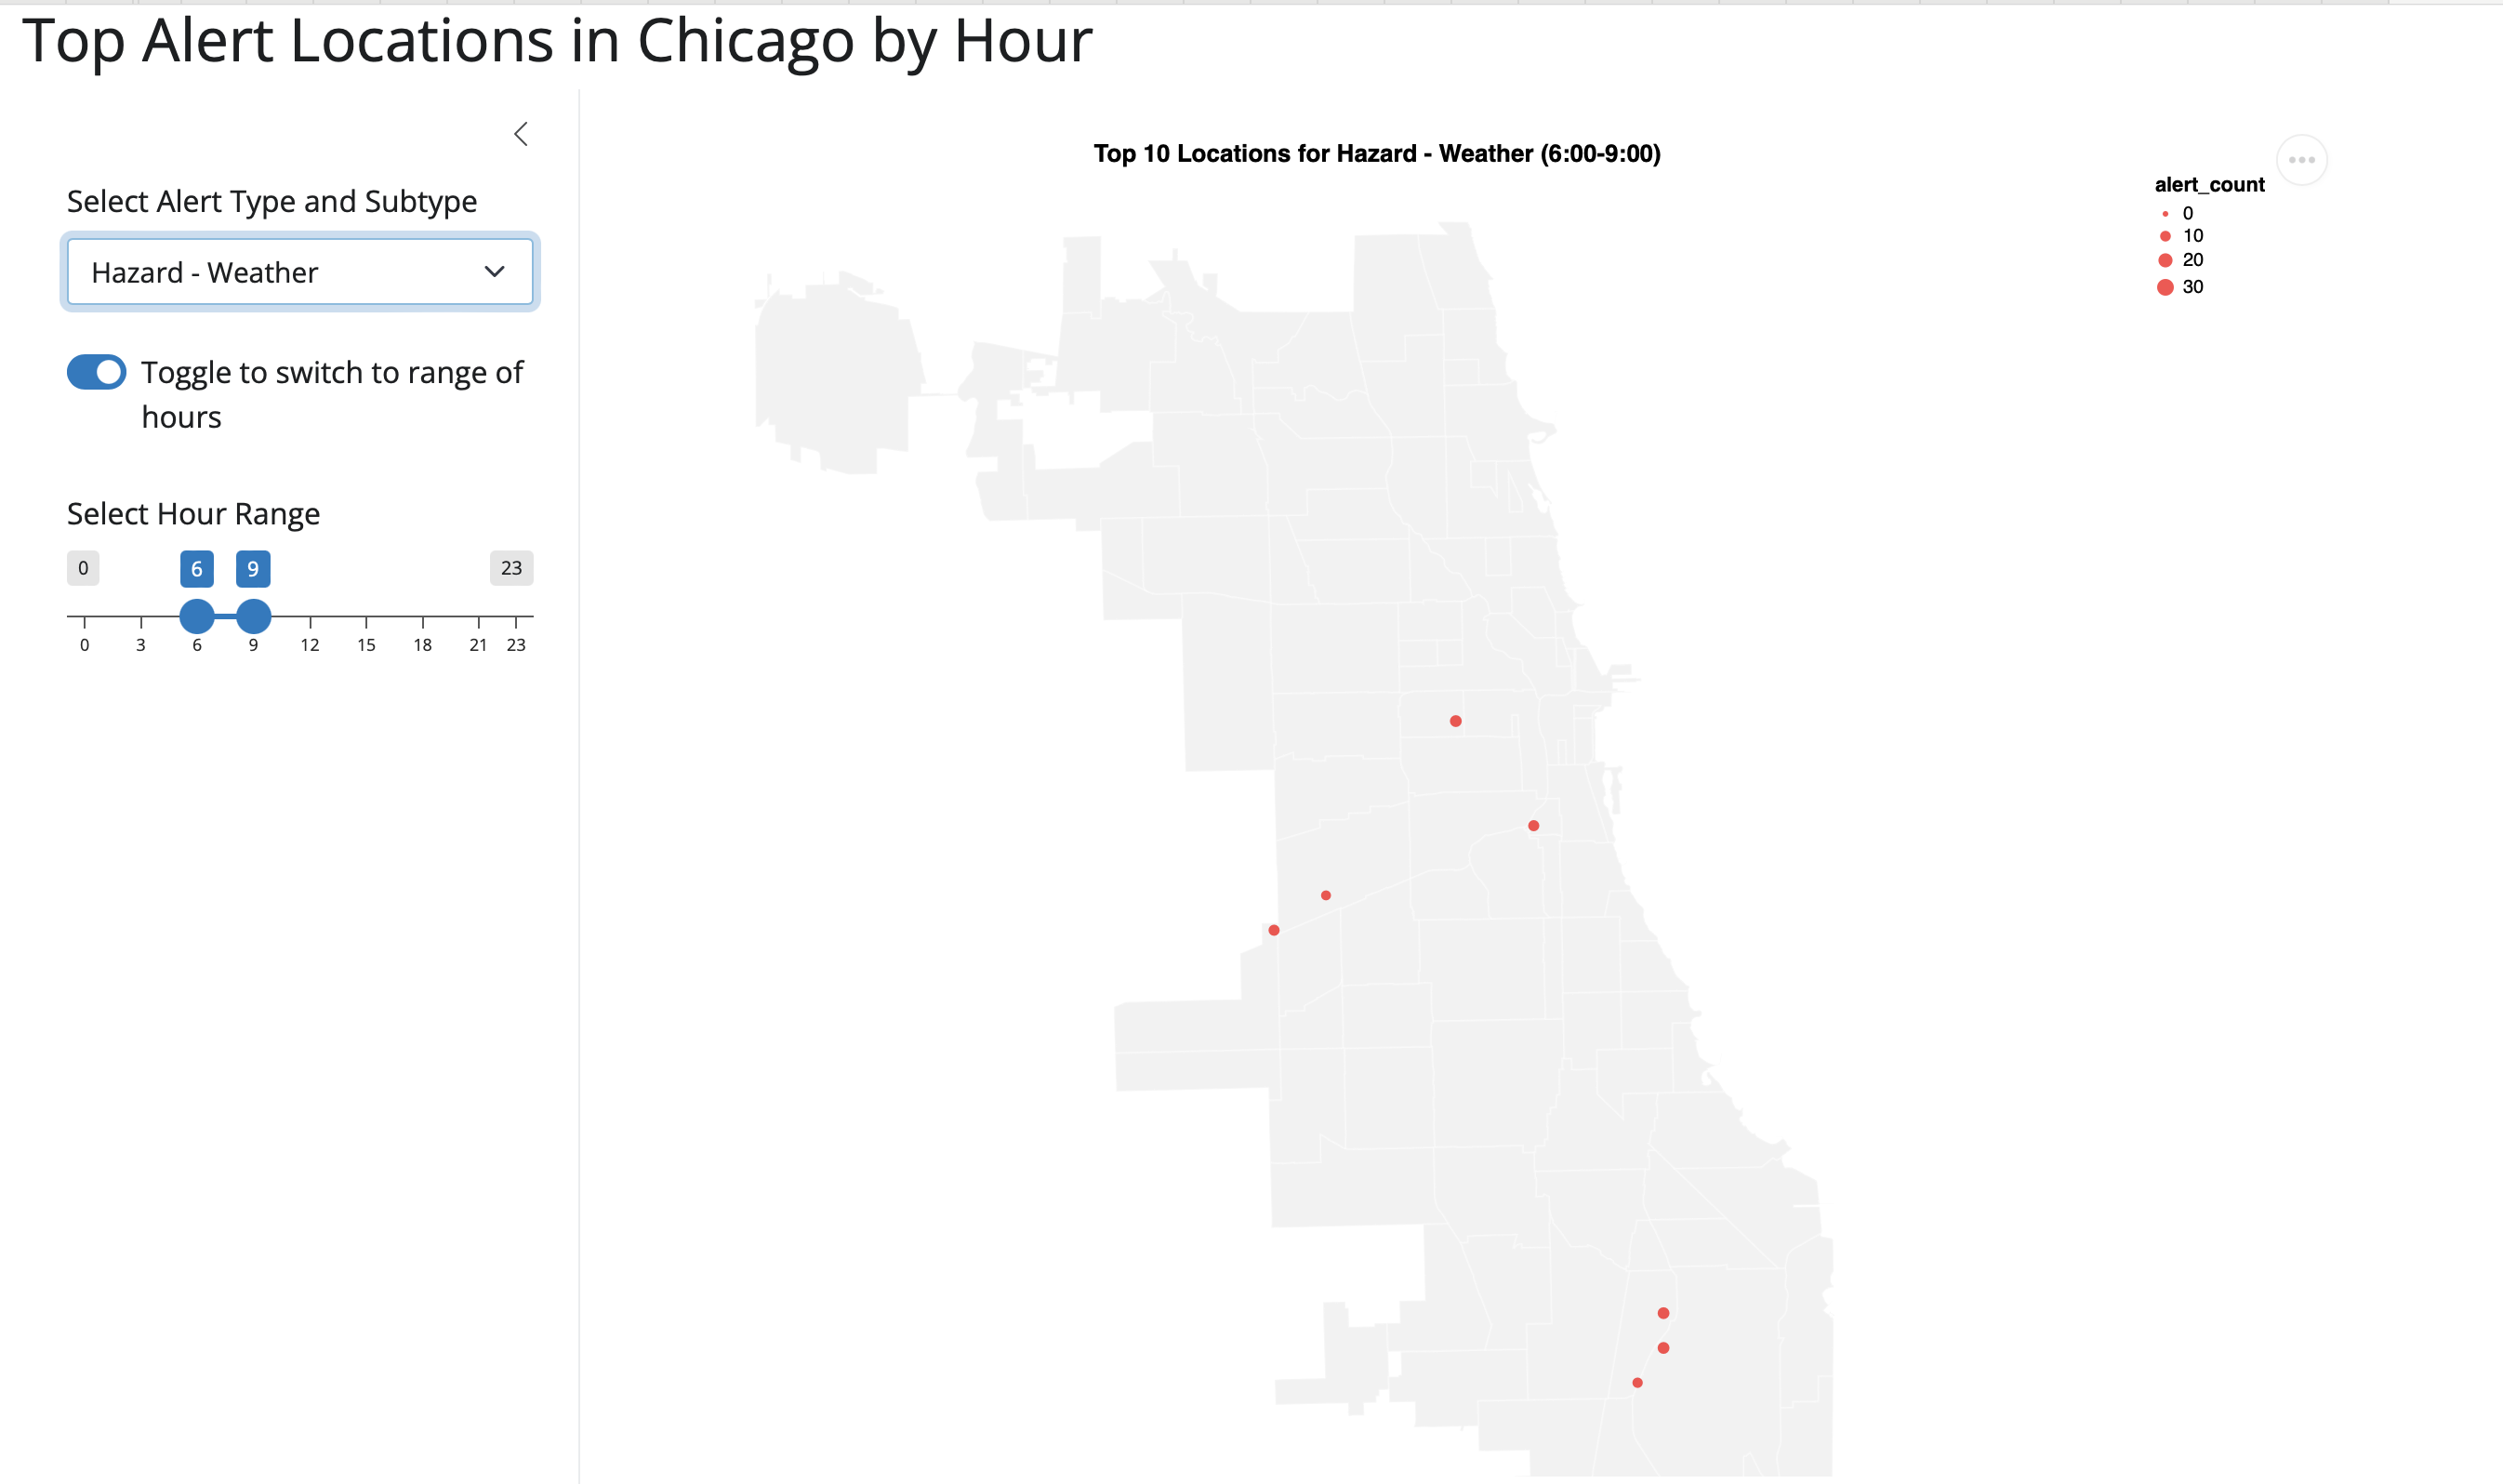
\includegraphics{.ps6/images/13.png}
\item
  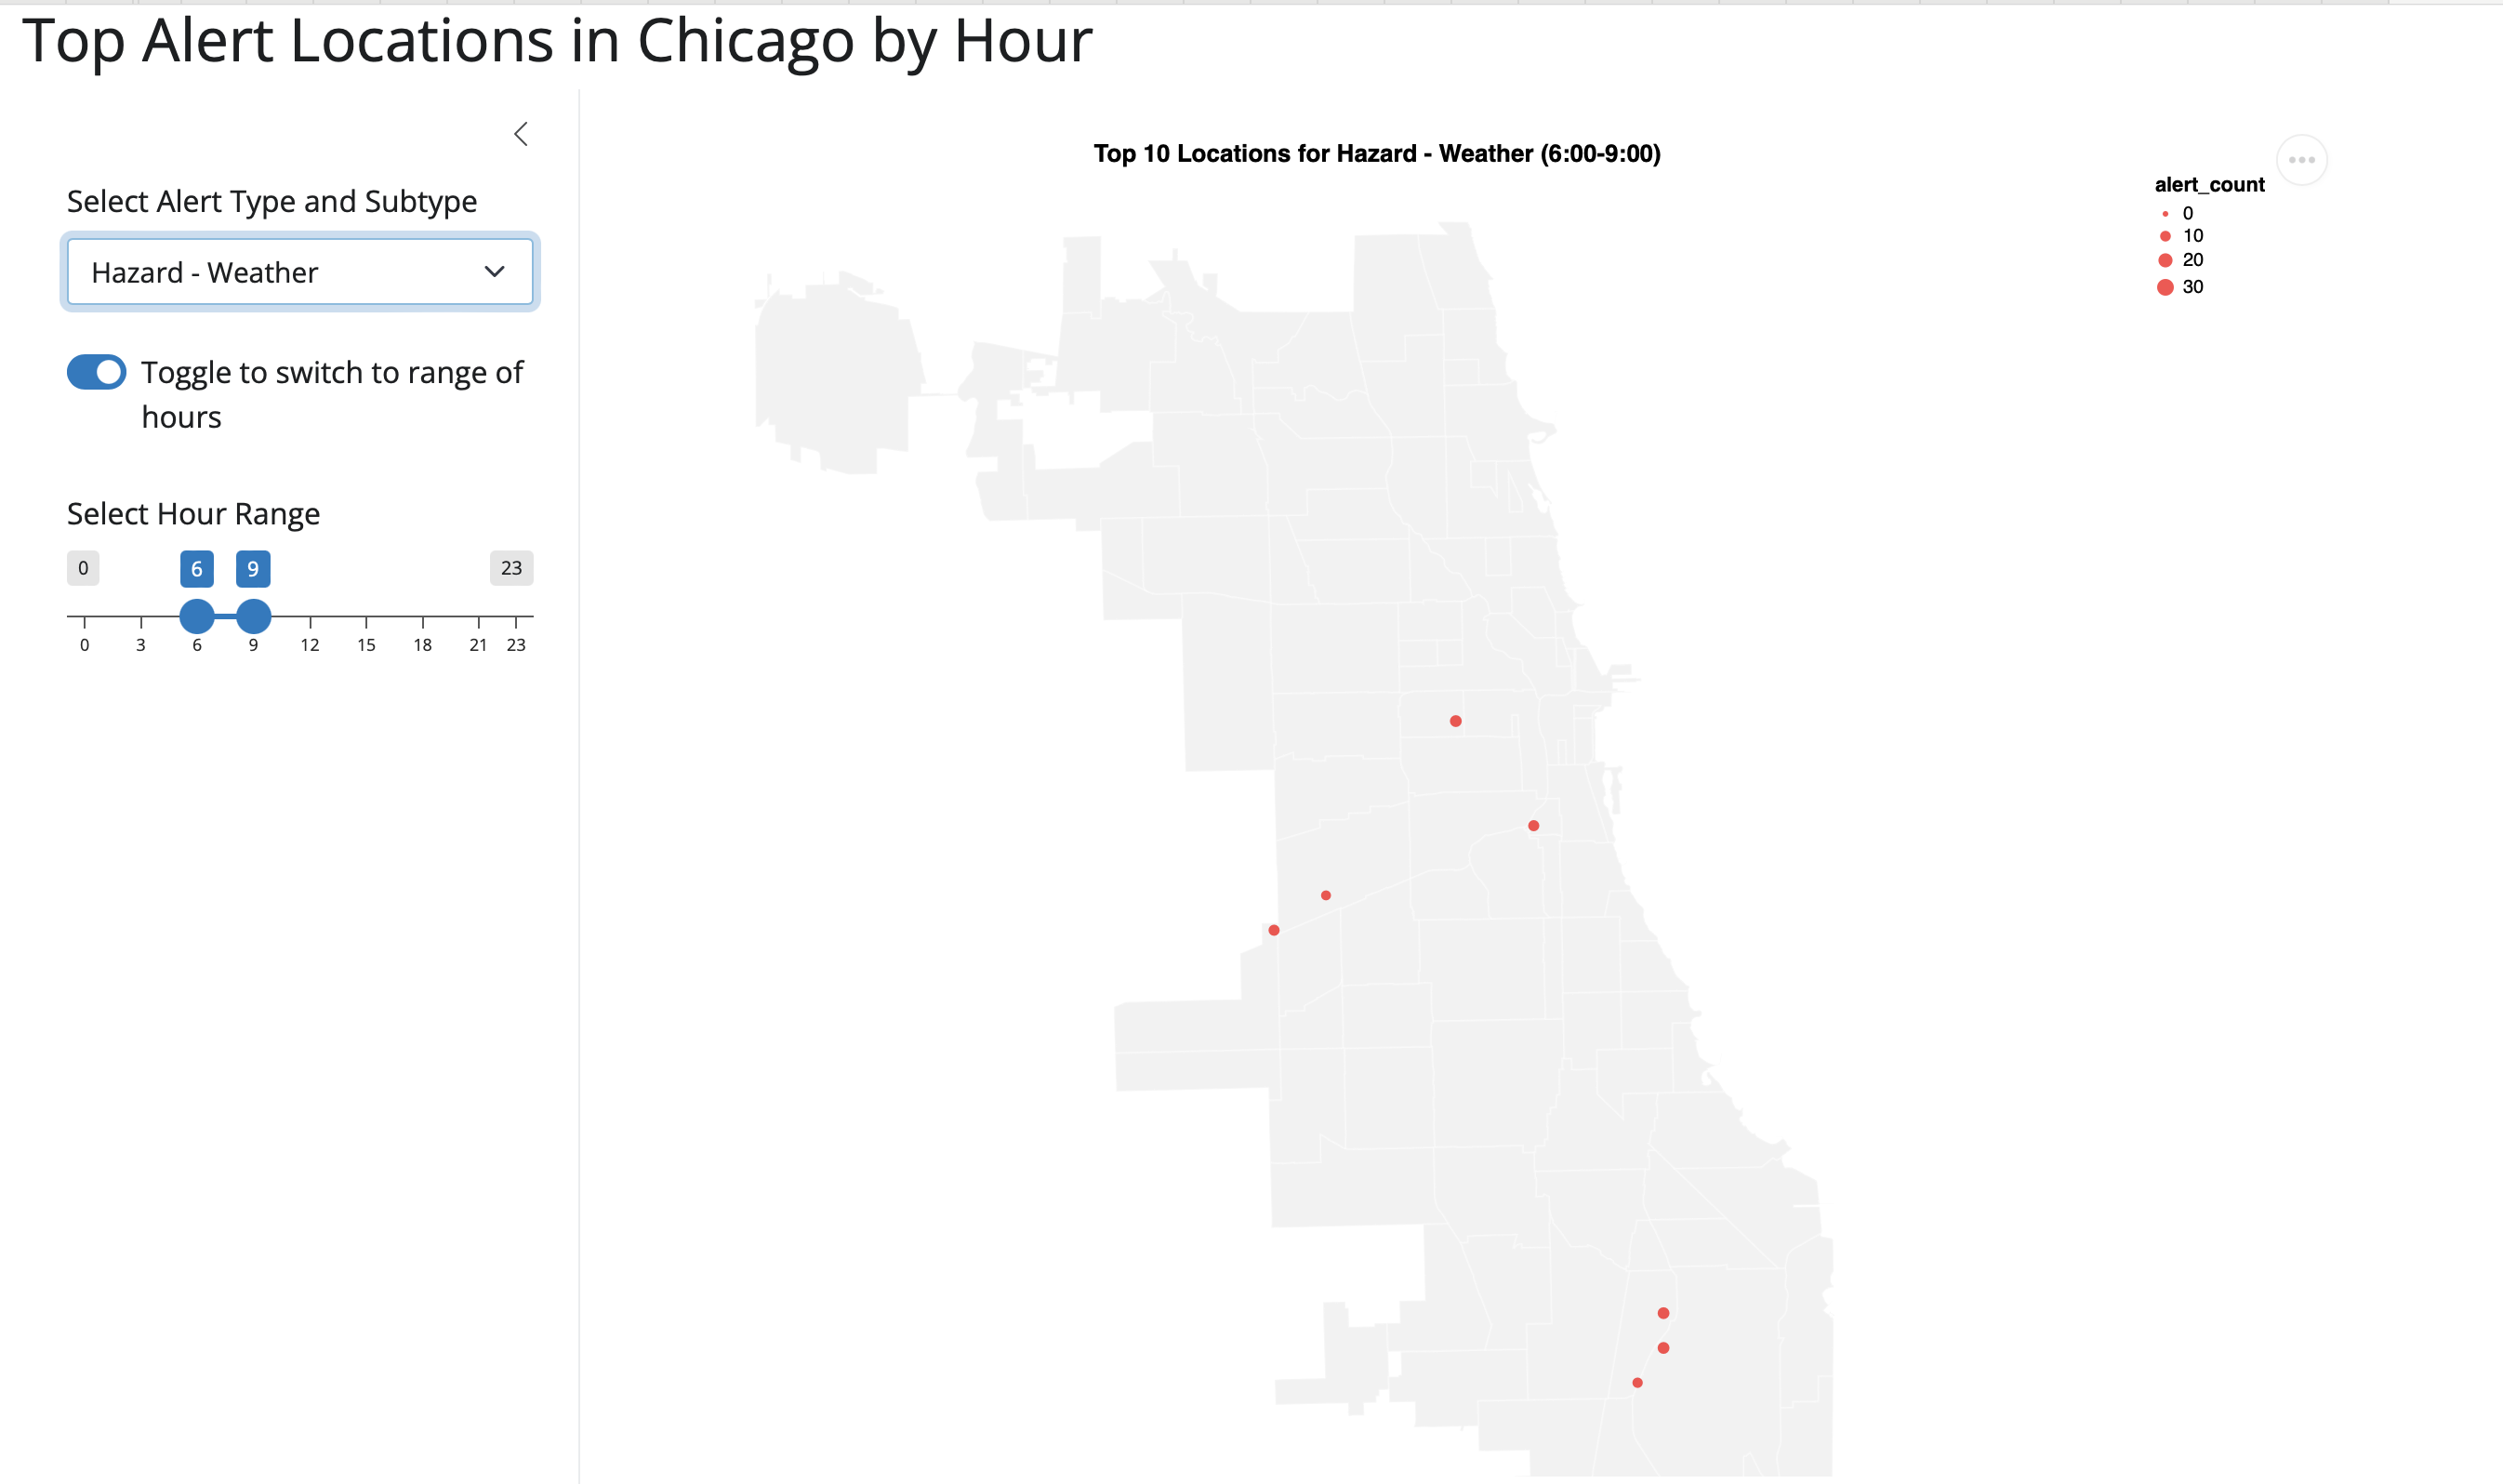
\includegraphics{.ps6/images/13.png}
  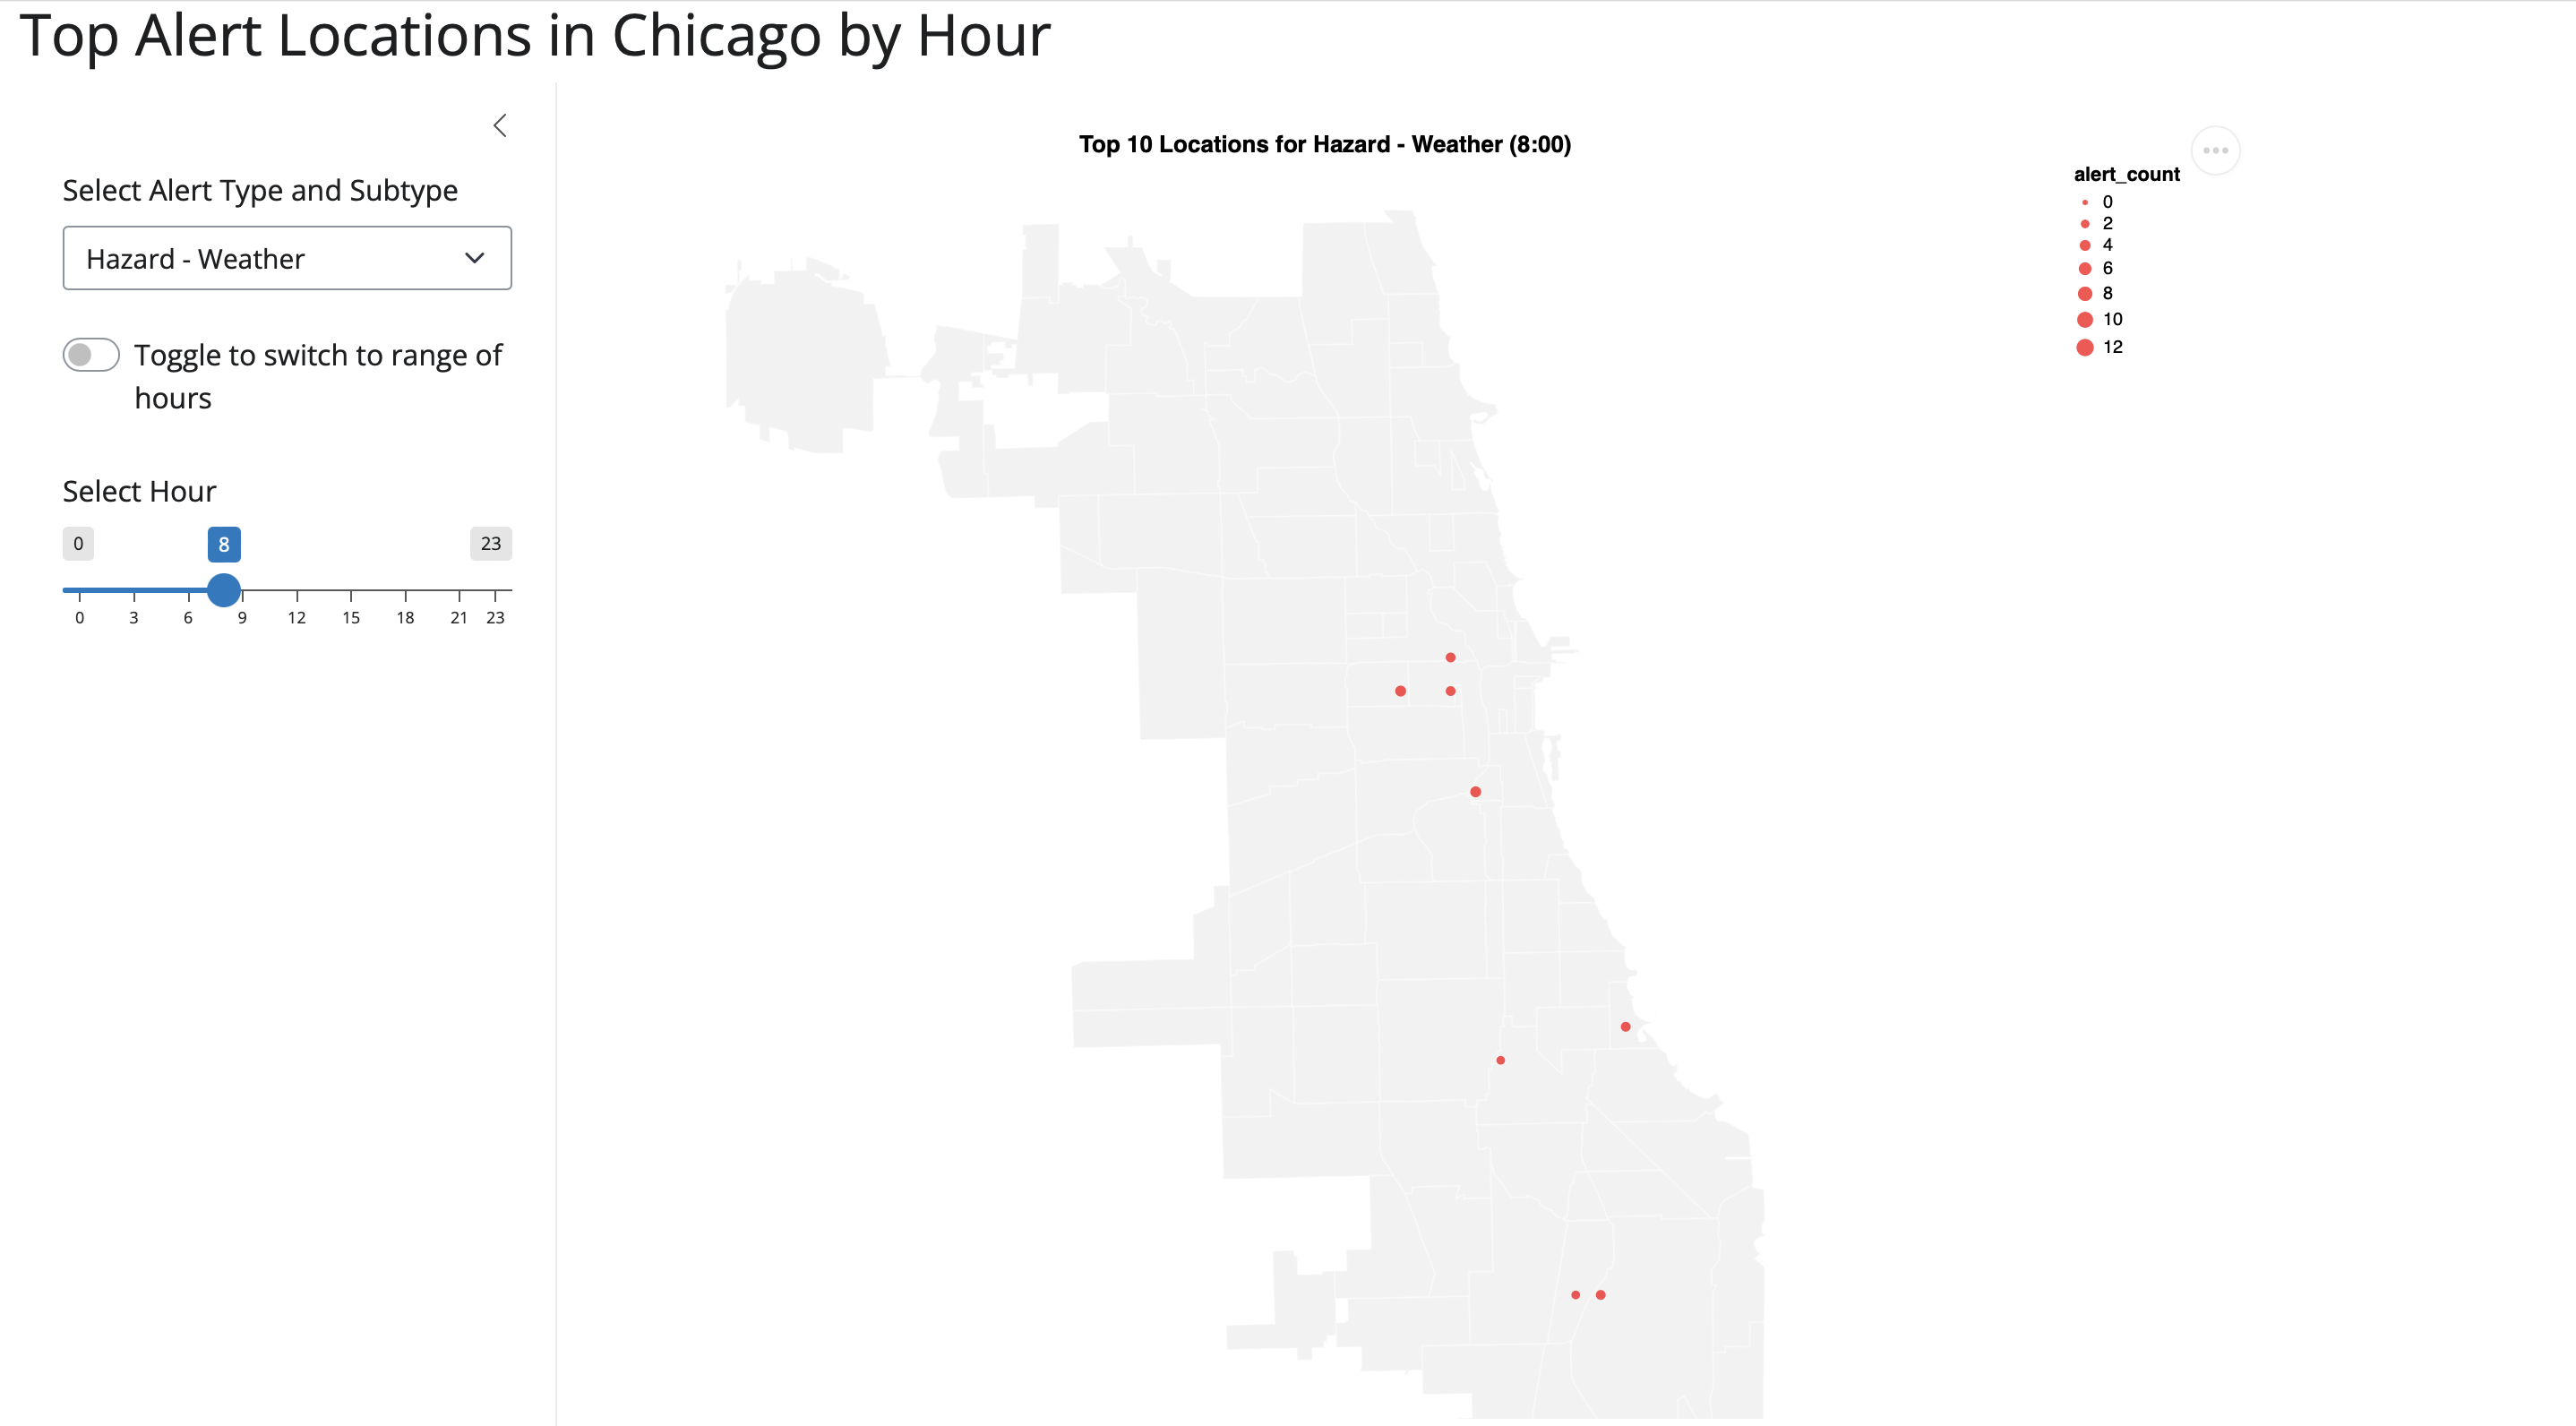
\includegraphics{.ps6/images/14.png}
\item
  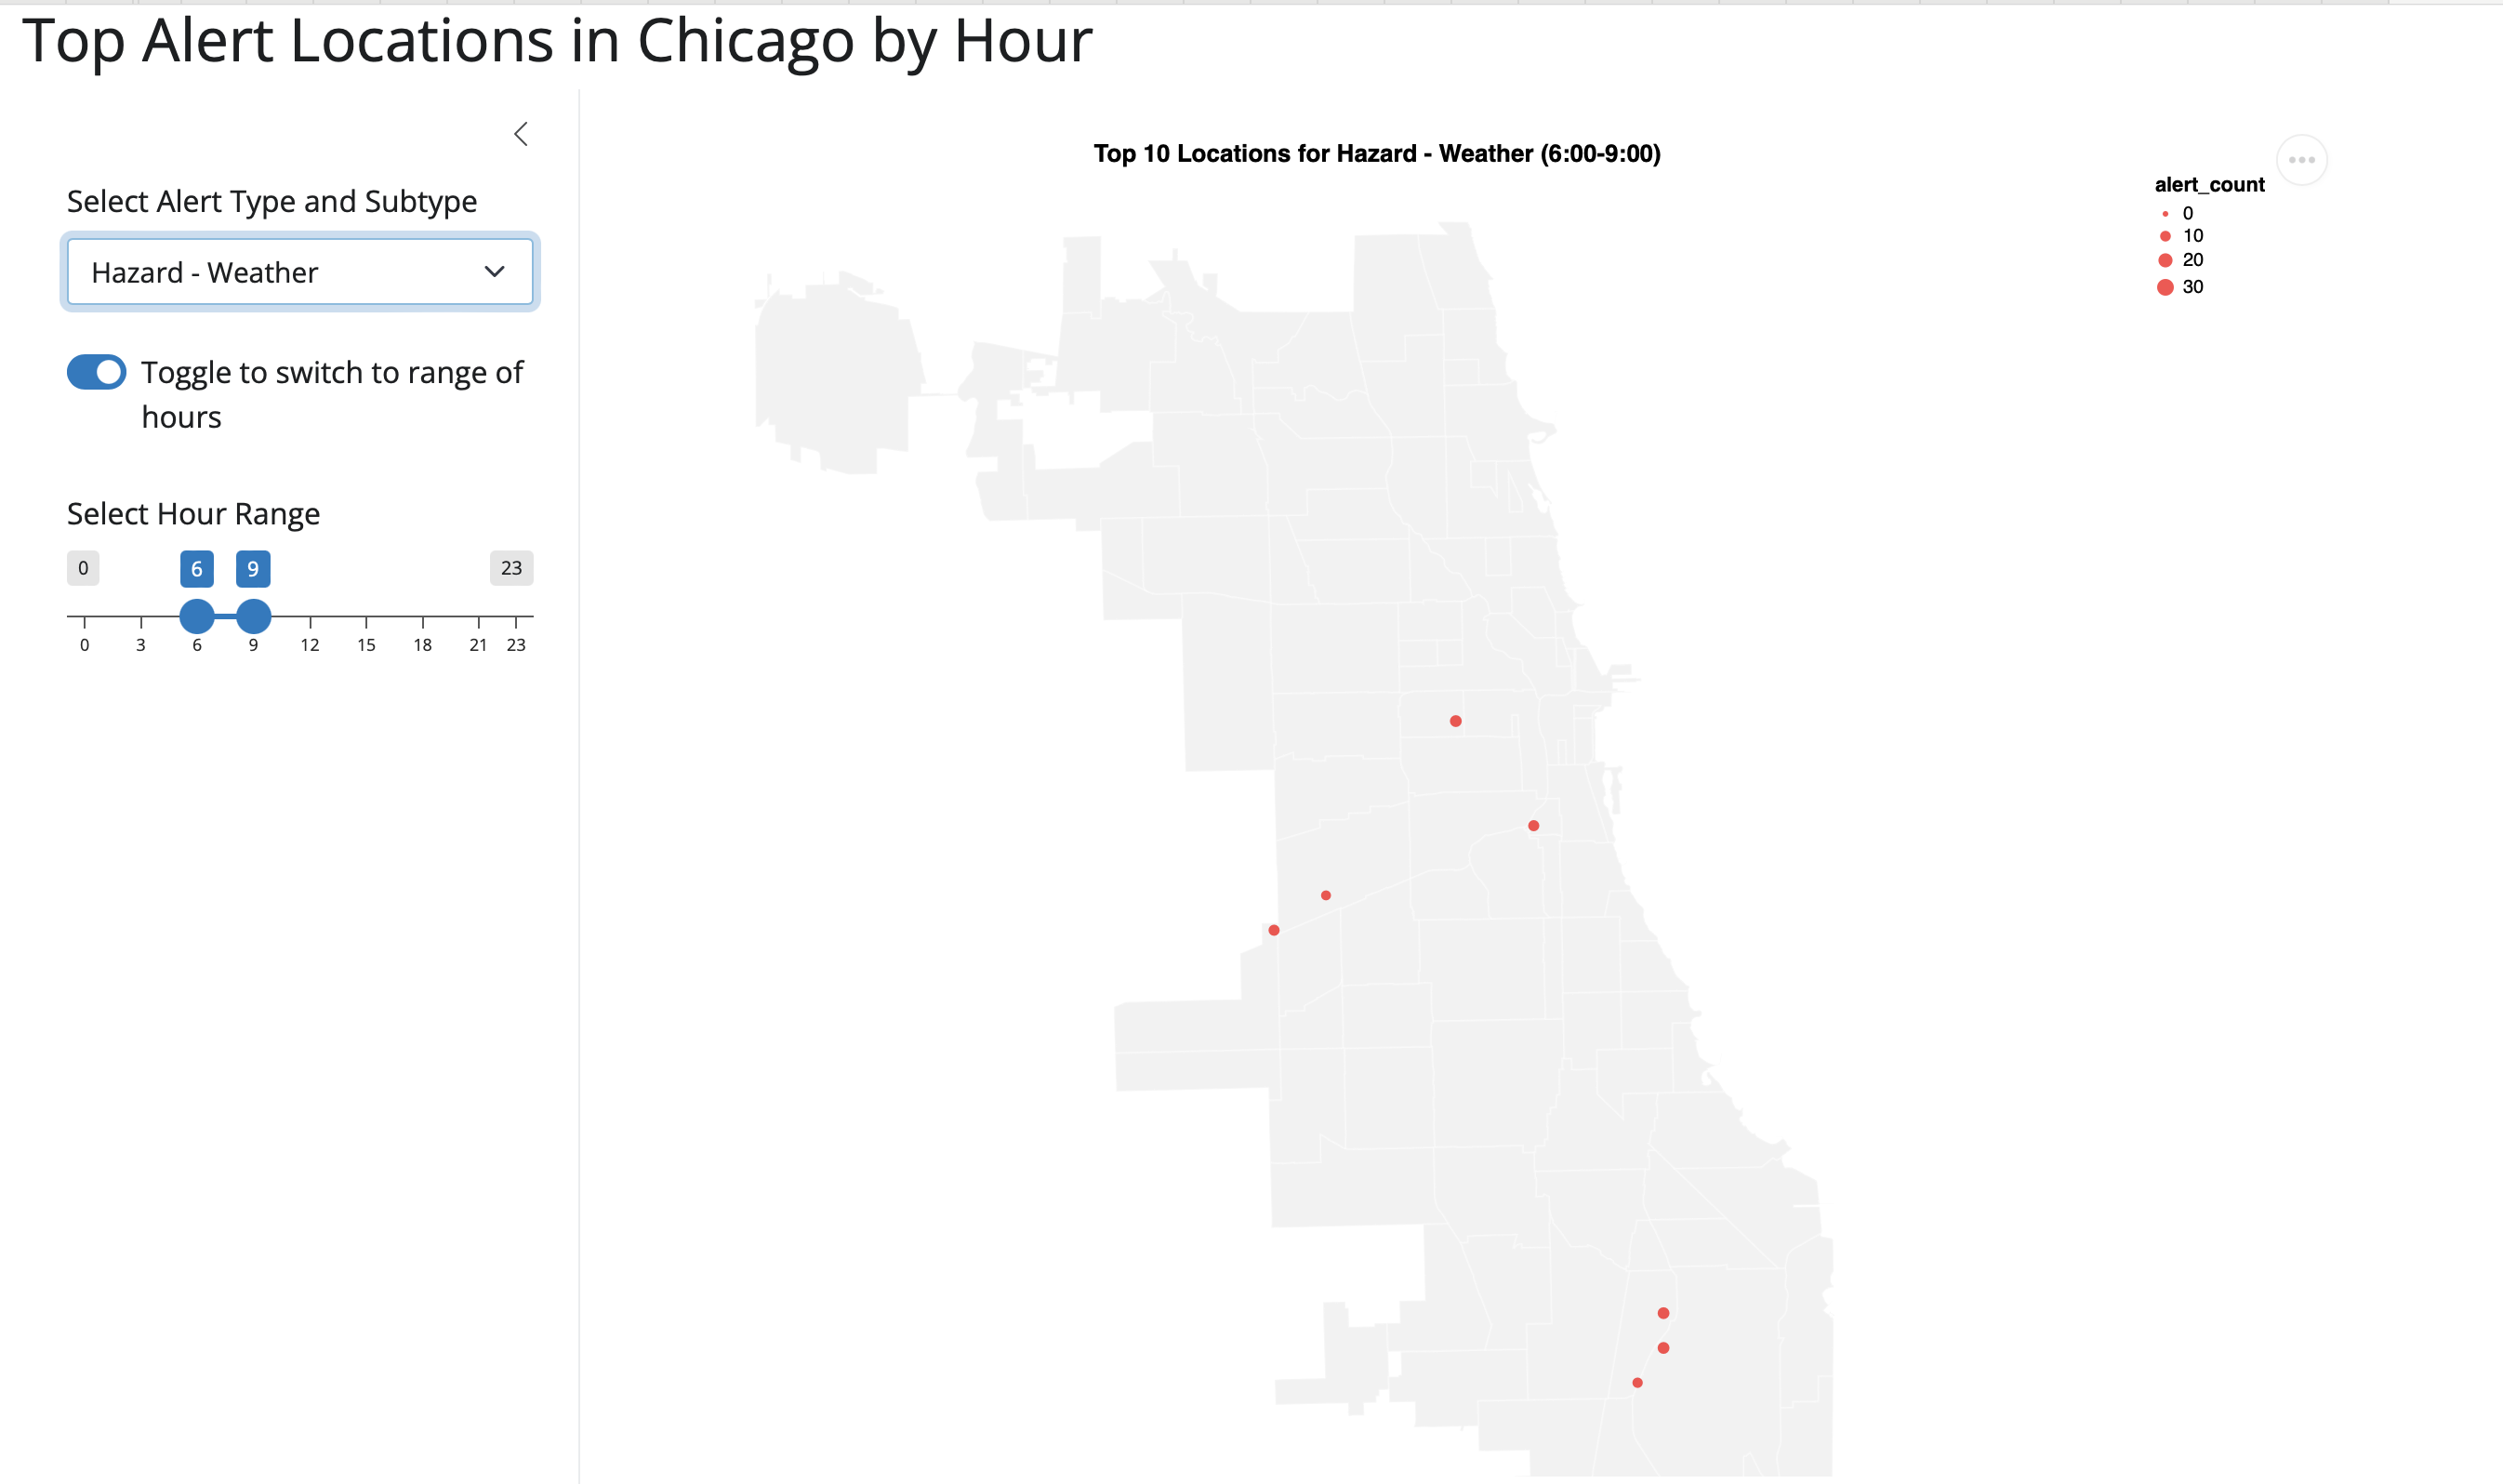
\includegraphics{.ps6/images/13.png}
  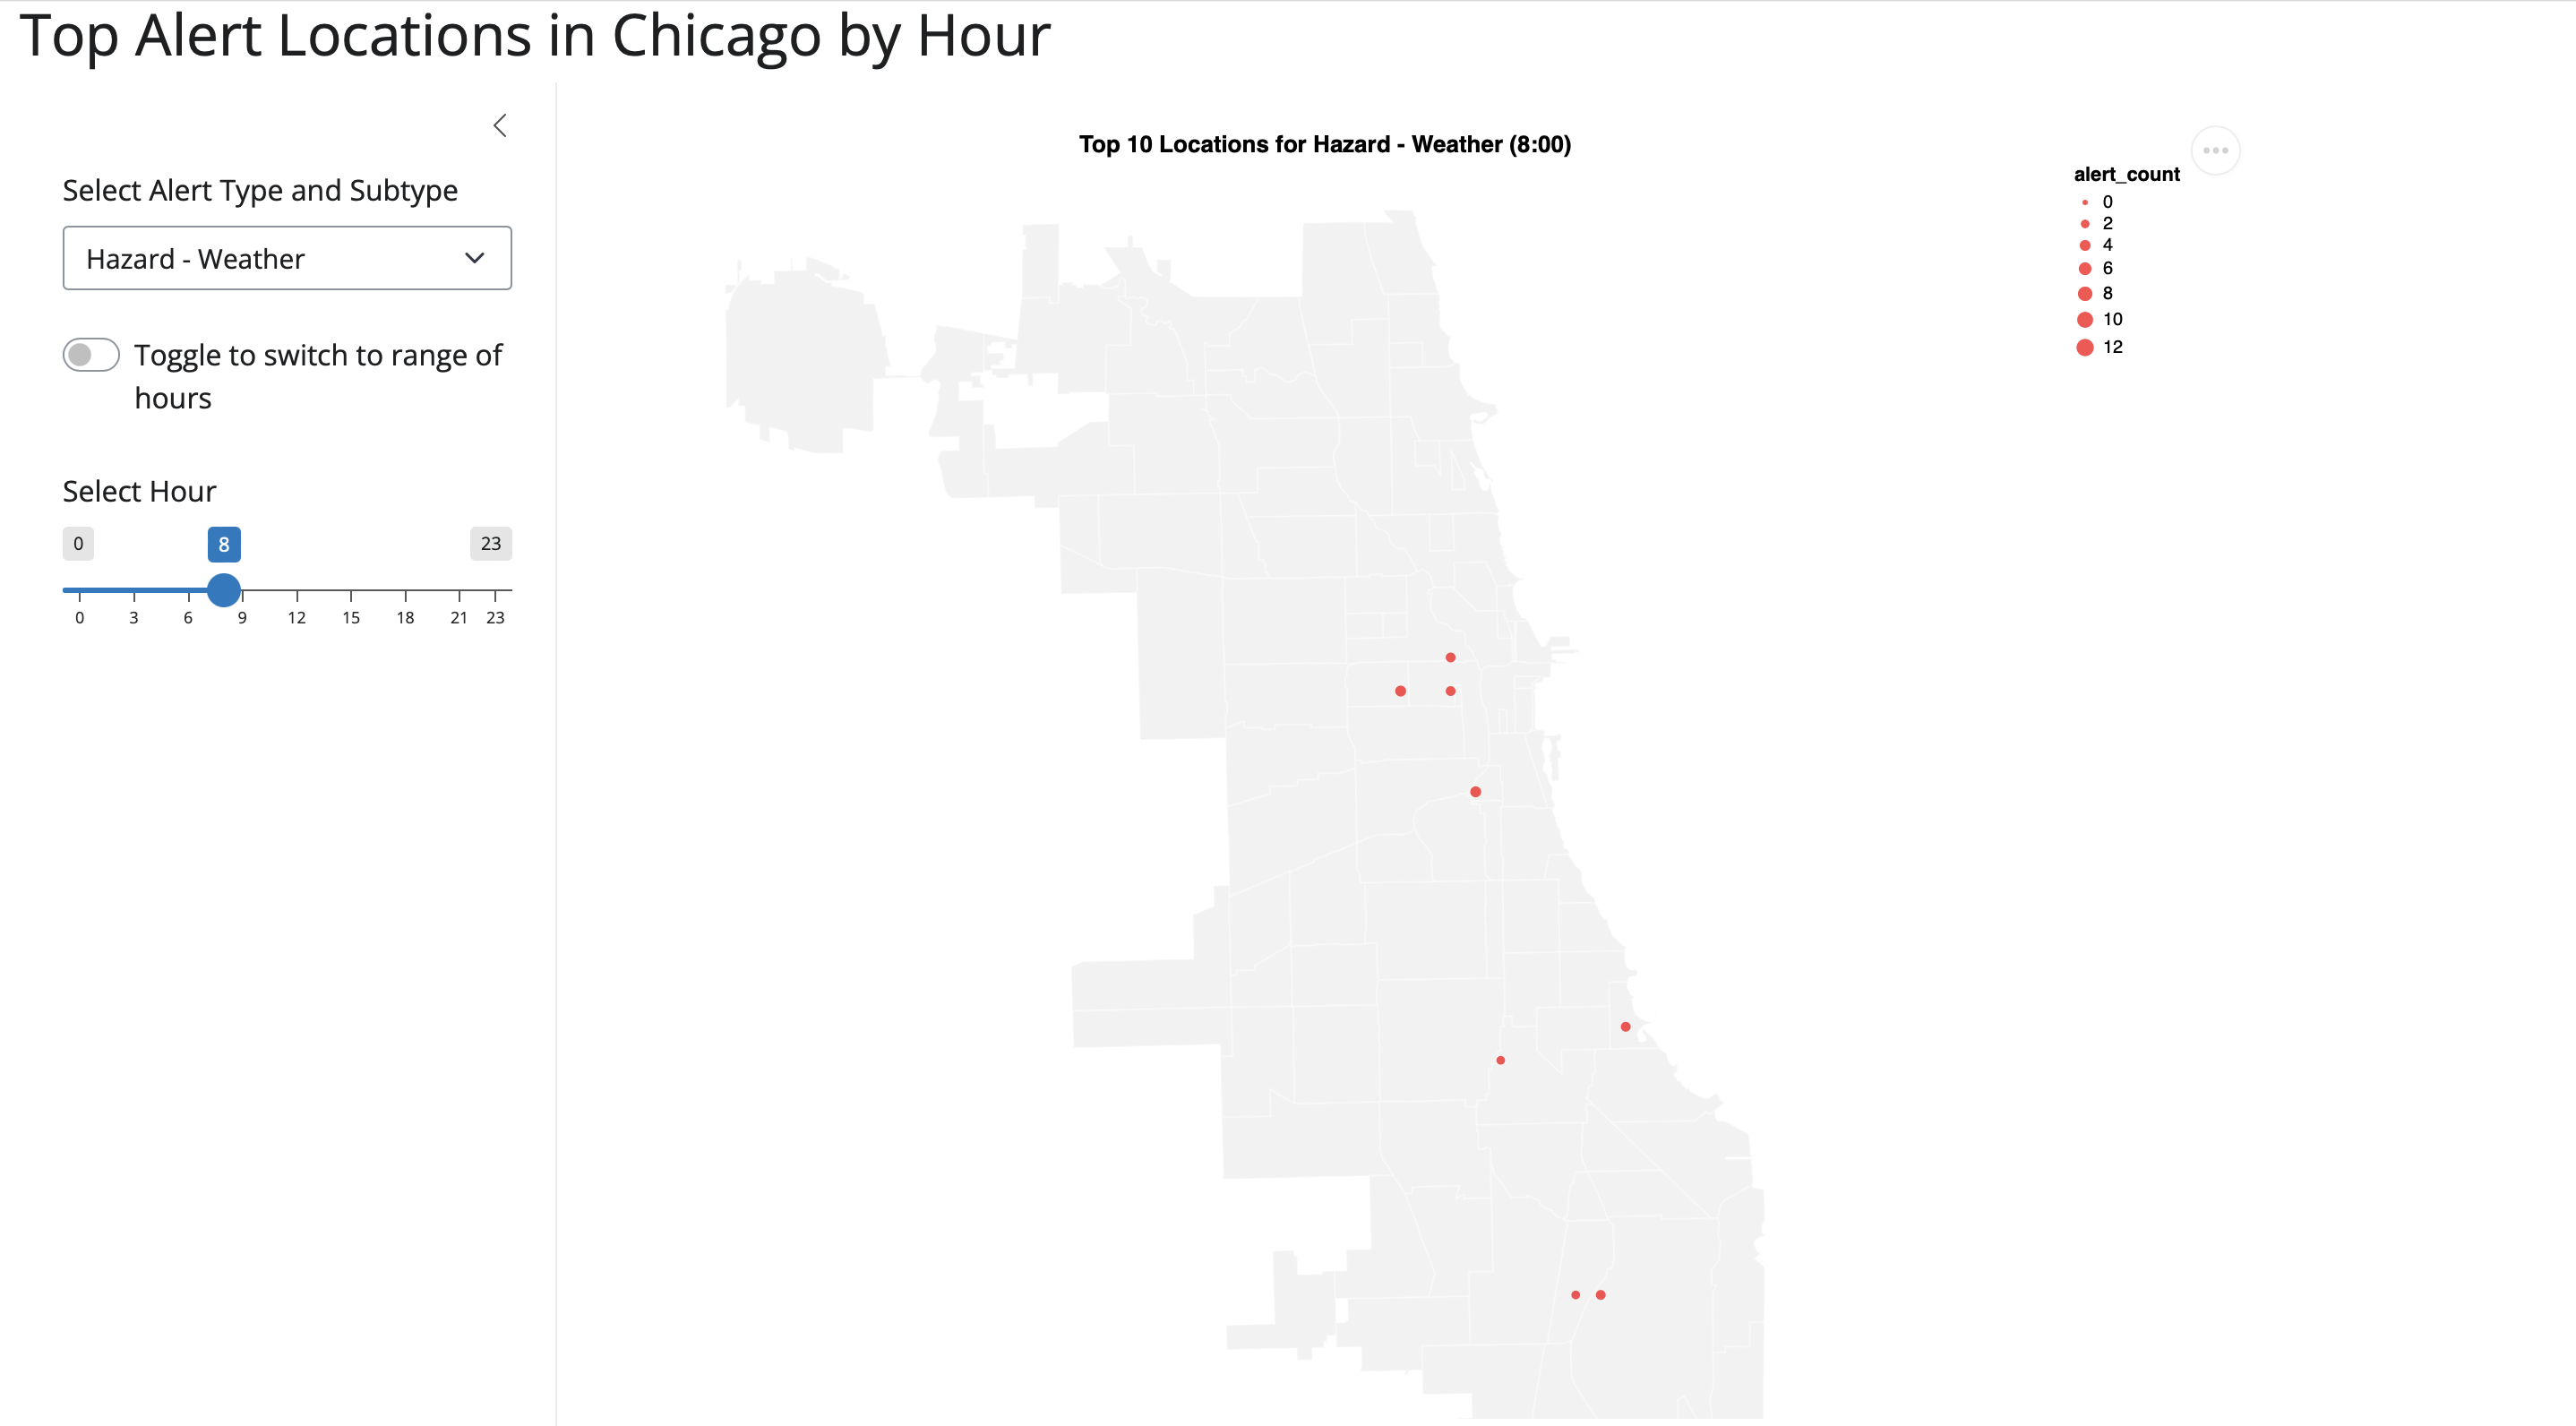
\includegraphics{.ps6/images/14.png}
\item
  I need to add color encoding for time periods into morning and
  afternoon. I need to ensure data is aggredated by the defined time
  periods to reflect the correct number of alerts. I need to add grid
  lines and borders to map, adjist the opacity and fill of the map to
  highlight the points more effectively. I also need to adjust the size
  of the circles to make them better detailedly correspond to the
  longititute and latitude bins.
\end{enumerate}




\end{document}
